\documentclass{TTUPhD}
%%%%%%%%%%%%%%%%%%%%%%%%%%%%%%%%%%%%%%%%%%%%%%%%%%%%%
%%%%% These can be used for revision process %%%%%%%%
%%%%%%%%%%%%%%%%%%%%%%%%%%%%%%%%%%%%%%%%%%%%%%%%%%%%%
%\usepackage{soul} % highlight text with \hl{highlighted text}
%\usepackage{ulem} % strikethrough with \sout{stricken out text}
\usepackage{enumitem}
\usepackage{hyperref}

%\usepackage{setspace} %%% enable the
%\doublespacing        %%% double spacing
%%%%%%%%%%%%%%%%%%%%%%%%%%%%%%%%%%%%%%%%%%%%%%%%%%%%%

%%%%%%%%%%%%%%%%%%%%%%%%%%%%%%%%%%%%%%%%%%%%%%%%%%%%%%%%%%%%%%%%%%%%%%%%%%%%%%%%%%%%%%%%%%%%%%
%%%%%%%%%%%%%%% user-defined variables used in several places of this document %%%%%%%%%%%%%%%
%%%%%%%%%%%%%%%%%%%%%%%%%%%%%%%%%%%%%%%%%%%%%%%%%%%%%%%%%%%%%%%%%%%%%%%%%%%%%%%%%%%%%%%%%%%%%%
% main information
\newcommand{\AuthorName}{André Brandão Daniel Nunel  Pedro Ferreira  Rafael Direito  Rafael Teixeira} % Author's name
\newcommand{\ThesisTitleENG}{\textit{Serious Games} Para Combate De Artrites Nas Mãos} % Title of thesis in English
\newcommand{\ThesisTitleEST}{\textit{Serious Games} Para Combate De Artrites Nas Mãos} % Title of thesis in Estonian
\newcommand{\Year}{201X} % Year of defence
\newcommand{\ThesisNumber}{2018/2019} % Thesis number given by printing office
%%%%%%%%%%%%%%%%%%%%%%%%%%%%%%%%%%%%%%%%%%%%%%%%%%%%%%%%%%%%%%%%%%%%%%%%%%%%%%%%%%%%
%%% insert here the Bibtex names for the articles contained in the work.         %%%
%%% If more than 3, then: a) expand this list;                                   %%%
%%% and b) modify sections 'List of publications' and 'Appendix A: Publications' %%%
\newcommand{\FirstArticle}{ArticleNo1} % work no. 1,     'ArticleNo1' is the BibTeX label,
\newcommand{\SecondArticle}{ArticleNo2} % article no. 2, it's what you'd use in \cite{ArticleNo1}
\newcommand{\ThirdArticle}{ArticleNo3} % article no. 3   (the entry labels in *.bib file)
%\newcommand{\FourthArticle}{ArticleNo4} % article no. 4
%\newcommand{\FifthArticle}{ArticleNo5} % article no. 5
%%%%%%%%%%%%%%%%%%%%%%%%%%%%%%%%%%%%%%%%%%%%%%%%%%%%%%%%%%%%%%%%%%%%%%%%%%%%%%%%%%%%
% list of bibliography resource files
\newcommand{\BibResources}{references} % list here the bibliography resources used in the work
                                          % that means .bib files with absolute or relative paths,
                                          % separated by a comma (no space). Here the file
                                          % './references.bib' is used
%%%%%%%%%%%%%%%%%%%%%%%%%%%%%%%%%%%%%%%%%%%%%%%%%%%%%%%%%%%%%%%%%%%%%%%%%%%%%%%%%%%%%%%%%%%%%%
%%%%%%%%%             end of common variables (used in several places)                 %%%%%%%
%%%%%%%%%%%%%%%%%%%%%%%%%%%%%%%%%%%%%%%%%%%%%%%%%%%%%%%%%%%%%%%%%%%%%%%%%%%%%%%%%%%%%%%%%%%%%%




\begin{document}
\begin{centering}

%First title  page, English. Should require no manual modification
{\LARGE
Universidade de Aveiro \\
Projeto em Informática \\
\ThesisNumber \\
}
\vspace{3.5cm}
{\huge
\bf{
\ThesisTitleENG \\
}
}
\end{centering}

\vspace{3.2cm}

{\fontsize{16}{19.2} \hspace{-0.53cm} André Brandão \hspace{0.5cm} 84916 \\ Daniel Nunes \hspace{0.81cm} 84793 \\
Pedro Ferreira \hspace{0.61cm} 84735 \\ Rafael Direito \hspace{0.71cm} 84921 \\ Rafael Teixeira \hspace{0.59cm} 84746 \\\\
Orientador: Sérgio Matos \\(Professor Auxiliar do Departamento de Eletrónica, Telecomunicações e Informática da Universidade de Aveiro)} \\
\vspace{2.5cm}%{7.9cm} %PRESS\\

\begin{centering}
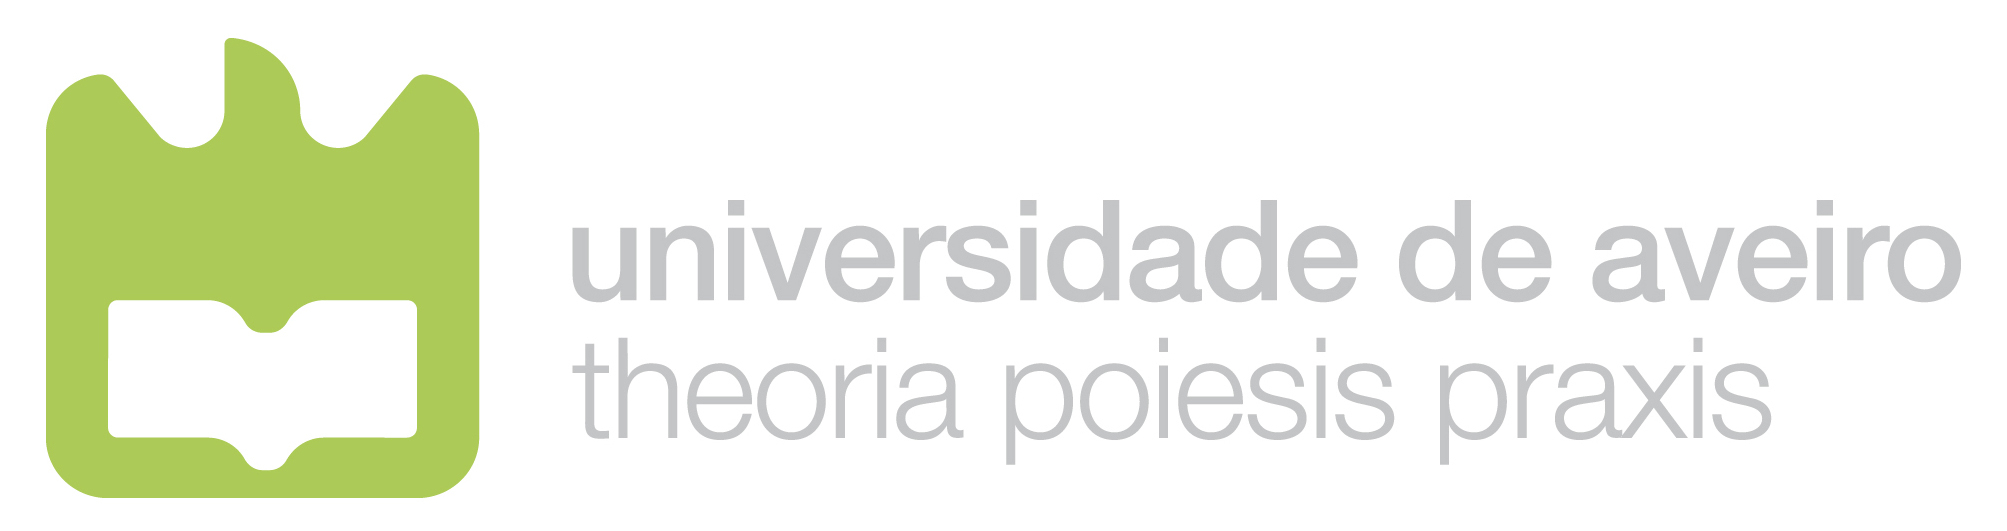
\includegraphics[scale=0.4]{./img/logo_ua.jpg}\\
\end{centering}

\thispagestyle{empty}
%%%%%%%%%%%%%%%%%%%%%%%%%%%%%%%%%
\newpage

\thispagestyle{empty}

% second titlepage, secondary language, should require no manual modification
%\newpage

% its inverse, empty
%\thispagestyle{empty}
%$ \quad $
\newpage


% if table of contents is too long, then use the 'spacing' commands:
%\begin{spacing}{0.1}
\tableofcontents
%\end{spacing}

%\section*{Approbation}
%I presented the results of the thesis at the following conferences:
%\begin{widenumi}
%  \item \textbf{F. Surname}, S. Other, and S. Else. `Title of presentation', Conference name: 8--12 September 2014, Tallinn
%  \item \textbf{F. Surname}, S. Other, and S. Else. `Another title', Some conference, 6--10 October 2014, Prague, Czech Republic
%\end{widenumi}
%
%\newpage

\section*{Palavras-chave}
\addcontentsline{toc}{section}{Palavras-chave}  % adds unnumbered section to the table of contents

\begin{itemize}
    \item Gesture Recognition.
    \item Machine Learning.
    \item Serious Games.
    \item Leap Motion.
    \item Arthritis Treatment.
    \item Treatment monitorization.
\end{itemize}

\section*{Resumo}
\addcontentsline{toc}{section}{Resumo}  % adds unnumbered section to the table of contents

O Arcade Battle é um sistema para ajuda na reabilitação de pacientes com artrite nas mãos.
Através do uso de jogos, os pacientes podem agora fazer os exercícios propostos pelo médico/terapeuta sendo que estes serão os comandos dos jogos arcade.

Para a implementação deste sistema, adotámos uma arquitetura modular onde, por exemplo, qualquer jogo está pronto para receber comandos genéricos, não dependendo assim da forma como estes são obtidos.

Utilizámos árvores de decisão para reconhecimento de gestos, sendo que processo de treino demora menos de 1 minuto, todos os jogos foram desenvolvidos por nós assim como toda a plataforma do paciente e a de gestão do médico. Foram feitos testes de usabilidade com médicos e pacientes reais o que nos permitiu melhorar o nosso sistema.

Em relação ao resultado final, este foi muito elogiado no students@deti e também pelos médicos e pacientes que testaram o sistema. Olhando em retrospectiva, concluímos que o Arcade Battle ultrapassou as expetativas iniciais e acreditamos que poderá vir a ser um produto a comercializar.

% 150 - 250 palavras.
% CONTEXTO
% PROBLEMA
% OBJETIVO
% O QUE FOI FEITO (NÃO COMO).
% RESULTADOS.

\section*{Abreviaturas}  % section which does not need to start on odd-numbered page
\addcontentsline{toc}{section}{Abreviaturas}
\begin{tabular}{p{2cm} p{8cm}}
AIJ & Artrite Ideopática Juvenil \\
UCD & User Centered Design \\
LMC & Leap Motion Controller \\
CV & Cross Validation \\
REST & Representational State Transfer \\
ORM & Object Relational Mapping \\
RDS & Relational Database Service
\end{tabular}

%\section*{Termos}  % section which does not need to start on odd-numbered page
%\addcontentsline{toc}{section}{Termos}
%\begin{tabular}{p{2cm} p{8cm}}
%... & ... \\
%... & ... \\
%... & ... \\
%... & ... \\
%\end{tabular}

\section{Introdução}

% O QUE É QUE FOI FEITO (NÃO COMO) - MAIS DETALHADO DO QUE O ABSTRACT.
%Referir a evolução de machine learning e depth cameras. (Ver Youchen Du, Hand Gesture Recognition with Leap Motion).

Hoje em dia, quando falamos do processo de reabilitação de artrite nas mãos, associamos a este uma série de gestos indicados por um médico/fisioterapeuta,
os quais devem ser realizados pelo paciente com uma determinada periodicidade para que este possa efetivamente curar o seu problema.
Analisando um determinado paciente a efetuar este tipo de reabilitação, facilmente observamos que esta tarefa se torna quase sempre algo monótono
fazendo com que este perca a motivação em realizar a reabilitação.

Algumas tentativas bem sucedidas, como a apresentada no artigo \cite{rehability},
conseguiram ter um bom feedback dos pacientes que utilizaram a nova solução. O trabalho desenvolvido neste artigo relaciona-se com o Arcade Battle na medida
em que ambos fazem uso dos denominados Serious Games (jogos em que o principal objetivo não é o entretenimento mas sim áreas educacionais, de saúde, etc.) com o
objetivo de ajudar no processo de reabilitação.

Muito devido à evolução da área de machine learning e do surgir de novos dispositivos de reconhecimento e tracking do corpo humano, ambos os projetos
utilizam um dispositivo que reconhece mãos (Leap Motion Controller) e, através de algoritmos, obtém-se a possibilidade de reconhecer um determinado gesto.
Neste artigo referido acima, foi implementado apenas o controlo dos jogos através do movimento dos pulsos, ao contrário de nós, que permitimos
que seja o próprio médico e paciente a adicionar um gesto qualquer.

O resultado final tem um feedback muito positivo por parte de pacientes e médicos reais, após alguns testes de usabilidade.
Isto demonstra que o projeto foi bem conseguido sendo que este até ultrapassou as expectativas inicialmente definidas.

Este relatório está divido em 5 partes, no estado da arte e trabalho relacionado iremos abordar alguns artigos que sobre a temática de reconhecimento de gestos
e jogos sérios. Na parte do modelo conceptual vamos explicar um pouco o contexto de aplicação e os requisitos do sistema, no secção de pesquisa vamos explicar
como foi feita a nossa pesquisa para reconhecer os gestos realizados pelos pacientes e os respetivos resultados. Na parte do procedimento iremos esclarecer como
foi realizada a implementação do sistema em si com maior detalhe.

\section{Estado da Arte e Trabalho Relacionado}

\subsection{Serious Games}

No artigo realizado por Fabrizia Corona \textit{et al.} \cite{rehability} foram desenvolvidos jogos para ajudar os pacientes afetados por
artrite idiopática juvenil (AIJ) a realizar a sua terapia física, tornando o processo mais divertido e envolvente.
A AIJ é um conjunto de condições auto-imunes e inflamatórias que se podem desenvolver em crianças com idades
iguais ou inferiores a 16 anos, se estas condições persistirem por 6 ou mais semanas, a artrite é considerada crónica.
Para este efeito criaram quatro jogos:

\begin{enumerate}[label=\alph*)]
    \item Rhythm game.
    \item Flappy bird clone.
    \item Skiing.
    \item Plane simulator.
\end{enumerate}

\begin{figure}[h!]
    \center
    \frame{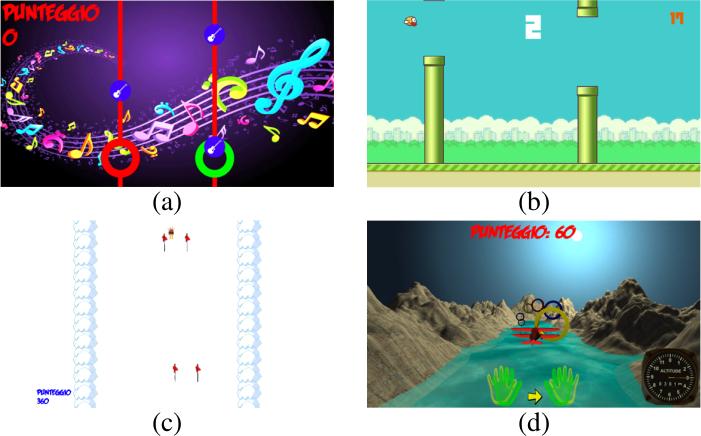
\includegraphics[scale=0.5]{./img/corona_games.png}}
\end{figure}

Para interação com os jogos foi utilizado o dispositivo LMP, este permite a deteção de vários pontos da mão.
Foram realizadas validações preliminares com 6 participantes (com idades compreendidas entre os 10 e os 21 anos) na Clínica Pediátrica \textit{G. e D. De Marchi} e
receberam feedback positivo quer dos pacientes, quer dos terapeutas.\\

A empresa \textit{Rehability} (\url{www.rehability.me}) dedica-se ao desenvolvimento de jogos para reabilitação física e cognitiva.
Ao utilizar a estratégia User Centered Design (UCD), desenvolvendo os jogos em conjunto com os seus pacientes, permite que estes sejam muito
mais focados nas necessidades dos mesmos. Contam com várias publicações científicas nesta área e 6 prémios.
Os jogos e técnicas desenvolvidos por esta empresa são bastante avançados e serviram de inspiração para o desenvolvimento dos nossos.

\subsection{Reconhecimento de Gestos}

\subsubsection{Software}

Na tese de licenciatura \cite{poznan} os autores desenvolveram uma biblioteca em C++ para aprender e reconhecer gestos estáticos e dinâmicos usando o LMC.
O algoritmo utilizado para aprender a reconhecer gestos estáticos foi o \textit{Support Vector Machine} (SVM).
O SVM é um modelo de aprendizagem não supervisionada que tenta encontrar o hiperplano que maximiza a margem entre as classes pretendidas (Ver Figura \ref{fig:svm}).

\begin{figure}[h!]
    \center
    \includegraphics[scale=1.2]{./img/svm.png}
    \caption{Adaptado de: \\ \url{https://cdn-images-1.medium.com/max/1600/1*nUpw5agP-Vefm4Uinteq-A.png}.}
    \label{fig:svm}
\end{figure}

Para testar o algoritmo foram utilizados os seguintes gestos (ver Figura \ref{fig:10_gestures}):

\begin{figure}[h!]
    \center
    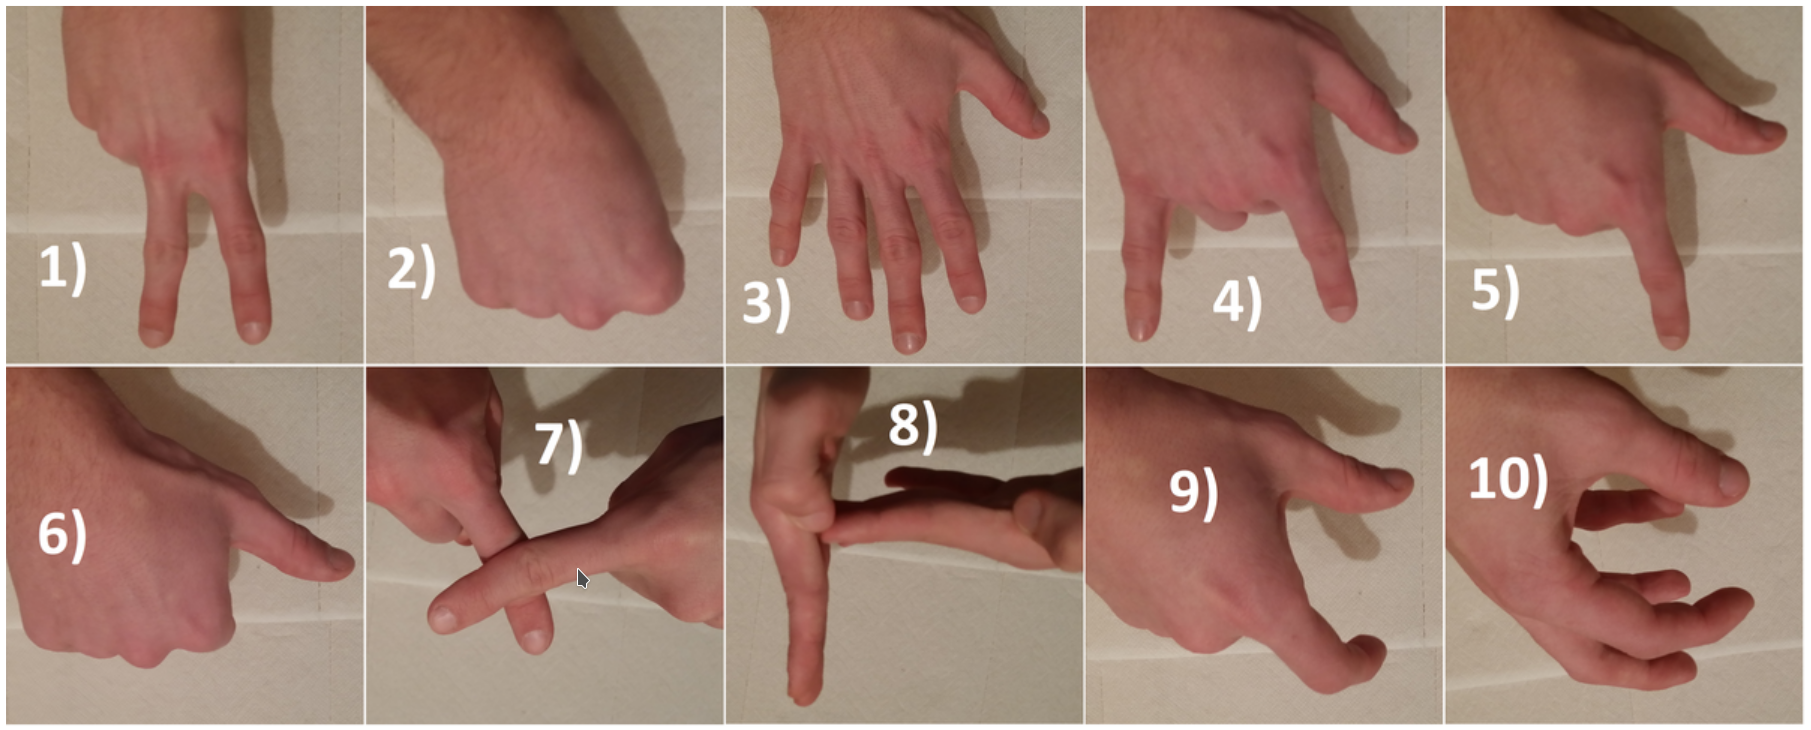
\includegraphics[scale=0.25]{./img/10_gestures.png}
    \caption{Dez gestos utilizados para testar o algoritmo proposto.}
    \label{fig:10_gestures}
\end{figure}

No total foram capturados 5000 amostras para cada classe (gesto), 1000 por cada autor.
Para treino e teste os dados foram divididos numa relação de 2 para 1 e para validar a performance do modelo,
utilizaram o \textit{k-fold cross validation}, que consiste em dividir aleatoriamente o dataset em k grupos
de tamanho aproximadamente igual, o primeiro grupo é usada para validar o modelo e os restantes para treinar o mesmo.

Eles realizaram testes usando as seguintes \textit{features}:
\begin{itemize}
    \item \tetxit{Feature vector} 1: Número de dedos estendidos, distância euclidiana entre as pontas dos dedos consecutivos e o ângulo absoluto entre dedos consecutivos.
    \item \tetxit{Feature vector} 2: \textit{Feature vector} 1 e as distâncias entre pontas de dedos consecutivas e a posição da palma da mão.
    \item \tetxit{Feature vector} 3: \textit{Feature vector} 2 e os cinco ângulos entre dedos e o vetor normal da palma da mão.
    \item \tetxit{Feature vector} 4, 5 e 6: \textit{Feature vector} 1, 2 e 3 respetivamente, mas invés das distâncias e ângulos absolutos contém os cinco valores
                  mais elevados das distâncias e dos ângulos entre todas as combinações possíveis dos dedos.
\end{itemize}

Os melhores resultados foram obtidos utilizando o \textit{Feature vector} 6:
\begin{center}
    \begin{tabular}{|p{2.1cm}|p{2.7cm}|p{2.3cm}|p{2.8cm}|}
        \hline
        5 gestos (CV) & 5 gestos (Conjunto de teste) & 10 gestos (CV) & 10 gestos (Conjunto de teste) \\
        \hline
        \hline
        92.8\% & 93.1\% & 80.5\% & 81.2\% \\
        \hline
    \end{tabular}
\end{center}

No artigo \cite{mit} os autores desenvolveram uma biblioteca \textit{open source} em C++ para reconhecer gestos em tempo real.
A biblioteca tem a funcionalidade para usar um vasto número de algoritmos de \textit{machine learning} como \textit{Decision Trees},
\textit{Hidden Markov Models}, \textit{K-Nearest Neighbor}, \textit{Linear} e \textit{Logistic Regression}, \textit{Naı̈ve Bayes},
\textit{Support Vector Machines}, \textit{et cetera}.
Este artigo não é relevante para a parte de desenvolvimento pois não possui qualquer tipo de explicação em relação aos métodos usados,
no entanto fornece uma base de comparação para a qualidade da nossa solução.


No artigo \cite{handGestureReconWithLMC} os autores criaram um dataset de amostra colhidas através do LMC que é composto por
por um total de 2600 amostras: 10 gestos repetidos 20 vezes por 13 pessoas diferentes.

Para entrada dos modelos utilizaram as seguintes \textit{features}:

\begin{itemize}
    \item Ângulo entre as pontas dos dedos ($A$):

    \begin{equation}
        A_i = \angle(F_i^\pi - C, h)
    \end{equation}

    \begin{itemize}
        \item $F_i^\pi$ : Projeção das coordenadas da ponta do dedo no índice $i$ no plano, determinado pelo vetor direção perpendicular ao plano da palma da mão.
        \item $C$ : Coordenadas no espaço 3D do centro da palma da mão em relação ao LMC.
        \item $h$ : Vetor com as direções entre a o centro da palma da mão e os dedos.
    \end{itemize}

    \item Distância entra a palma e a ponta dos dedos ($D$):

    \begin{equation}
        D_i = \frac{\mid\mid F_i - C \mid\mid}{F_{middle} - C}
    \end{equation}

    \begin{itemize}
        \item $F_i$ : Coordenadas no espaço 3D da ponta do dedo no índice $i$.
        \item $F_{middle}$ : Coordenadas no espaço 3D da ponta do dedo do meio.
    \end{itemize}

    \item Elevação da ponta dos dedos ($E$):

    \begin{equation}
        E_i = \frac{\sin((F_i - F_i^\pi)*n)*\mid\mid F_i - F_i^\pi \mid\mid}{F_{middle} - C}
    \end{equation}

    \begin{itemize}
        \item $n$ : Vetor direção perpendicular ao plano da palma da mão.
    \end{itemize}

    \item Distância entre as pontas de dedos adjacentes ($T$):

    \begin{equation}
        T_{ij} = \frac{\mid\mid F_i - F_j \mid\mid}{F_{middle} - C}, 1 \le i \ne j \le 5
    \end{equation}

    \item \textit{Histogram of oriented gradients} (HOG):
    \begin{itemize}
        \item HOG é um descritor de características cujo objetivo é generalizar um objeto de maneira tal que o mesmo objeto
              produza descritores de características o mais semelhantes possíveis quando visto sobre condições diferentes.
    \end{itemize}
\end{itemize}

Algoritmo usado foi o SVM com uma estratégia \textit{One-vs-One} para classificação multi-classe, de um total de 10 classes.
A estratégia \textit{One-vs-One} consiste em treinar $n * (n-1) / 2$ classificadores binários, neste caso $n = 10$ resulta em 45 classificadores.
Uma amostra é classificada por todos os classificadores e a classe com mais votos ganha e a amostra é classificada como sendo dessa classe.

A melhor precisão que obtiveram com o dataset criado foi de 99.42\%.

\subsubsection{Hardware}

No artigo \cite{linshao} foi nos possível adquirir várias informações sobre o hardware LMC.
O dispositivo LMC possui uma dimensão de $1.3$x$3.0$x$8.0$ cm, para o utilizador poder interagir com o dispositivo
tem de o conectar por USB ao seu computador ter instalado o SDK do Leap Motion.

De acordo com este artigo, o LMC fornece uma precisão de deteção de cerca de 200\texit{\mu m}.

Para avaliar a performance do dispositivo, este foi comparado com um rato comum, tendo em conta a lei de Fitts, a performance
do LMC em tarefas gerais que envolvem apontar num computador foi inferior, com uma taxa de erro de 7.81\%, quando comparada com o rato,
com uma taxa de erro de 2.8\%.
Por outro lado o LMC permite ao utilizador usar o disposito sem nenhum tipo de restrições físicas, pois apenas é necessário colocar a(s)
mão(s) por cima do dispositivo, sem ser necessária a utilização de elementos adicionais, como luvas e entre outros.

O dispositivo é composto por três emissores infravermelhos e duas câmeras que recebem raios infravermelhos (ver figura \ref{fig:lmc}).

\begin{figure}[h!]
    \center
    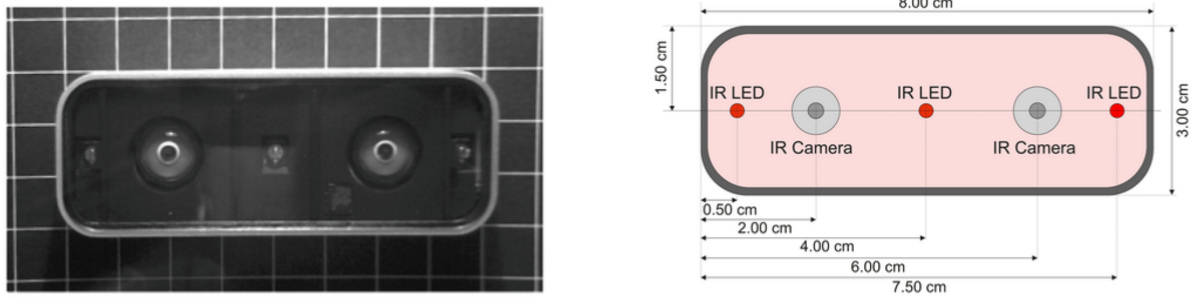
\includegraphics[scale=0.4]{./img/lmc.png}
    \caption{Estrutura interna do LMC. Adaptado do artigo \cite{linshao}.}
    \label{fig:lmc}
\end{figure}

\newpage

Através do SDK é possível obter informação sobre:

\begin{itemize}
    \item Posição do centro da palma da mão, e o vetor normal à mesma.
    \item Direção da Mão.
    \item Posição da ponta dos dedos (coordenadas 3D), direção e velocidade dos dedos.
    \item Direção do braço.
\end{itemize}

Sendo que os valores estão em milímetros.

%Neste relatório o autor utilizou a API do LMC para reconhecer movimentos e gestos estáticos.
%
%As \textit{features} utilizadas foram:
%\begin{itemize}
%    \item Distance between fingertips and palm center.
%    \item Distance between two fingers which are adjacent.
%\end{itemize}
%
%O autor definiu manualmente a deteção de gestos de acordo com as features.
%
%Trabalho um pouco pobre no que toca a reconhecimento de gestos mas revela alguns promenores sobre problemas do LMC.

\section{Modelo Conceptual}

\subsection{Requisitos do Sistema}

Esta secção apresenta e especificação do sistema resultante da primeira fase de prototipagem.

\subsubsection{Obtenção de Requisitos}

A obtenção de requísitos foi caracterizada por três fases.
A primeira fase foi a avaliação dos objetivos do sistema,
realizada numa conversa informal com o nosso orientador Sérgio Matos,
que permitiu restringir a abrangência do mesmo. Definimos nesta fase o nosso público alvo e a nossa área de atuação.
A segunda fase foi a procura do estado da arte, que consiste na procura por artigos, teses,
projetos e tecnologias semelhantes, nesta fase encontramos alguns artigos que nos revelaram as
vantagens/desvantagens de várias abordagens. Após esta análise definimos as tecnologias a usar.
A terceira e a última fase foi o contacto com os clientes do sistema, médicos (especialidade),
que nos dá uma visão do que é esperado do mesmo, permitindo a extração de requisitos funcionais e não funcionais.

Depois de analisadas todas as opções as seguintes decisões foram tomadas:

\begin{itemize}
    \item O sistema contaria com duas interfaces, uma para o paciente e uma para o médico.
          Isto deve-se aos objetivos e o ambiente de utilização serem distintos.
          O médico usaria a sua interface num computador do hospital
          durante uma consulta enquanto o utente usaria a sua interface em qualquer computador em casa durante o tratamento.
    \item Dada a heterogeniedade de utentes que podem sofrer de artrites a interface direcionada ao paciente teria de ser clara,
          intuítiva e focada. Sendo que por isso optamos por uma interface gráfica onde os menus seriam grandes e com pouca informação.
          Permitindo até ao utilizador mais idoso entender a interface.
    \item A interface destinada aos médicos seria esta também gráfica, dada a baixa formação informática dos mesmos,
          e devia contar com uma área dedicada à análise da evolução dos pacientes, permitir a adição de novos gestos
          sem necessidade de adição de código e também devia permitir a adição de novos pacientes.
    \item Uma vez que os jogos teriam de ser jogados usando o leap motion estes teriam de ser simples e fáceis de aprender.
          Como o objetivo era também lembrar os jogos mais antigos estes seguiriam o estilo arcade. Uma vez que o tratamento das
          artrites consiste na repetição de um mesmo movimento repetidamente cada jogo é apenas jogado com um movimento de cada vez,
          permitindo realizar as repetições necessárias.
    \item Para que fosse possível uma maior liberdade na escolha do gesto a jogar em cada jogo foi também definido que existiria um
          middleware entre o jogo e o leap motion que faria a verificação do gesto realizado para o movimento acontecer no jogo.
          Permitindo que qualquer jogo fosse jogado com qualquer movimento e até o desenvolvimento de novas deteções de movimento ou jogos sem grandes alterações.
\end{itemize}

\subsubsection{Descrição do Contexto de Utilização}

Nesta secção abordaremos a forma como esperamos que o sistema seja utilizado pelos stakeholders.
Começando pelo médico chefe este é responsável pela gestão dos médicos.
Deverá fazer a inscrição/remoção dos médicos, e poderá ainda supervisionar todos os pacientes, caso seja necessário uma segunda opinião.

Após a inscrição de um médico na plataforma este poderá utilizar a plataforma realizando login.
Sempre que receber um novo paciente, este deve inscrevê-lo no sistema (operação rápida de 1 ou 2 minutos) para que este depois possa utilizar o sistema.
Como ferramenta de auxílio durante o tratamento o médico pode seguir o progresso dos pacientes inscritos acedendo aos gráficos estatísticos destes.
Se o médico desejar pode ainda deixar notas para o paciente ou privadas como forma de comunicar informações importantes

Um paciente após ser inscrito pelo médico, irá receber um email com as credenciais.
Depois de realizar login com essas credenciais este será encaminhado para a página de jogos, onde escolherá um jogo e um dos movimentos,
começando depois o jogo e assim o tratamento. Caso o paciente deseje ver as métricas de progressão do seu tratamento,
este poderá dirigir-se à página de estatísticas e ver a sua evolução. É ainda possível que o médico deixe notas ao paciente, que este visualizará na página de perfil.

\subsubsection{Atores}

O público alvo da nossa aplicação é muito variado uma vez que as artrites podem aparecer em qualquer faixa etária.
 Sendo que para a utilização da aplicação será apenas necessário o conhecimento
básico de utlização de um computador. O utilizador da aplicação web será um médico pelo que contamos com alguma experiência
de utilização de computadores e sistemas de gestão. Contudo qualquer pessoa com alguma experiência de navegação na web será capaz de utilizar o sistema.

Os atores do sistema estão apresentados na lista a baixo:

\begin{itemize}
    \item Paciente: Representa todos os pacientes, sendo a maioria dos utilizadores do sistema.
          Têm acesso apenas à aplicação desktop e nesta podem jogar os jogos, ver as notas do médico e a sua progressão.
    \item Médico: Utilizador da aplicação web responsável pela adição de novos pacientes e gestos para
		  os mesmos ao sistema e posteriormente da sua monitorização.
	\item Médico chefe: Utilizador da aplicação web reponsável pela adição/remoção de fisatras,
		  podendo realizar para além disso todas as funções de um fisiatra normal.
\end{itemize}

\subsubsection{Casos de Uso}

Na figura \ref{fig:use_case} é possível visualizar os casos de uso do nosso sistema.
Estes são divididos em dois conjuntos: o conjunto da aplicação do paciente e o conjunto da aplicação do médico.
Que representam o uso da aplicação desktop e web respetivamente.

\begin{figure}[h!]
    \center
    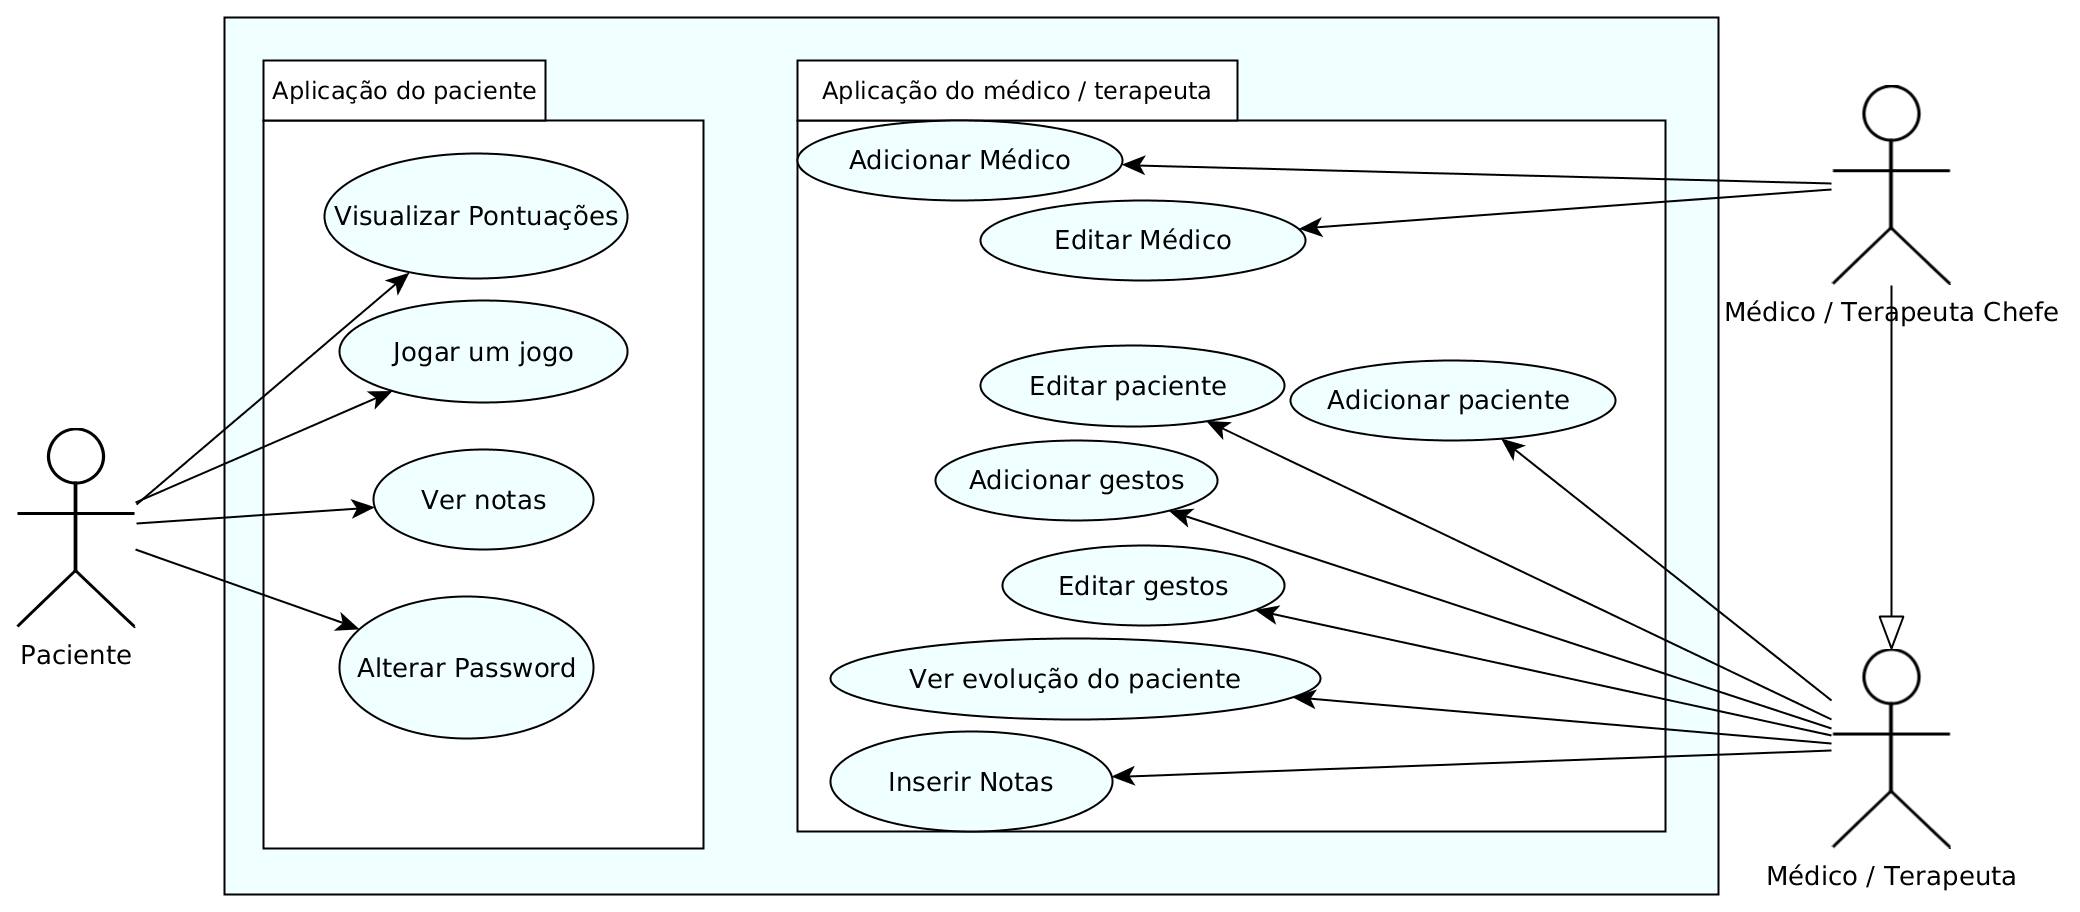
\includegraphics[scale=0.17]{./img/use_case.jpg}
    \caption{Diagrama dos casos de uso.}
    \label{fig:use_case}
\end{figure}

\newpage

Descrição dos casos de uso:

\textbf{Casos de uso do paciente:}
\begin{itemize}
	\item Visualizar Pontuações: Permite que o paciente veja gráficamente o seu progresso.
		  É suposto que o paciente já tenha jogado alguns jogos, para que as métricas a mostrar tenham valores.
		  O paciente pode visualizar as pontuações que obteve nos jogos e o número de gestos corretamente e incorretamente realizados.\\
          Prioridade : Alta.
	\item Jogar um jogo: Permite ao paciente jogar diferentes jogos, com recurso a um dos movimentos disponíveis.
		  É suposto que o paciente juntamente com o médico tenham treinado pelo menos um gesto a ser realizado.
          Quando abre esta opção o paciente vê uma lista de jogos que pode escolher, tendo que de seguida escolher o gesto e por fim jogar.\\
          Prioridade: Alta.
	\item Ver notas: O paciente antes de jogar pode dirigir-se ao seu perfíl para verficar as notas que o médico deixou.\\
		  Prioridade: Média.
	\item Alterar a Password: Permite que o paciente altere a password.
		  Esta é uma funcionalidade de relevância uma vez que a primeira password é gerada aleatoriamente.\\
		  Prioridade: Média
\end{itemize}

\textbf{Casos de Uso do Médico:}
\begin{itemize}
	\item Adicionar Paciente: Sempre que um novo paciente é atribuído a um médico este
		  deve registá-lo na plataforma preenchendo os dados pessoais do mesmo.
		  É um processo rápido de 2 minutos onde o médico preenche apenas os dados necessários para identificar o paciente.\\
          Prioridade: Alta.
	\item Editar Paciente: Engloba a edição e remoção de um paciente.
		  Caso um médico se engane no preenchimento de algum dado ou o paciente não seja necessário no sistema o médico pode editar os dados ou mesmo eliminá-los.\\
          Prioridade: Alta.
	\item Adicionar Gesto: Para que o paciente possa jogar os jogos este necessita de ter gestos definidos.
		  Com esse objetivo, o médico durante uma consulta usa o sistema para adicionar um gesto ao paciente.
		  A adição do gesto é um processo com um tempo inferior 1 minuto.\\
          Prioridade: Alta.
	\item Editar Gesto: Com a evolução um paciente torna-se mais apto a realizar um movimento o que pode causar erros na deteção do mesmo.
		  Nessas situações cabe ao médico editar o gesto juntamente com o paciente, para que volte a funcionar corretamente.\\
	      Prioridade: Alta.
	\item Ver Evolução de um Paciente: O médico após realizar a inscrição de um paciente na plataforma e este jogar alguns jogos,
		  pode ver a evolução do mesmo. Quando entra nesta aba pode observar o número de movimentos corretos, errados, as
		  pontuações nos jogos e a dificuldade em que este o jogou.\\
		  Prioridade: Alta.
	\item Inserir Notas: Para relembrar o paciente ou até para se lembrar mais tarde, o médico pode inserir notas privadas (só para o médico)
		  ou partilhadas (com o paciente). Isto permite um contacto mais próximo com um paciente sem necessidade de consultas.\\
		  Prioridade: Média.
\end{itemize}

\textbf{Casos de Uso do Médico Chefe:}
\begin{itemize}
	\item Adicionar Médico: Sempre que um novo profissional é contratado este é inscrito no sistema pelo responsável (médico chefe)
		  do sistema, preenchendo os seus dados pessoais. Este processo é bastante semelhante à inscrição de um paciente, sendo também um processo de 2 minutos.
	\item Editar Médico: Caso ocorra algum engano durante o preenchimento do campos de inscrição de um médico ou um médico
		  não seja necessário no sistema, o médico chefe pode editar os campos ou mesmo remover o médico.
\end{itemize}


% DESCREVER O PROBLEMA.
% REQUISITOS.
% TERMINOLOGIA.
% EVITAR DETALHES DE IMPLEMENTAÇÃO.

\section{Pesquisa}

\subsection{Reconhecimento de Gestosi Através do LMC}

Para o reconhecimento de gestos criamos um \textit{dataset} com 4 gestos, cada um com 500 amostras do gesto correto e outras 500
com gestos diferentes do pretendido. Depois de alguns testes e uma análise detalhada de todas as \tetxit{features} utilizadas pelos outros autores,
concluímos que as mais adequadas ao nosso problema eram as seguintes:

\begin{itemize}
    \item Distância normalizada entre a ponta dos dedos adjacentes:
    \begin{equation}
        \forall_{i,j} \quad D_{i,j} = \frac{(F_j - F_i) - \min \{D_{i,j}\}}{\max \{D_{i,j}\} - \min \{D_{i,j}\}}, \quad 1 \le i \ne j \le 5
    \end{equation}
        \begin{itemize}
            \item $i, j$ : Índices dos dedos.
            \item $F_i$ : Posição da ponta do dedo (fingertip) do dedo com o índice $i$.
        \end{itemize}
    \item Número de dedos estendidos (informação fornecida pela API do LMC).
\end{itemize}

Para determinar qual o modelo mais adequado a este contexto utilizamos as amostras do gesto da mão fechada (ver figura \ref{fig:closed_hand}),
treinamos e validamos 9 modelos de machine learning, os dados foram divididos da seguinta forma: 80\% para treino e 20\% para teste,
e os resultados foram os seguintes:

\begin{table}[h!]
    \center
    \begin{tabular}{|l|c|r|}
        \hline
        \textbf{Modelo} & \textbf{Precisão (\%)} & \textbf{\textit{Runtime} (ms)}\\
        \hline
        \hline
        Naive Bayes & 96.15 & 1728\\
        Generalized Linear Model & 95.10 & 6140\\
        Logistic Regression & 95.79 & 1178\\
        Fast Large Margin & 95.45 & 1255\\
        Deep Learning & 96.84 & 6873\\
        \textbf{Decision Tree} & \textbf{98.75} & \textbf{101}\\
        Random Forest & 98.56 & 6922\\
        Gradient Boosted Trees & 98.59 & 23265\\
        Support Vector Machine & 98.51 & 2403\\
        \hline
    \end{tabular}
    \caption{Resultados dos vários modelos utilizados para reconhecer o gesto da mão fechada.}
\end{table}

\vspace{-0.45cm}

\begin{figure}[h!]
    \center
    \frame{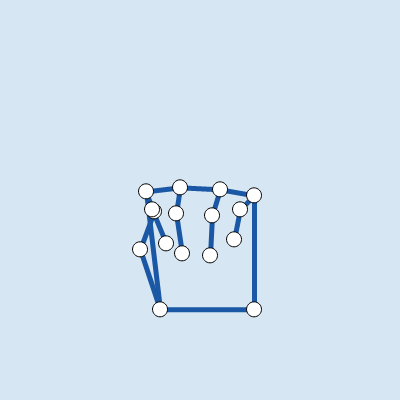
\includegraphics[scale=0.35]{./img/closed_hand.png}}
    \caption{Amostra recolhida pelo LMC do gesto da mão fechada.}
    \label{fig:closed_hand}
\end{figure}

Como podemos observar pela tabela acima obtivemos os melhores resultados para o algoritmo árvore de decisão, sende este também o mais rápido.
Uma vantagem deste modelo é este também ser bastante leve em termos de memória, uma árvore de decisão pode ser representada como uma estrutura de dados
recursiva e quando guardada em formato JSON, por exemplo, ocupa entre 1k a 5k em disco.

Podemos observar o processo completo de reconhecimento de um gesto no diagrama da figura \ref{fig:ml_model}.

\begin{figure}[h!]
    \center
    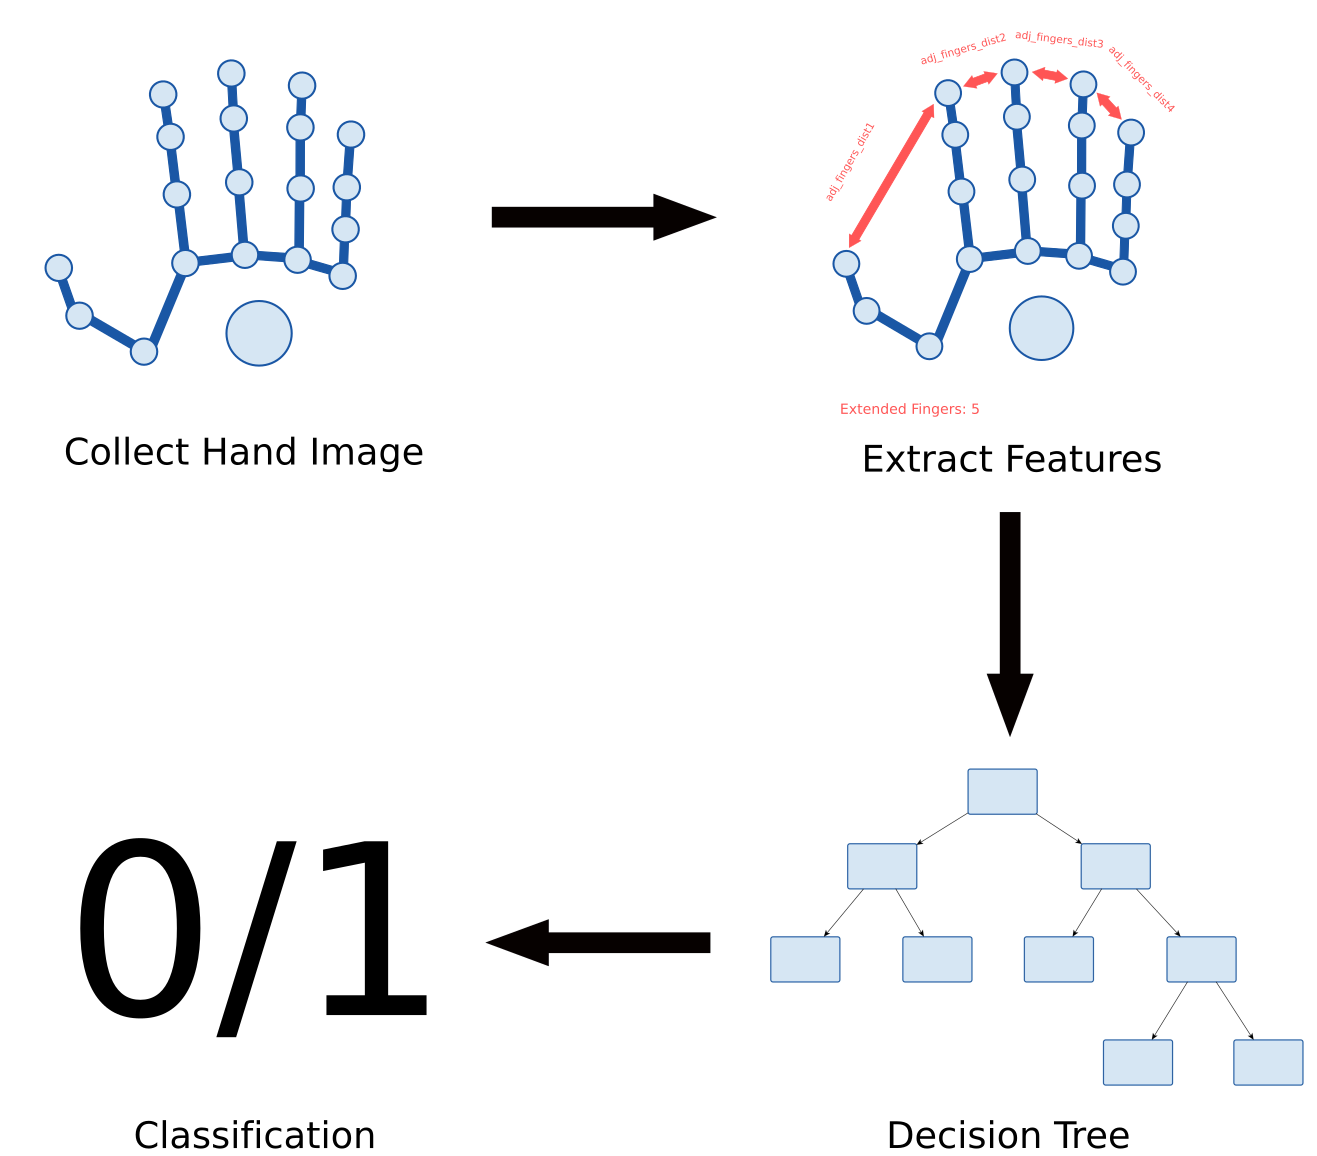
\includegraphics[scale=0.3]{./img/ml_model.png}
    \caption{Processo completo do reconhecimento de gestos.}
    \label{fig:ml_model}
\end{figure}

No entanto, para construir um sistema onde sejam necessários reconhecer vários gestos, uma árvore de decisão não chega, temos de possuir várias, uma para
cada gesto, faltando ainda definir um método para unir o conhecimento das várias árvores para obter uma classificação final.

Existem várias estratégias para realizar \textit{multiclass classification}, como \textit{One vs. All} ou \textit{One vs. One}, no entanto para aplicar este tipo
de estratégia é necessário que os modelos utiliados retornem um nível de confiança em relação à sua classificação (\textit{e.g.} retornar um número pertencente ao conjunto: $\{x \in \mathbb{R} \mid 0 \le x \le 1\}$), o que não acontece com as árvores de decisão,
apenas retornam a classificação em si, 1 ou 0, sim ou não.

Como tal decidimos adotar uma estratégia mais simples, onde percorremos as árvores (cada árvore representa um gesto) por uma ordem qualquer, e a primeira que retornar 1
faz com que a amostra seja classificada com gesto associado a essa árvore.

\vspace{0.2cm}
\begin{figure}[h!]
    \center
    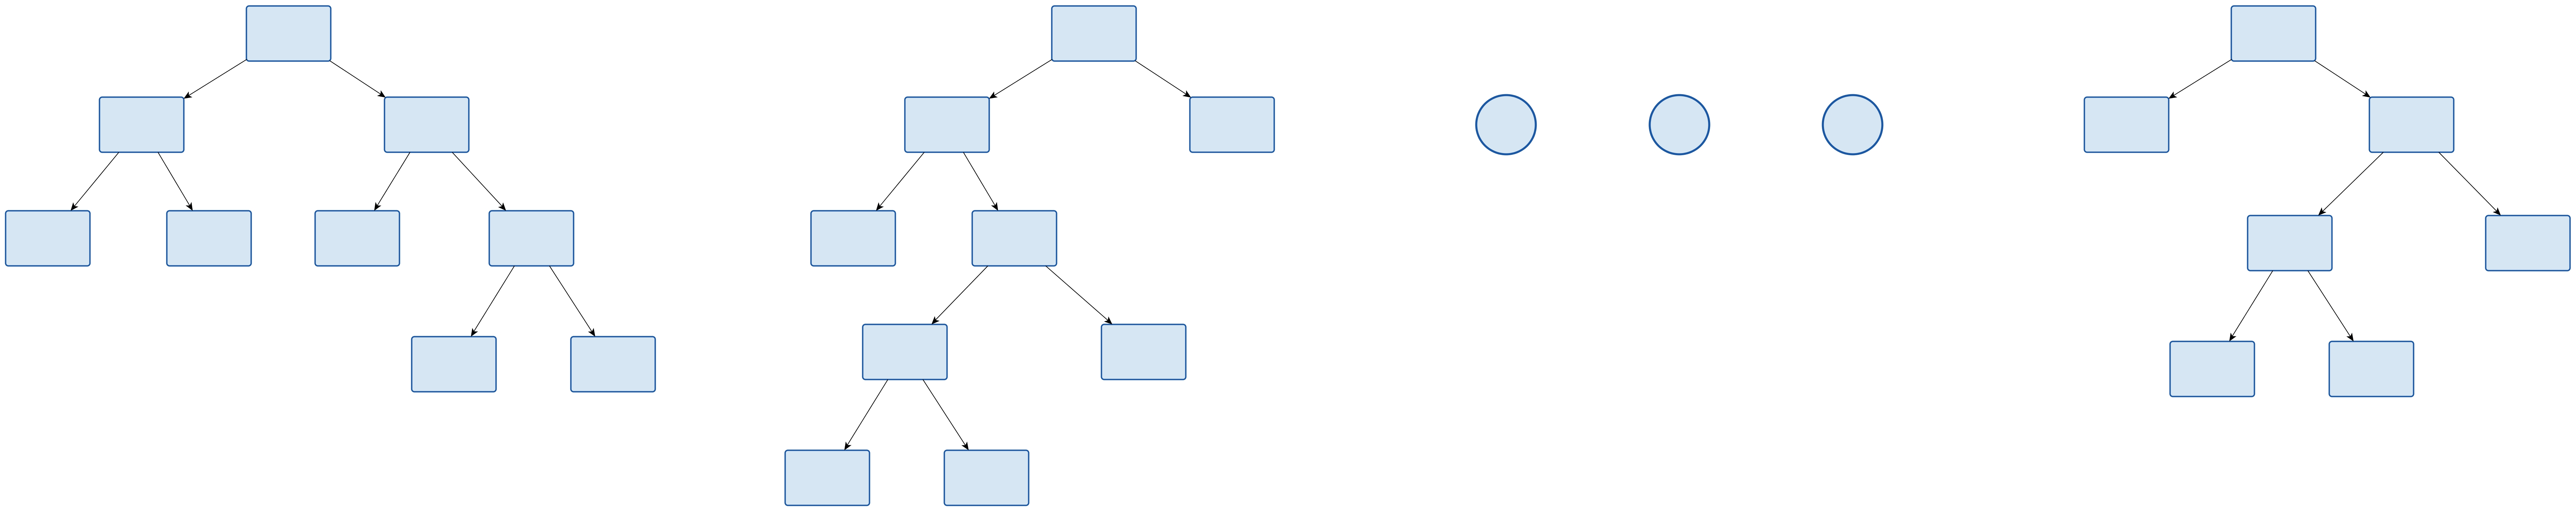
\includegraphics[scale=0.04]{./img/multiclass_classification.jpg}
    \vspace{0.2cm}
    \caption{Visualização do método adotado para realizar \textit{multiclass classification}.}
    \label{fig:multiclass}
\end{figure}

Para validar a eficácia do método descrito realizamos um teste com 4 gestos (mão aberta, mão fechada, símbolo da paz e a letra \textbf{Y} em linguagem gestual portuguesa,
ver figura \ref{fig:heat_map}).
Foram treinadas 4 árvores de decisão cada uma com 1000 amostras, 500 amostras do gesto correto, 500 amostras de outros gestos que não o correto.
Os resultados estão presentos no seguinte mapa de calor (ver figura \ref{fig:heat_map}):

\begin{figure}[h!]
    \center
    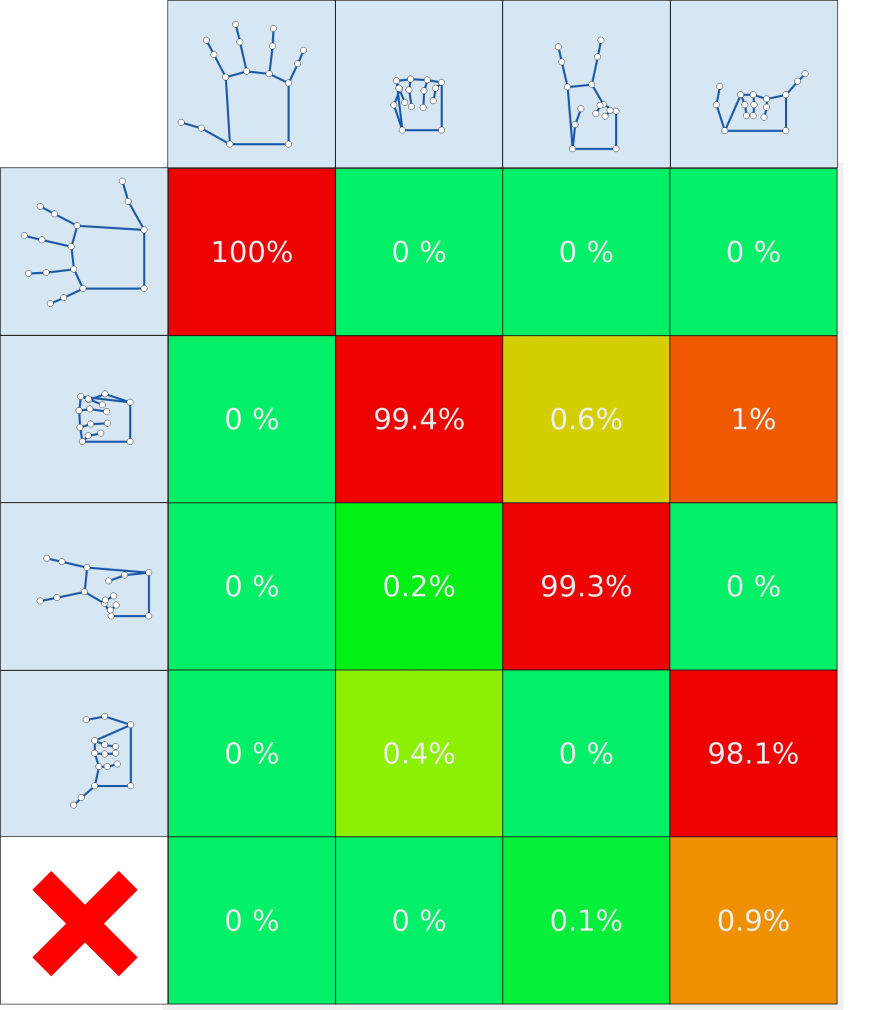
\includegraphics[scale=0.3]{./img/heat_map.png}
    \caption{Resultados da validação do método para \textit{multiclass classification}.}
    \label{fig:heat_map}
\end{figure}

Através do mapa de calor é possível observar, como esperado, que a precisão de reconhecimento do gestos vai diminuindo consoante a posição do gesto. Considerando
que as árvores de decisão estão num \textit{array}, o gesto associado à árvore que estiver na última posição vai ser o que terá piores resultados, dado que há um maior
número de árvores de decisão para trás, e portanto uma maior probabilidade de o gesto ser mal reconhecido.

Ainda assim, consideramos que os resultados são bastante satisfatórios, até porque nunca serão utilizados mais do que dois gestos ao mesmo tempo. Pois tendo em conta
os requisitos obtidos junto dos médicos o paciente terá de realizar o mesmo gesto repetidamente. Como tal, seram utilizadas apenas as árvores correspondentes à mão aberta
e ao gesto em questão, a árvore de decisão relativa à mão aberta irá servir para saber se o paciente realizou o gesto completo, isto é, estava com a mão aberta,
realizou o gesto pretendido e voltou à posição da mão aberta. Esta estratégia também irá permitir saber se o paciente não conseguiu realizar o gesto, pois se este está
com a mão aberta e de seguida deixa de estar com a mão aberta mas também não realiza o gesto pretendido e volta a abrir a mão, então é porque este tentou realizar o gesto
pretendido, mas não conseguiu flexionar a mão totalmente, resultando num gesto mal realizado. Para além de detetar gestos mal realizados também nos permite saber quanto
tempo demorou o paciente a realizar o gesto.

\subsection{Reconhecimento de gestos através de um dispositivo Android.}

\subsubsection{Objetivos}

A recolha de gestos através de um dispositivo Android tem como motivação o facto de permitir aos pacientes realizarem o seu tratamento a partir da
comodidade do seu lar, sem terem que se deslocar a um hospital para realizar reabilitação.

Desta forma, iniciou-se um processo de pesquisa que permitisse avaliar se esta funcionalidade poderia, de facto, ser aplicada ao nosso sistema.
Recorremos, então, ao SDK do OpenCv para Android.

\subsubsection{OpenCV}

O OpenCV (Open Source Computer Vision Library)  é um software open source de visão por computador.
Esta biblioteca contém inúmeros algoritmos de machine learning para reconhecer determinados elementos numa imagem recolhida.

Utilizámos o SDK fornecido pelo OpenCV para Android, sendo que rapidamente foi possível observar que o mesmo se encontra pouco desenvolvido, sendo, portanto, bastante limitativo.

\subsubsection{Recolha e Análise de Imagens}

Tendo adquirido diversos frames através da câmera do dispositivo Android, estes eram transpostos para matrizes RGB, representativas do frame em questão.

Posteriormente, o utilizador, selecionava (carregava sobre) um ponto da imagem que estivesse dentro do contorno da sua mão.
Para tal, foi necessário converter a localização (em pixéis) do ponto que o utilizador selecionou para a localização do seu correspondente na imagem recolhida.
Após isto, com recurso ao cálculo de um desvio padrão associado à cor do pixel que o utilizador selecionou, é calculado e desenhado o contorno da mão do mesmo.
De forma a facilitar este processo, o utilizador poderia recorrer a uma luva de látex com uma cor diferente daquela do ambiente que o rodeia -
por exemplo, uma luva roxa. Após investigação, concluímos que este era o método aconselhado pela maioria dos developers que experienciaram o mesmo desafio.

Depois do reconhecimento do contorno da mão, procedemos ao reconhecimento das pontas dos dedos e dos pontos extremos dos vales inter-dedos.
Conseguimos, também, identificar o centro de massa da mão do utente, o que, tendo em conta os ângulos entre as pontas dos dedos identificados,
poderia ser utilizado para identificar individualmente cada dedo. Poderíamos, por exemplo, determinar se o utilizador tinha o dedo indicador em extensão ou flexão.

\begin{figure}[h!]
    \center
    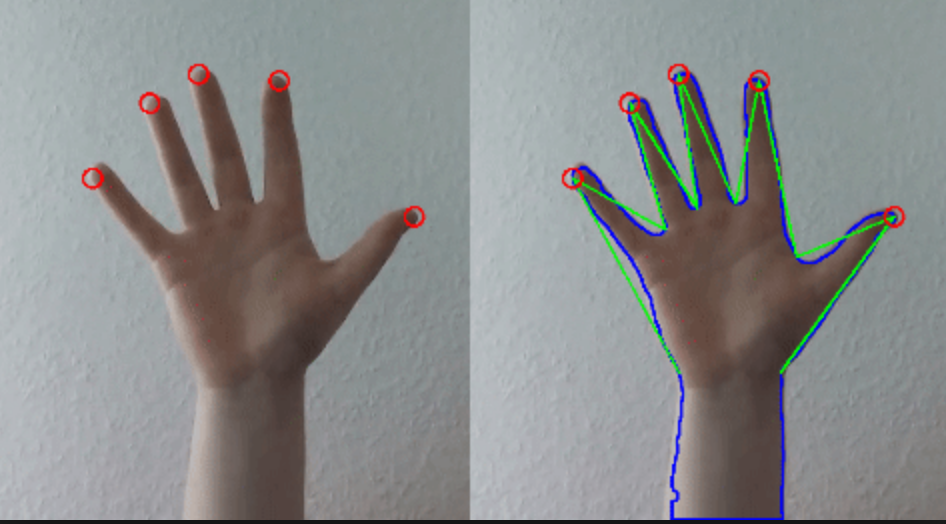
\includegraphics[scale=0.5]{./img/opencv1.png}
    \caption{Reconhecimento das bordas de uma mão usando OpenCV em android.}
    \label{fig:opencv1}
\end{figure}

Foi nesta etapa que observámos que o dispositivo Android estava com alguma latência em obter imagens e a extrair features das mesmas.

\subsubsection{Problemas Encontrados}

Tal como mencionado acima, o dispositivo Android demorava um elevado período de tempo a reconhecer as features das imagens que estavam a ser obtidas.

Para tentar colmatar este problema, reduzimos a resolução das imagens obtidas, tendo-se notado uma melhoria significativa.
A baixas resoluções, a capacidade de processamento de um dispositivo Android é suficiente para analisar os frames recolhidos.

Contudo, surgiu um problema inerente à baixa resolução da recolha de imagens. Uma vez que os frames tinha uma resolução muito baixa,
era bastante difícil reconhecer as features em causa com a precisão necessária para avaliar a correção de um gesto a ser utilizado para reabilitação de um paciente com artrite.

\begin{figure}[h!]
    \center
    \frame{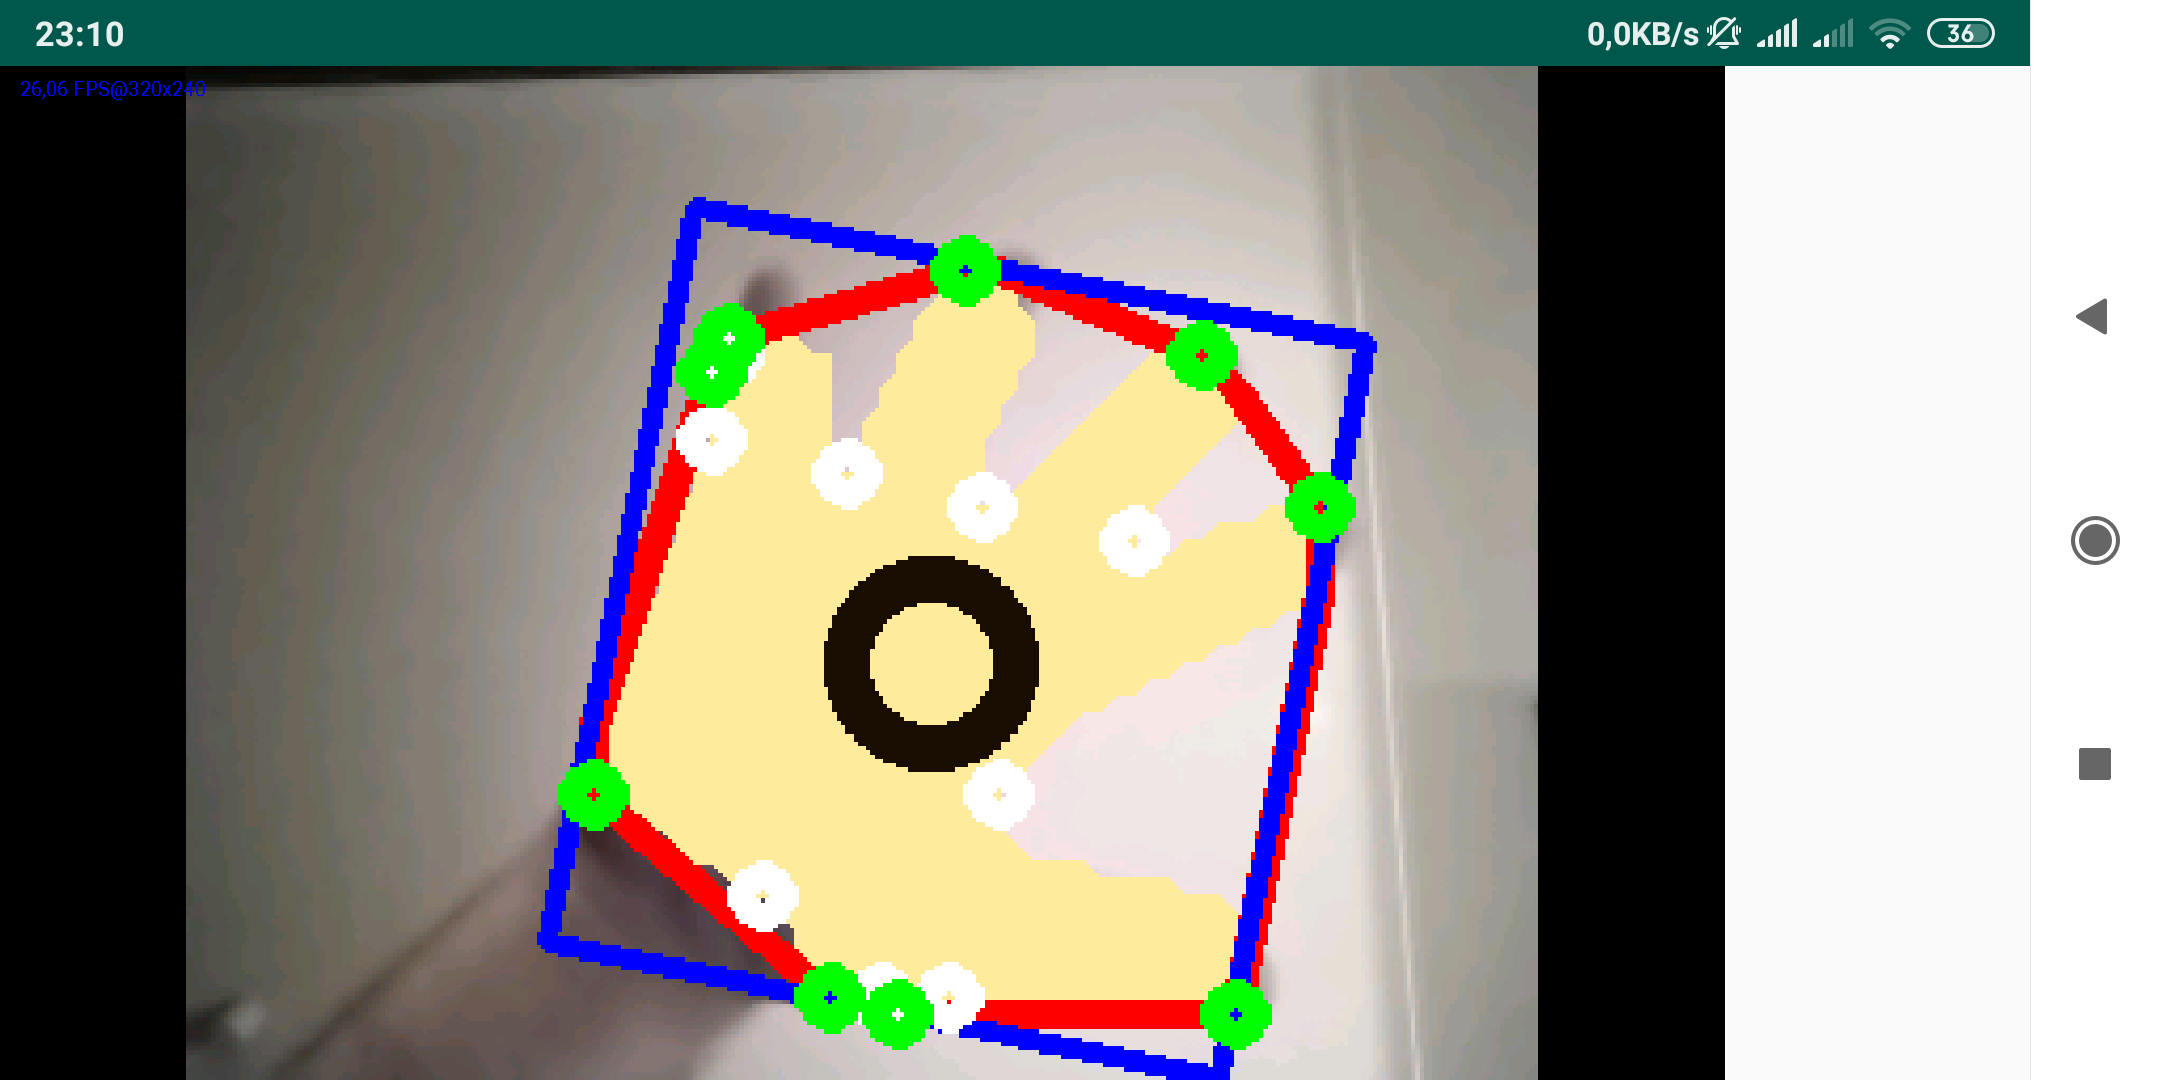
\includegraphics[scale=0.15]{./img/opencv2.png}}
    \caption{Reconhecimento da área da mão.}
    \label{fig:opencv2}
\end{figure}

Após isto, consultámos, durante uma conversa informal, um professor da Universidade de Aveiro bastante experiente na área de visão por computador
que nos informou que o reconhecimento de features que desejávamos realizar poderia não ser, de todo, exequível de realizar num dispositivo Android.
Aconselhou-nos a realizar este processamento num processo remoto. Esta opção, infelizmente, não pode ser utilizada no nosso sistema, uma vez que o
envio de um frame para análise num processo remoto introduz uma elevada latência ao jogo no qual se encontra o paciente. Para que o paciente consiga
jogar um serious game através de gestos, a sua recolha e análise tem de ser feita em real time, algo que não é possível de obter com uma extração de
remota de features de um frame.

\subsubsection{Conclusão}

Apesar de ser uma funcionalidade extraordinária para os utilizadores da nossa plataforma, concluímos que a tecnologia existente na atualidade
ainda não é suficiente para realizar o que pretendíamos. Optámos, então, por recolher e analisar os gestos somente através do Leap Motion.

\section{Procedimento}

\subsection{Arquitetura do Sistema}

O sistema possui 3 componentes principais: a aplicação do médico, a do paciente e o servidor de gestão, que contém a REST API e base de dados.

No diagrama de instalação (figura \ref{fig:deployment}) podemos verificar que a aplicação do paciente é instalada no seu computador pessoal, ao qual
está ligado o LMC. A aplicação do médico está hospedada num webserver e é acedida através do computador do médico e a plataforma de gestão está dividida
em dois servidores, um possui a REST API e o outro a base de dados.

\begin{figure}[h!]
    \center
    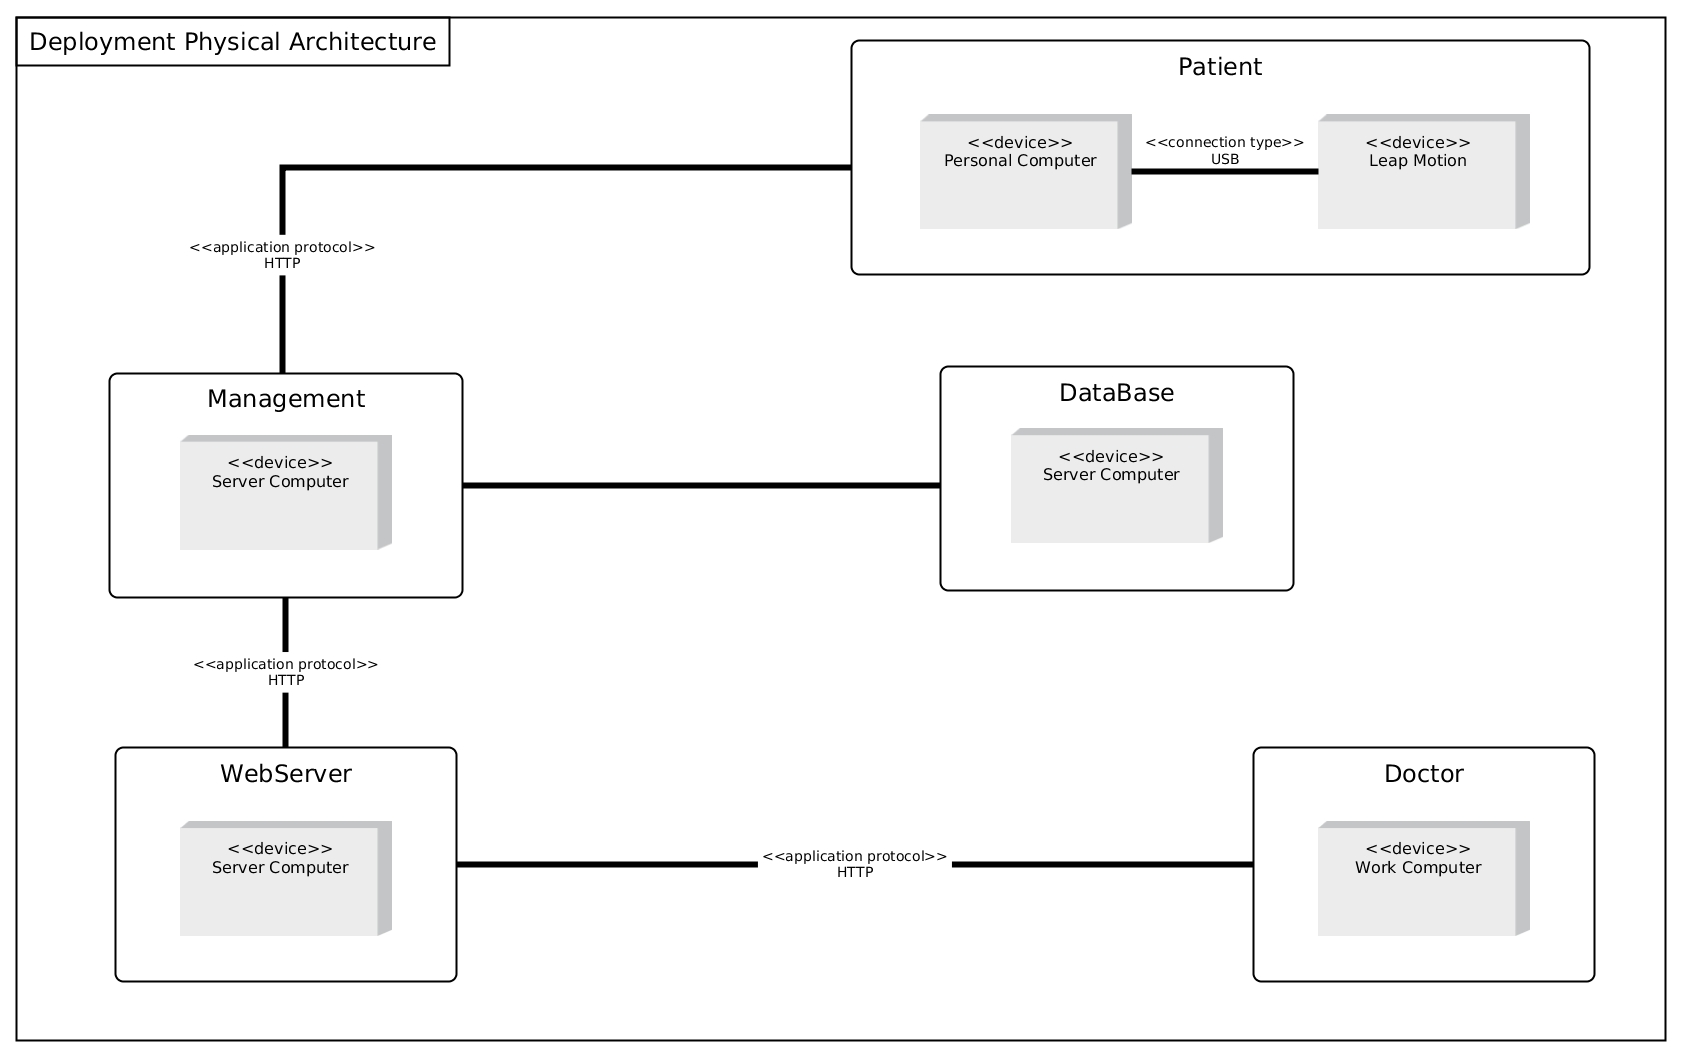
\includegraphics[scale=0.15]{./img/deployment.jpg}
    \caption{Diagrama de instalação.}
    \label{fig:deployment}
\end{figure}

A aplicação do paciente foi desenvolvida utilizando a framework electron para permitir a disponibilidade da aplicação em vários sistemas operativos sem ser necessário
alterar o código.
Os jogos foram desenvolvidos em JavaScript com recurso à biblioteca p5.js ou ao game engine Godot.

A aplicação do médico é uma webapp e foi desenvolvida utilizando HTML/CSS e JavaScript com recurso ao Django, uma framework para python.

A parte de gestão foi concebida através do Django e python para a REST API e MySQL para a base de dados (figura \ref{fig:tech_diagram}).

\begin{figure}[h!]
    \center
    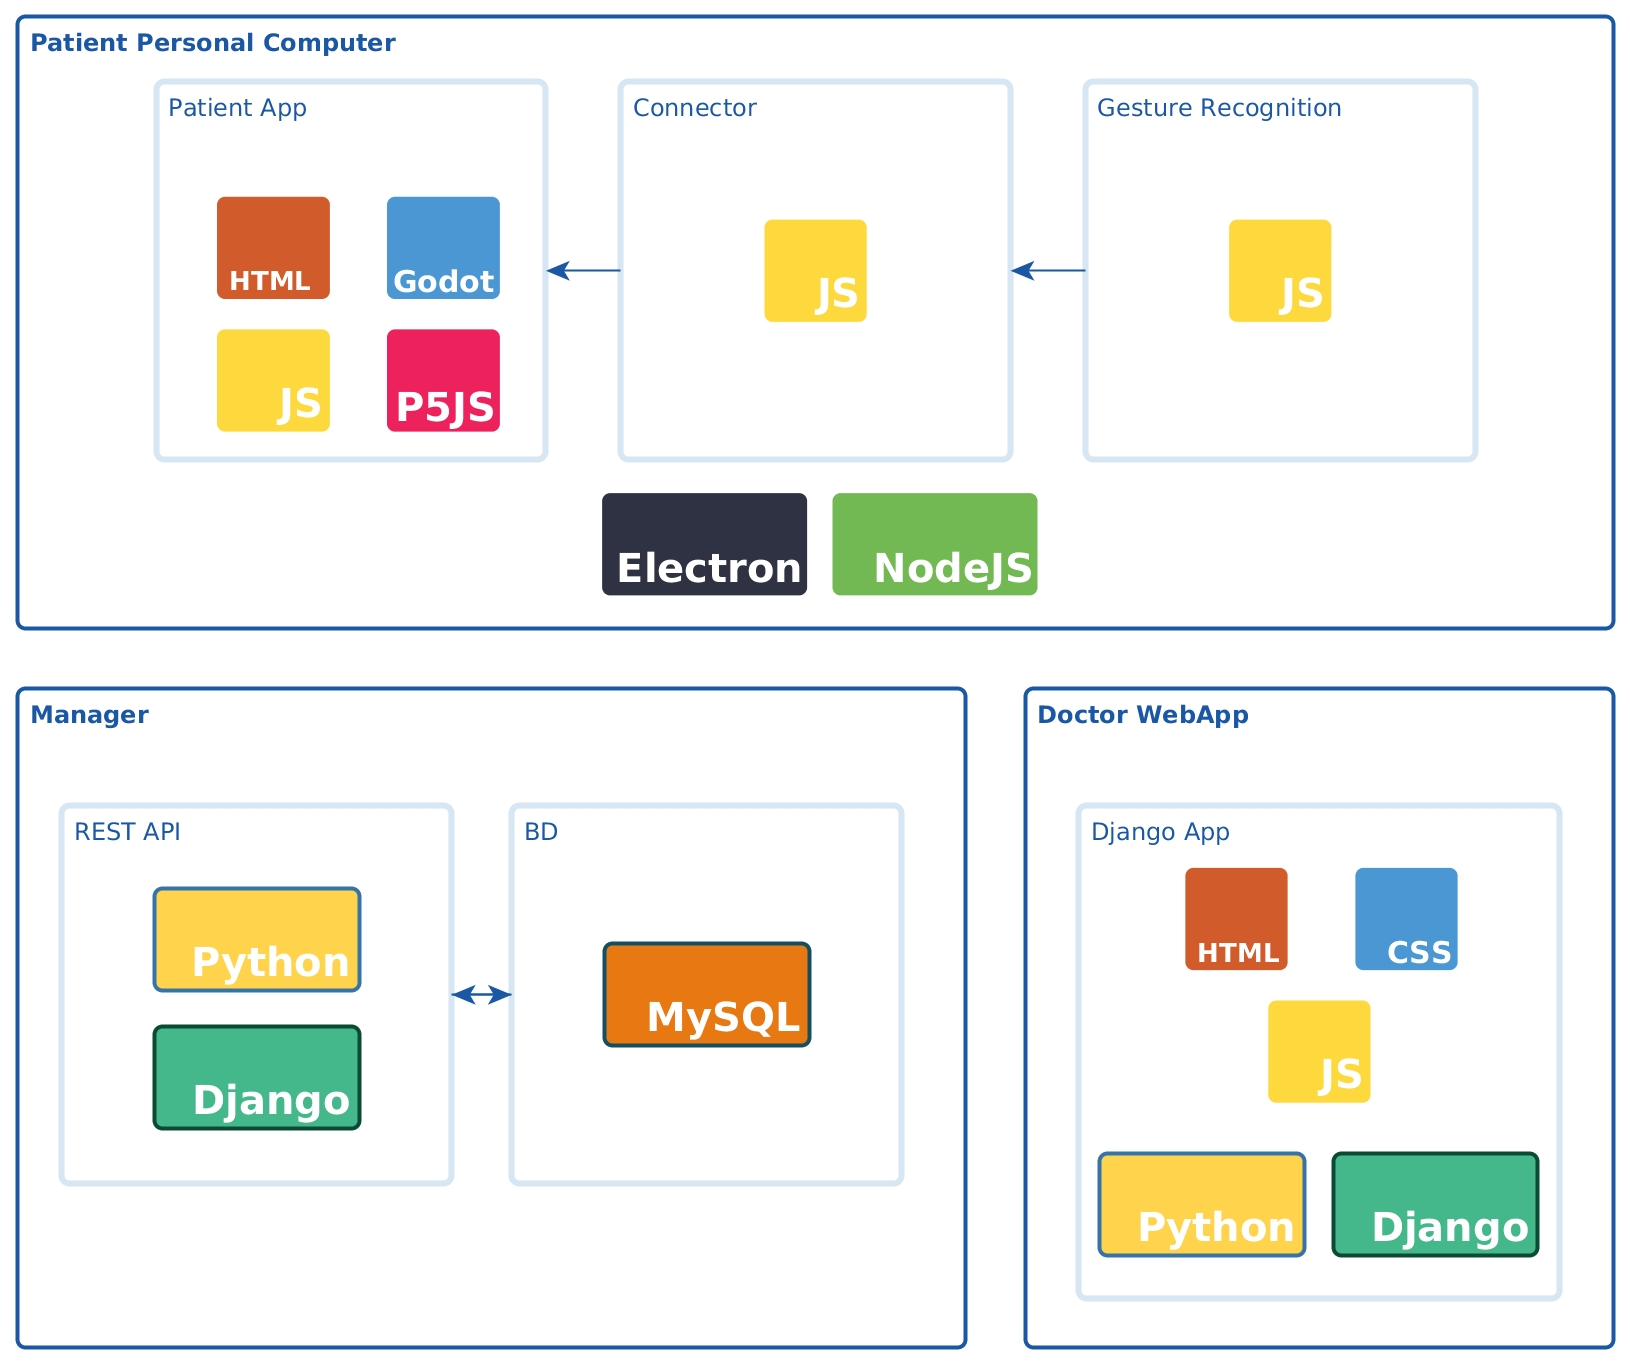
\includegraphics[scale=0.15]{./img/technological.jpg}
    \caption{Diagrama de tecnologias.}
    \label{fig:tech_diagram}
\end{figure}

No diagrama do modelo de domínio é possível evidenciar as várias relações existentes entre as diferentes entidades (figura \ref{fig:model_diagram}).
Este diagrama permitiu-nos programar mais facilmente as relações entre as várias entidades do sistema.

\begin{figure}[h!]
    \center
    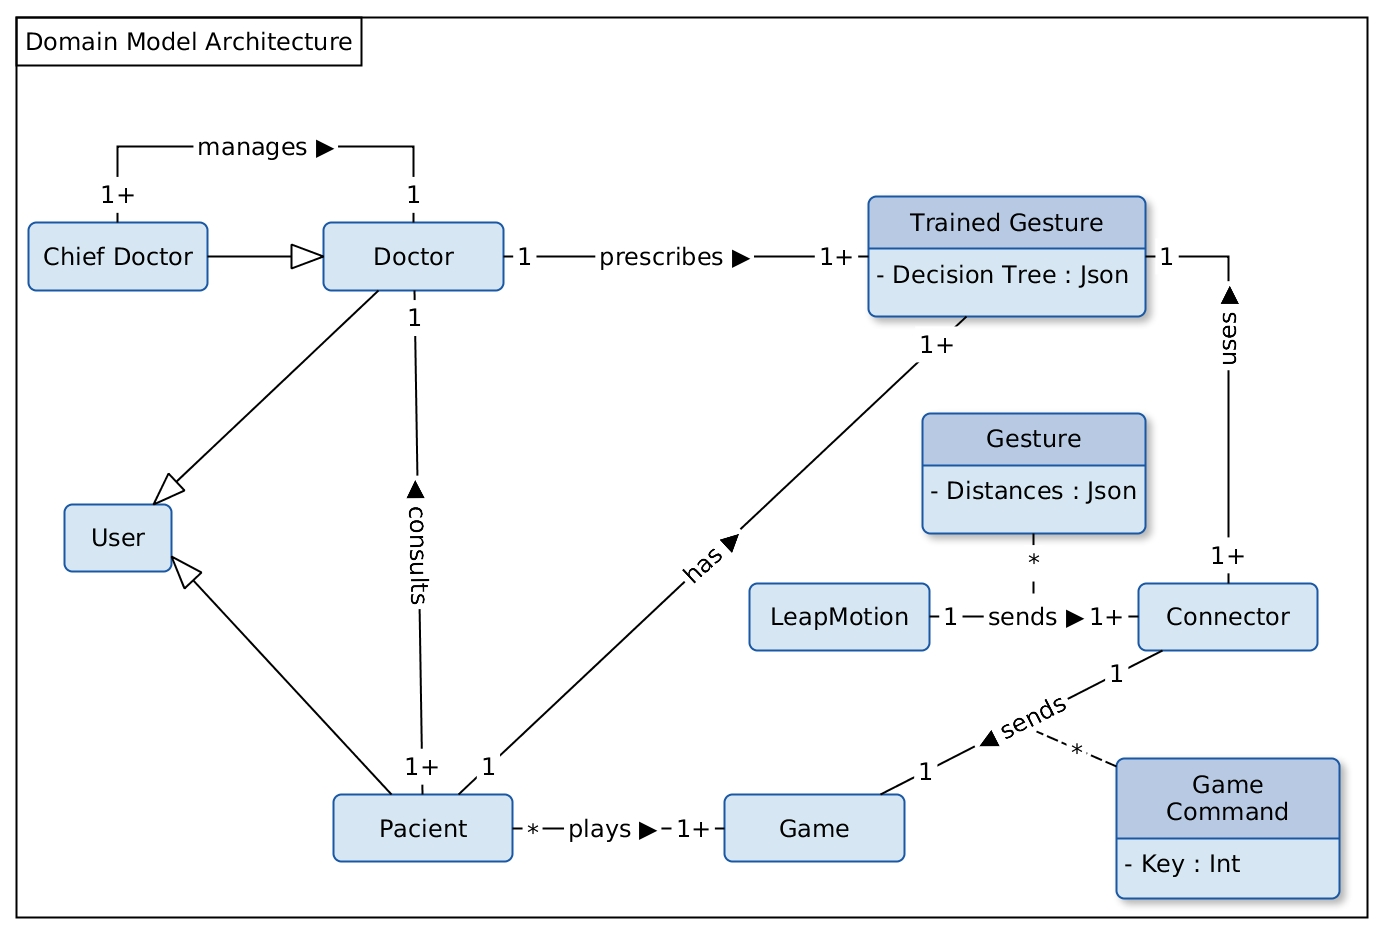
\includegraphics[scale=0.15]{./img/model.jpg}
    \caption{Diagrama do modelo de domínio.}
    \label{fig:model_diagram}
\end{figure}

\newpage

\subsection{Reconhecimento de Gestos}

Para implementar o reconhecimento com recurso a árvores de decisão foi utilizado a seguinte biblioteca: \url{https://github.com/lagodiuk/decision-tree-js},
que permite criar árvores de decisão e foram realizadas algumas alterações à mesma para permitir a serialização da árvore em formato json.

Por exemplo, o json:
\begin{verbatim}
{
"root":
  {
     "attribute":"n_extended_fingers",
     "predicate": [window.Function,[b,c],return b>=c],
     "predicateName":">=","pivot":4,"match":{"category":1},
     "notMatch":{"category":0}, "matchedCount":391,
     "notMatchedCount":412
  },
  "gesture_name":"open_hand"
}
\end{verbatim}

Representa a árvore de decisão para o gesto da mão aberta.

\subsection{Base de Dados}

A Base de Dados que está a ser utilizada para guardar toda a informação crucial ao funcionamento da nossa plataforma foi implementada em MySQL. O hosting da mesma foi feito com recurso ao serviço RDS (Amazon Relational Database Service).

Na figura \ref{fig:bd_diagram}, podemos encontrar o diagrama representativo da modelo lógico relacional de acordo com qual está formulada a Bases de Dados.

\begin{figure}[h!]
    \center
    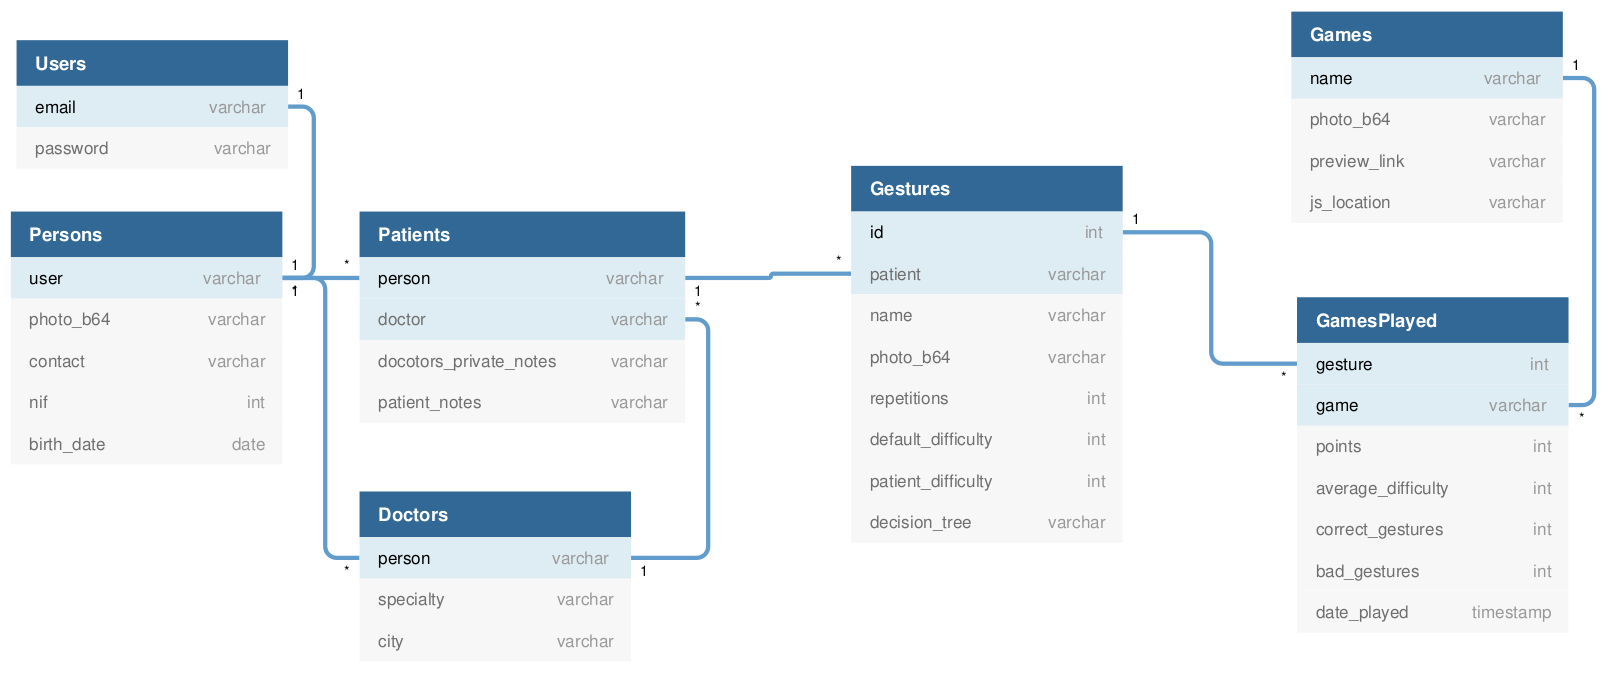
\includegraphics[scale=0.3]{./img/bd_diagram.png}
    \caption{Modelo lógico relacional da base de dados.}
    \label{fig:bd_diagram}
\end{figure}

\subsection{REST API}

Relativamente à REST API, esta foi construída com recurso ao framework Django, mais especificamente ao Django Rest Framework. Esta permite-nos uma enorme flexibilidade e agilidade, uma vez que é capaz de executar um rápido processamento de requests e facilmente lhe adicionamos novos métodos, que permitem executar novas operações.

\begin{itemize}
    \item \textbf{Django Models}: Utilizámos Django Models para criar entidades na base de dados, através de ORM (Object Relational Mapping).
    \item \textbf{Django Authentication}: Através de mecanismos de autenticação na API, conseguimos reconhecer qual o utilizador que se encontra a aceder à mesma.
    \item \textbf{Django Authorization}: Após um utilizador se autenticar, este apenas terá acesso a determinados recursos determinados pelo grupo em que este se insere.
    \item \textbf{Django REST Framework}: Permitiu a criação de uma REST API.
    \item \textbf{Django Core Mail}: Uma vez que os utilizadores são registados na plataforma pelo seu médico, estes irão receber, no seu e-mail, uma password que permitirá acesso à plataforma. Posteriormente, os pacientes poderão alterar a sua password.
\end{itemize}

\subsubsection{\textit{Queries}, Django ORM e Base de Dados}

Através dos recursos providenciados pelo Django, podemos muito facilmente manipular objetos da Base de Dados que está a ser utilizada pela API. O Django ORM permite-nos mapear entidades da base de dados em objetos de python, que podem, posteriormente, ser manipulados. É possível estabelecer relações entre entidades, bem como criar, remover ou editar qualquer entidade da base de dados.

Optámos por separar a lógica de acesso à base de dados, colocando-a, exclusivamente no ficheiro queries.py. Este tem todos as queries que estamos a executar.

\begin{figure}[h!]
    \center
    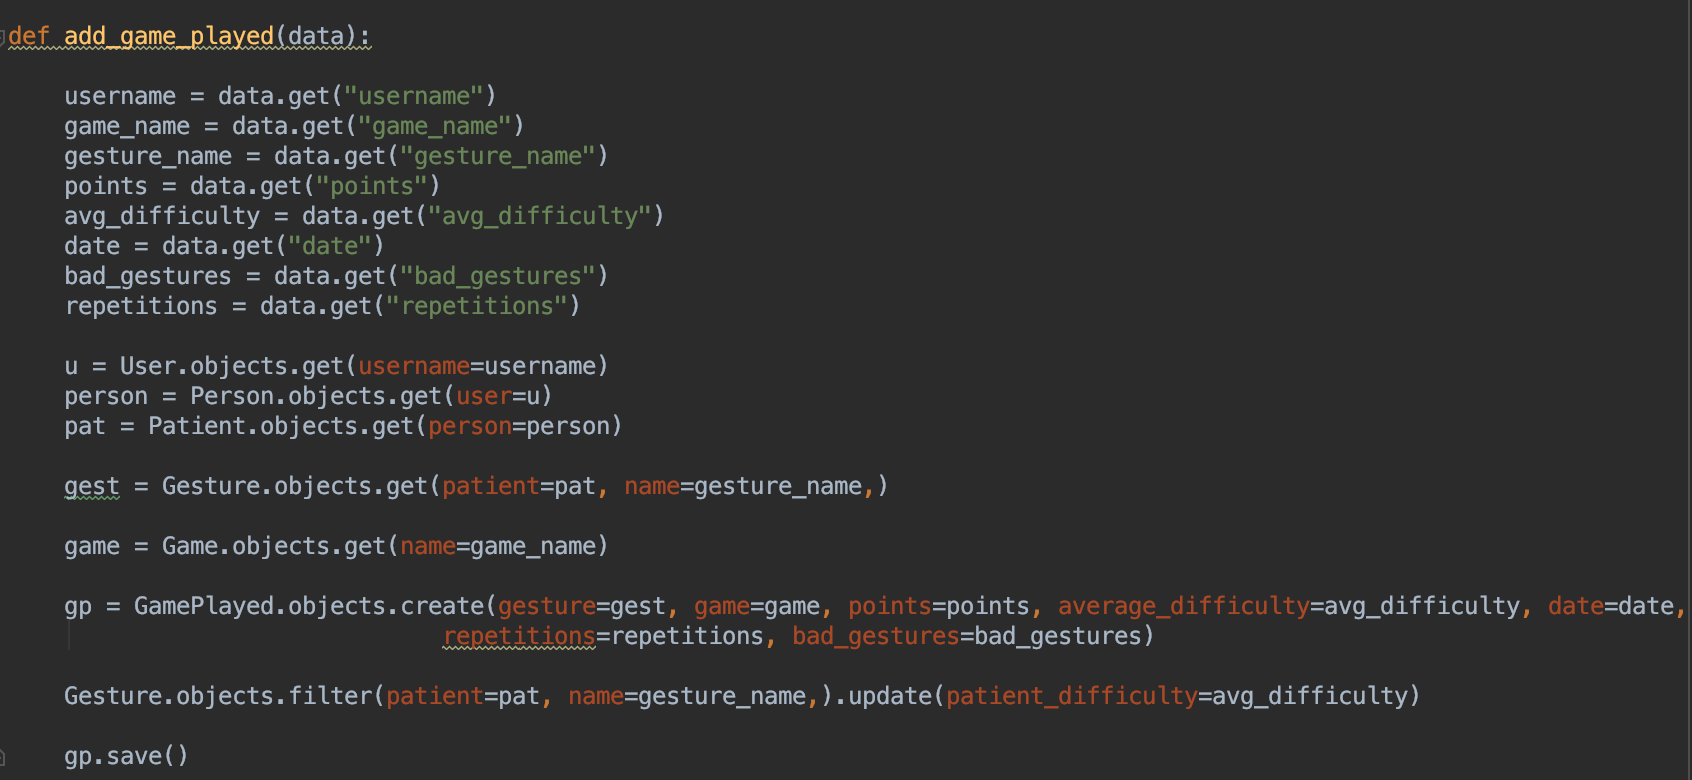
\includegraphics[scale=0.4]{./img/rest1.png}
    \caption{Excerto de código para adicionar informação sobre uma partida de um jogo.}
    \label{fig:rest1}
\end{figure}

É, desde já, importante referir que a Base de Dados se encontra completamente desacoplada da REST API que construímos, o que nos permite ter um sistema mais modular e reutilizável.

\begin{figure}[h!]
    \center
    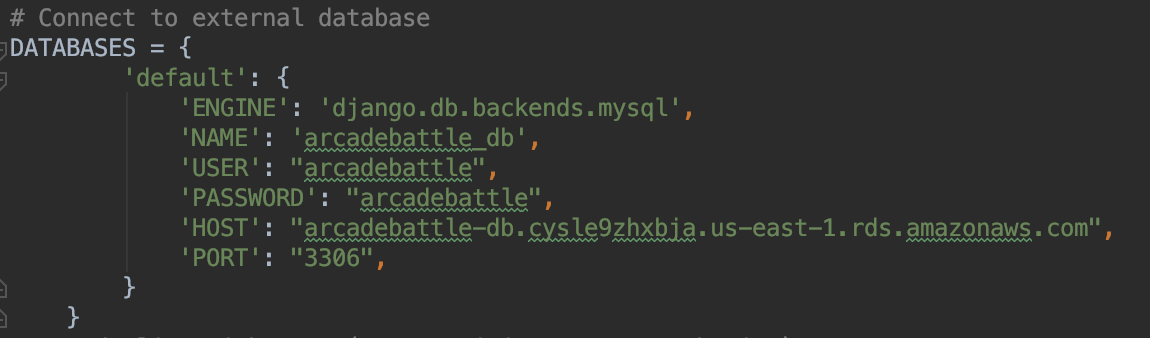
\includegraphics[scale=0.58]{./img/rest2.png}
    \caption{Excerto de código para configurar a comunicação com a base de dados.}
    \label{fig:rest2}
\end{figure}

\subsubsection{Autenticação e Autorização}
\label{sec:auth}

Uma vez que estamos a utilizar uma API REST para aceder à informação, os mecanismos de autenticação e autorização têm de existir ao nível desta API e não nas diferentes interfaces de acesso. Caso assim não fosse, seria possível obter informação crítica dos utilizadores da plataforma sem se estar autenticado no sistema.

Desta forma, optámos pela utilização de Auth Tokens, que devem acompanhar todos os pedidos feitos à REST API (excepto o pedido de log in).

Inicialmente, os utilizadores enviam os seus dados de autenticação através de um método POST, que, caso a autenticação seja bem sucedida, retorna ao utilizador um Auth Token que este deve guardar para posteriores pedidos. Este Auth Token é, também, guardado pelo sistema, de forma a verificar se um utilizador pode, ou não, aceder ao mesmo.

\begin{figure}[h!]
    \center
    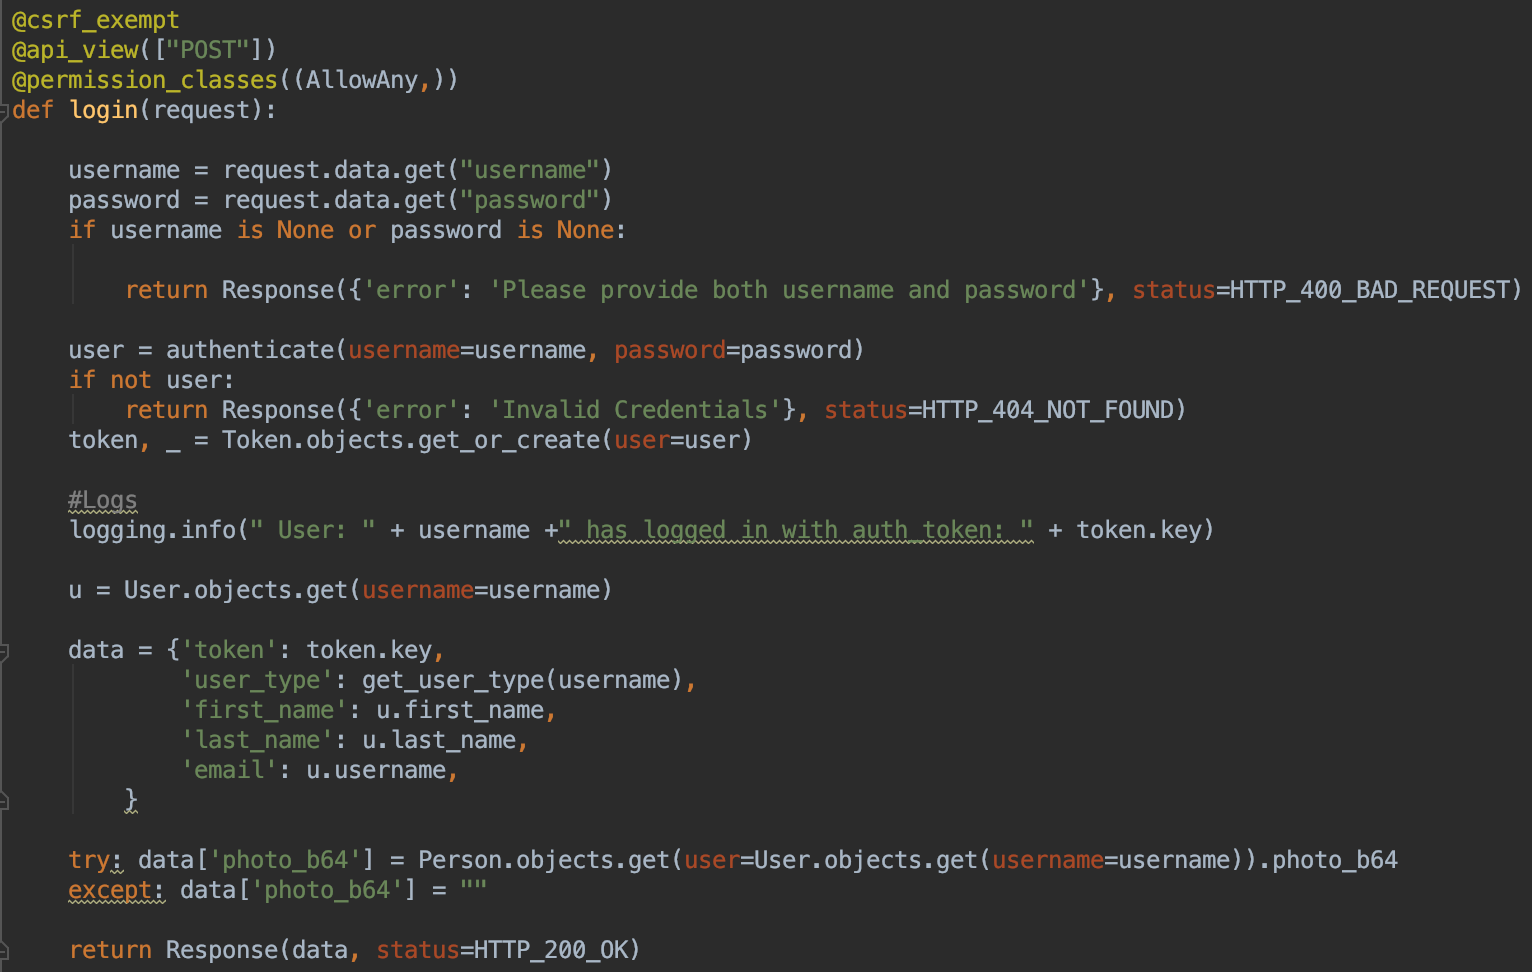
\includegraphics[scale=0.43]{./img/rest3.png}
    \caption{Excerto de código para realizar a autenticação no sistema.}
    \label{fig:rest3}
\end{figure}

Quando acaba o tempo de vida do Auth Token ou o paciente sai da plataforma (logout), este Auth Token é removido do sistema, sendo que, num futuro acesso do mesmo utilizador, um novo Token será gerado.

É, novamente, na API que é verificada a autorização que um utilizador detém para aceder a determinados recursos. Por exemplo, um paciente, não poderá remover um médico.
Assim sendo, a API, utiliza o grupo e o tipo de entidade associado a cada utilizador, de forma a determinar se este pode aceder à informação que está a requisitar.

Para uma autenticação segura e mais cómoda criamos também a possibilidade de autenticação com o cartão de cidadão português.
Para realizar o processo de autenticação de um modo seguro é utilizado uma estratégia do tipo desafio-resposta (ver figura \ref{fig:auth_diagram}).

O cliente começa por fazer um pedido ao servidor para indicar a sua intenção de se autenticar, junto com este pedido envia o certificado de autenticação
do cartão de cidadão. Do lado do servidor é feita a validação do certificado e é criada uma associação entre o certificado e um timestamp (do momento atual),
de seguida o servidor responde com o timestamp (desafio), o cliente irá utilizar o certificado de autenticação para assinar o timestamp (resposta)
e vai enviá-la para o servidor, e este vai verificar a validade a mesma. Se esta estiver correta envia para o cliente um cookie referente à sessão, caso contrário envia
uma mensagem de erro.

\begin{figure}[h!]
    \center
    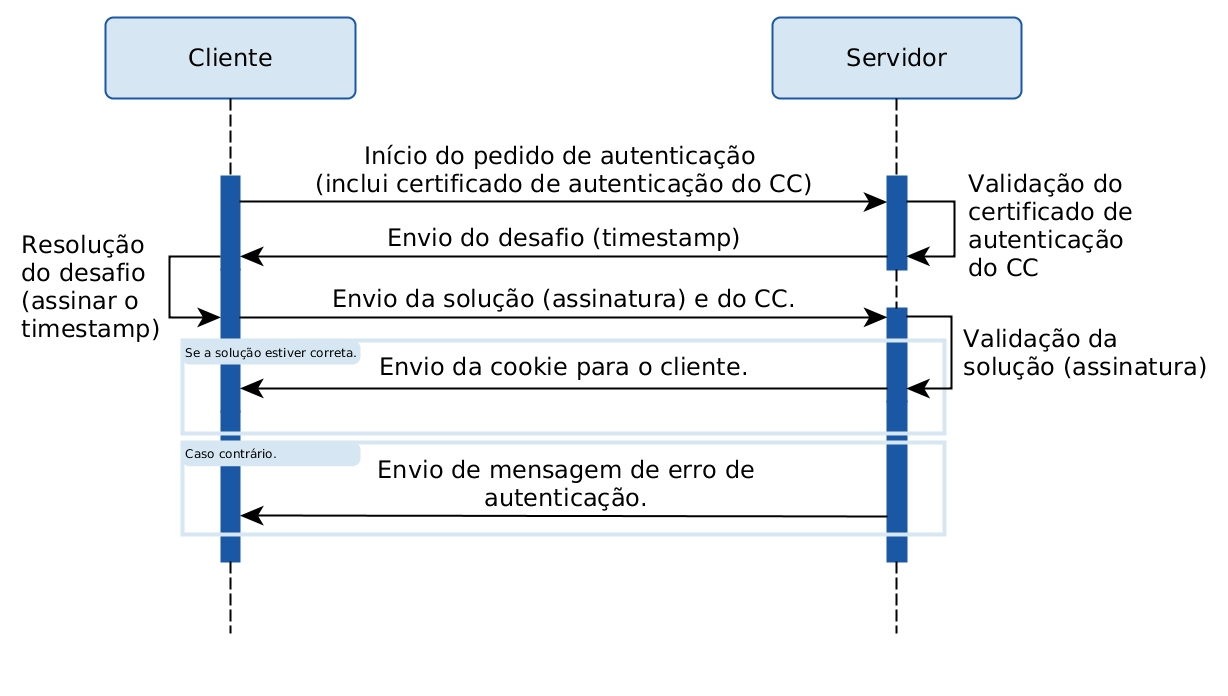
\includegraphics[scale=0.3]{./img/authentication.jpg}
    \caption{Diagrama de sequência do processo de autenticação com o cartão de cidadão de cidadão.}
    \label{fig:auth_diagram}
\end{figure}

\subsubsection{Envio Automático de E-mails}

Recorrendo ao Django Core e-mail a nossa plataforma é capaz de enviar automaticamente e-mails aos mais diversos utilizadores.

A introdução desta funcionalidade, prende-se com o facto de ser o médico a registar os novos pacientes na plataforma. Esta envia automaticamente um e-mail para o paciente com os seus dados de acesso, que posteriormente podem ser alterados.

Para que isto seja possível, é necessário criar um endereço de e-mail (aquele que será associado à plataforma), conhecer qual o DNS do servidor SMTP a este associado e configurar tudo isto no ficheiro settings.py da API.

\begin{figure}[h!]
    \center
    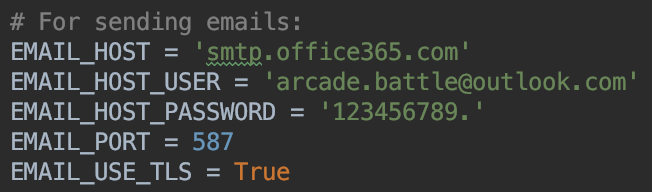
\includegraphics[scale=0.65]{./img/rest4.png}
    \caption{Excerto de código para configurar as variáveis referentes ao email.}
    \label{fig:rest4}
\end{figure}

Podemos ter alguns problemas dentro de determinadas redes, como por exemplo, dentro da rede da Universidade de Aveiro, que não se consegue conectar ao servidor SMTP, embora tal seja perfeitamente exequível dentro das redes domésticas onde testámos o sistema.

\subsection{Plataforma do Médico}

O médico, enquanto ator no sistema, tem a possibilidade de adicionar/remover pacientes à plataforma, escrever notas partilhadas ou privadas do paciente,
observar as estatísticas dos mesmos e, principalmente, numa fase de consulta, ajudar o paciente a adicionar os gestos ao sistema para que este possa mais
tarde enfrentar o processo de reabilitação que irá consistir em jogar os jogos disponíveis na plataforma usando os gestos adicionados na consulta.

Todos os componentes referentes ao médico foram desenvolvidos em Django seguindo uma arquitetura modular, mais especificamente, uma arquitetura de 3 camadas:
camada de apresentação, camada de lógica e camada de dados. Com isto, esta arquitetura apresenta vantagens como:

\begin{itemize}
    \item Todas as camadas são independentes o que implica que mudanças na plataforma afetem apenas a camada onde se está a trabalhar;
    \item Maior facilidade em termos de manutenção;
    \item Os diferentes componentes são reusáveis;
    \item Rapidez de desenvolvimento através da divisão de trabalho.
\end{itemize}

Para a interface do médico, cada url é mapeado através de uma view. Nestas views, são feitos essencialmente os pedidos à REST API onde se obtém conteúdo que se pretende mostrar na interface. Foi ainda construído o suporte para autenticação com cartão de cidadão. Neste tópico foram ainda utilizadas funcionalidades próprias do Django como:

\begin{itemize}
    \item Django Forms: Como forma de acesso estruturado aos dados e validação dos mesmos.
    \item Integração com a Leap Motion (\url{www.leapmotion.com}): O nosso sistema integra o  Leap Motion SDK, o que permite a recolha de um gesto realizado por um paciente, que será posteriormente guardado na Base de Dados.
\end{itemize}

\subsubsection{Adicionar/Remover Paciente}
O médico consegue, através de um formulário, adicionar facilmente um novo paciente à sua lista de pacientes.

\begin{figure}[h!]
    \center
    \frame{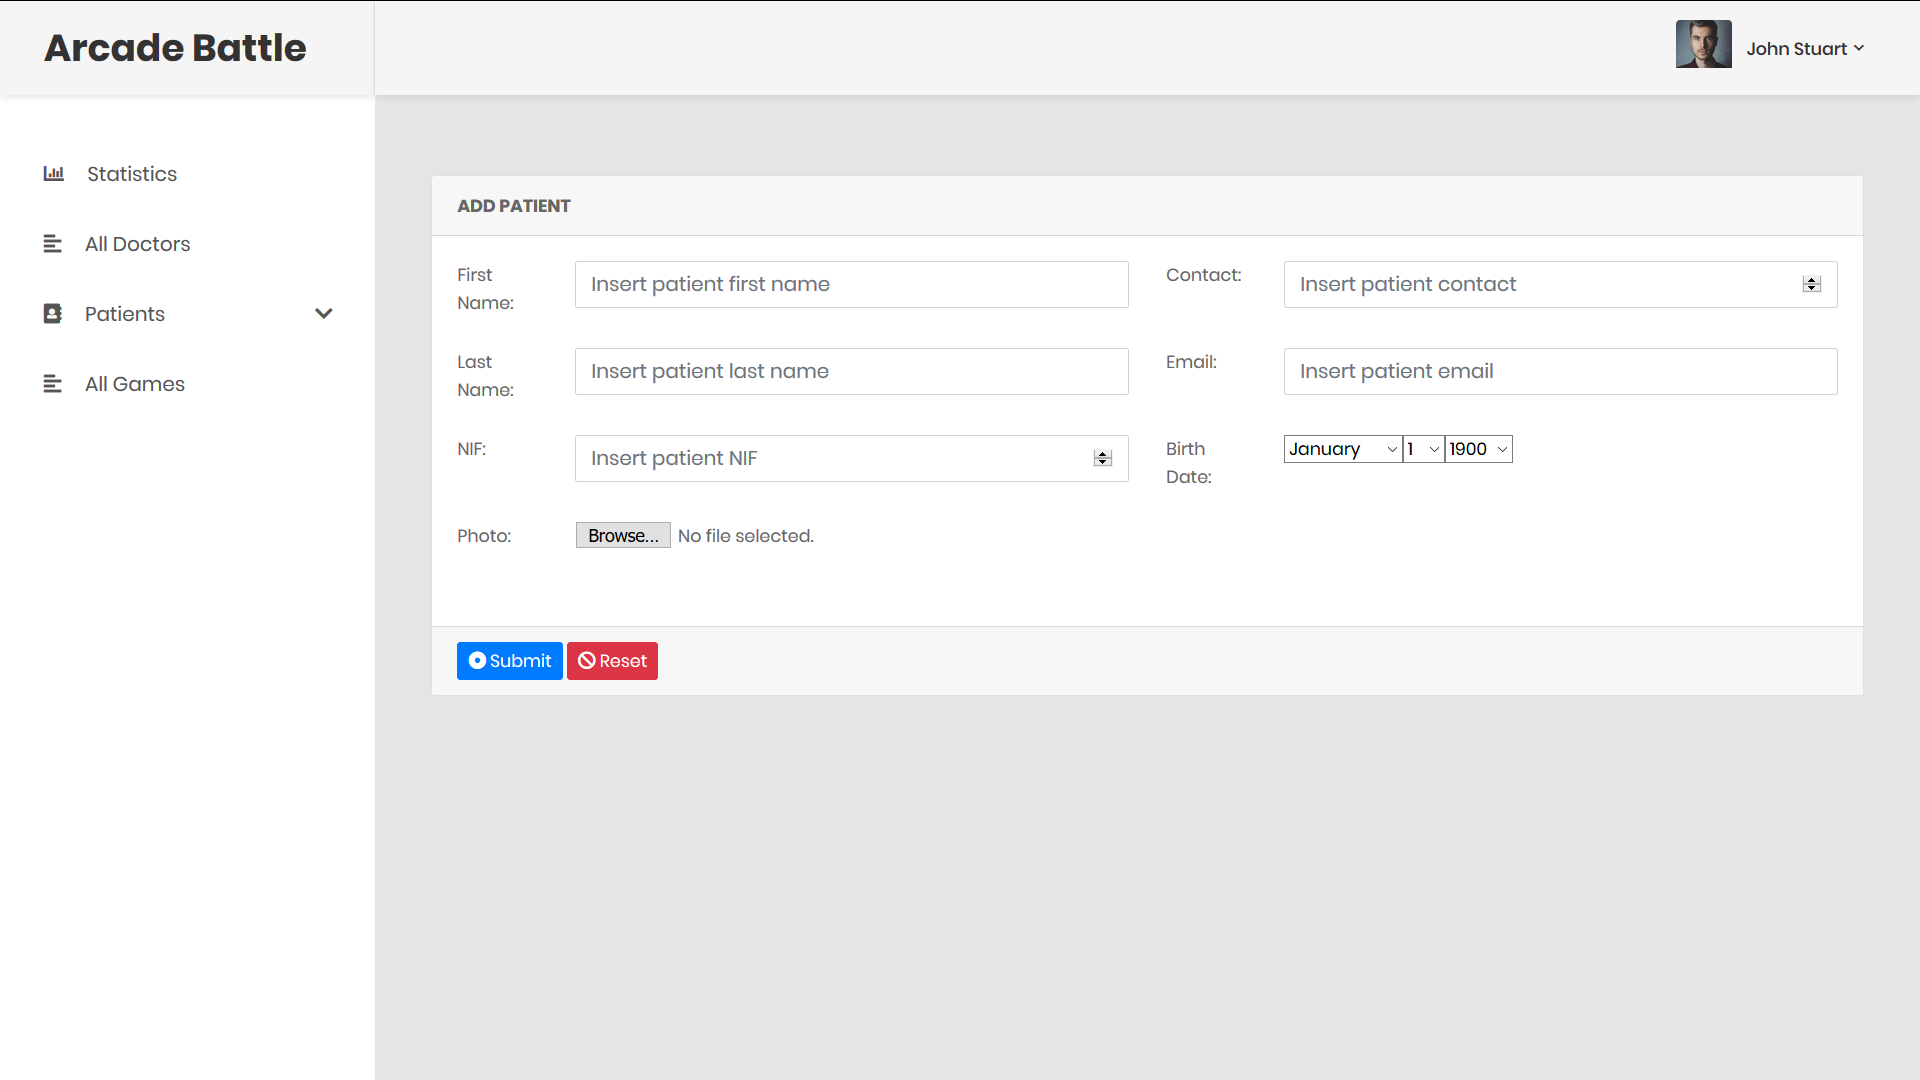
\includegraphics[scale=0.15]{./img/doctor1.png}}
    \caption{Página para adicionar/remover pacientes.}
    \label{fig:doctor1}
\end{figure}

Posteriormente, se o médico pretender remover algum paciente adicionado, pode sempre aceder à lista de pacientes e remover carregando no botão “Remove”.

\begin{figure}[h!]
    \center
    \frame{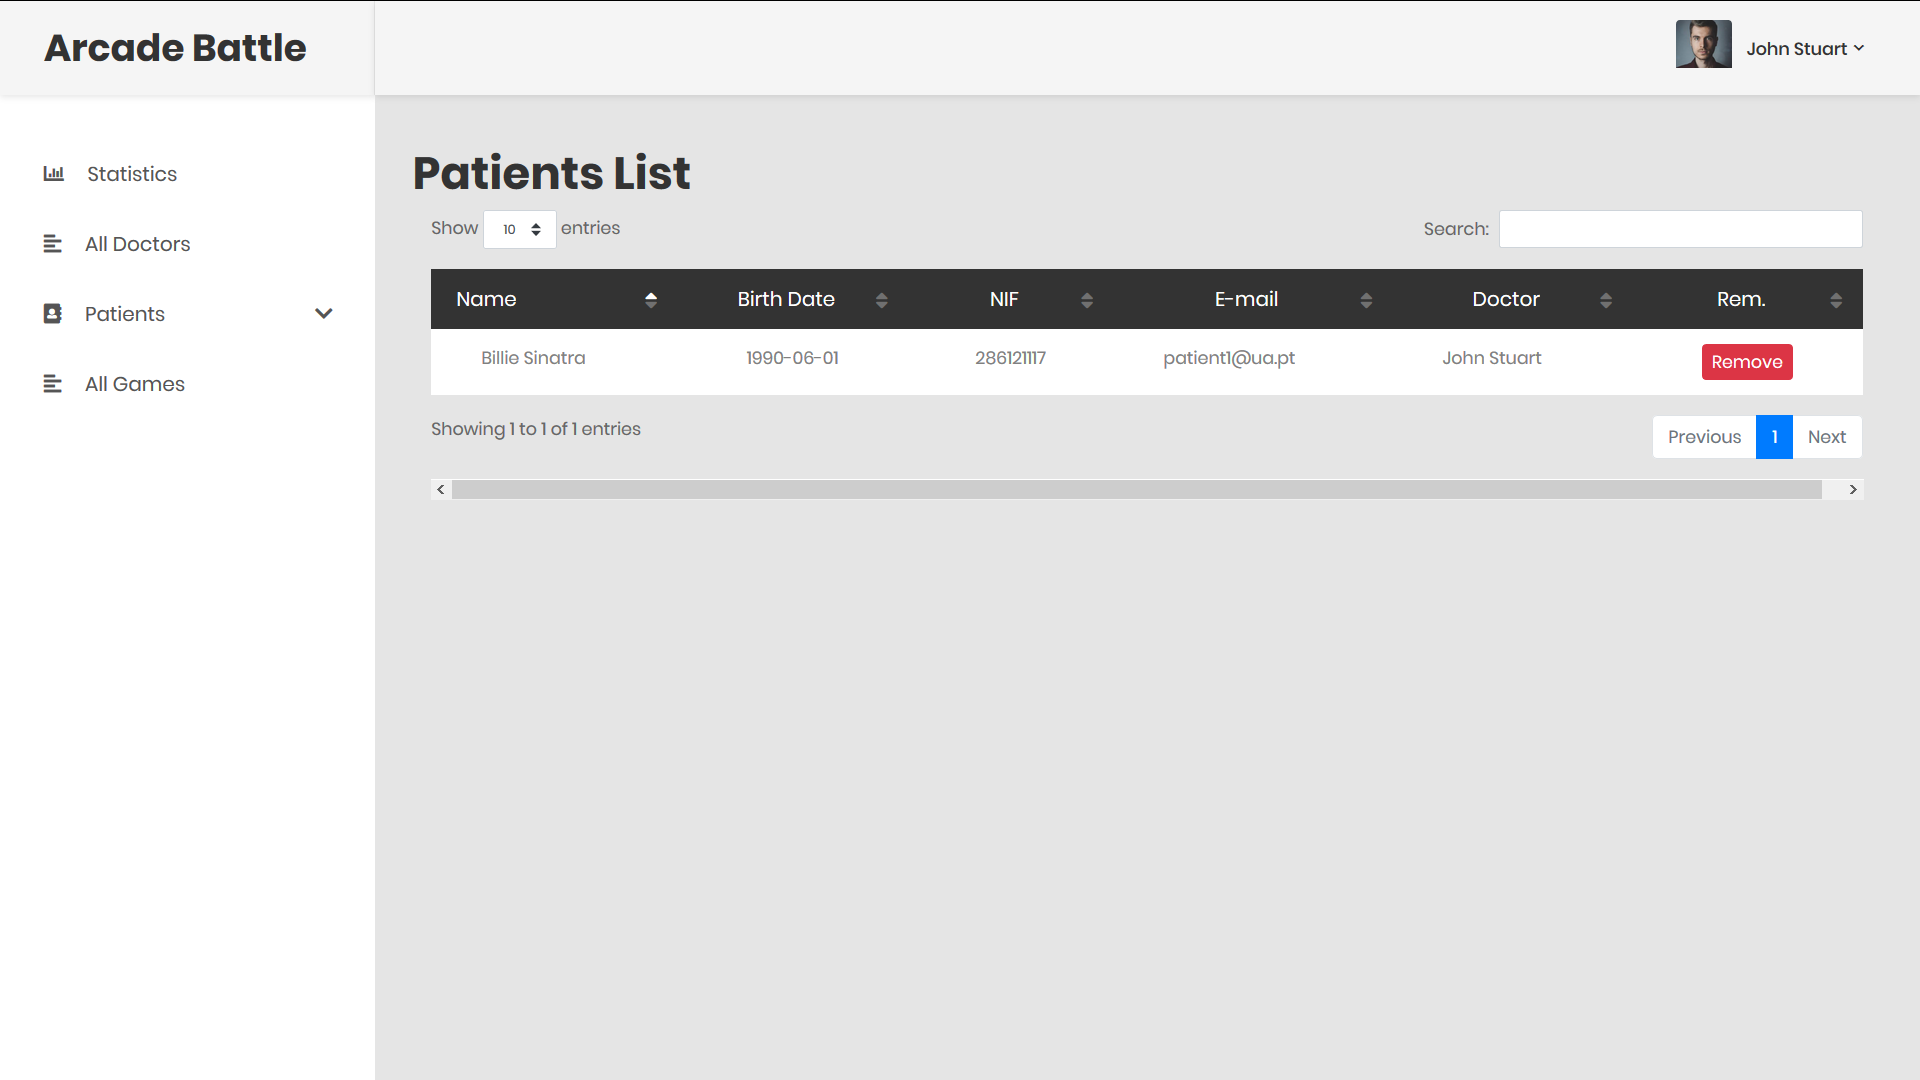
\includegraphics[scale=0.15]{./img/doctor2.png}}
    \caption{Página com a lista de pacientes.}
    \label{fig:doctor2}
\end{figure}

\newpage


\subsubsection{Adicionar Gestos}

Para que o paciente possa exercer a reabilitação indicada pelo médico, este pode numa consulta, através de um formulário,
adicionar um novo gesto para o paciente fazendo com que este seja treinado com a mão do paciente. Através deste formulário, o médico pode definir o número de repetições adequado para o paciente assim como a dificuldade inicial associada ao gesto. Esta dificuldade vai ser utilizada como método de comparação com a dificuldade que o paciente conseguir atingir no processo de reabilitação.

\begin{figure}[h!]
    \center
    \frame{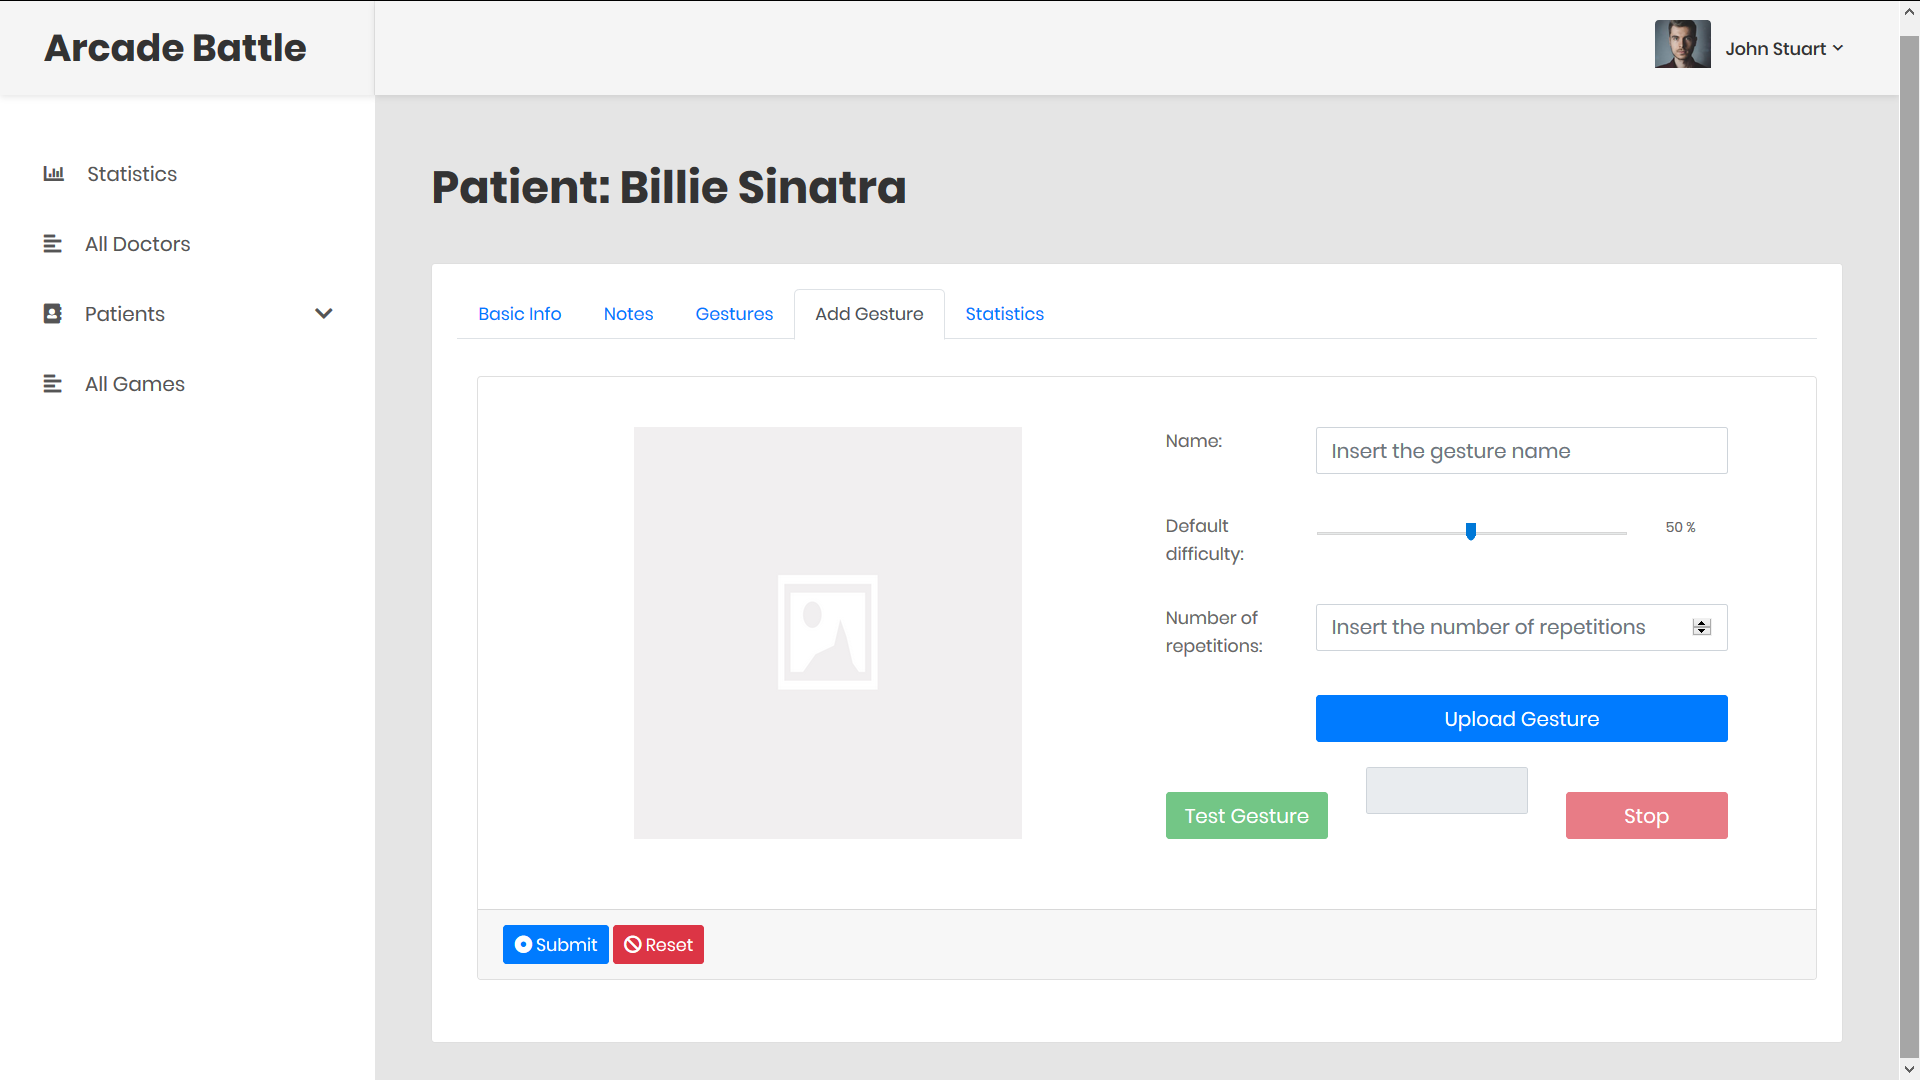
\includegraphics[scale=0.15]{./img/doctor5.png}}
    \caption{Página para adicionar um gesto.}
    \label{fig:doctor5}
\end{figure}
\newpage
\subsubsection{Observar estatísticas}

Dentro da informação de uma paciente, para além dos dados do paciente, o médico conseguirá aceder a estatísticas como:

\begin{itemize}
    \item Estatísticas gerais sobre gestos corretos/falhados, número de jogos jogados em relação a cada jogo e dificuldades associadas a cada gestos.
    \begin{figure}[h!]
        \center
        \frame{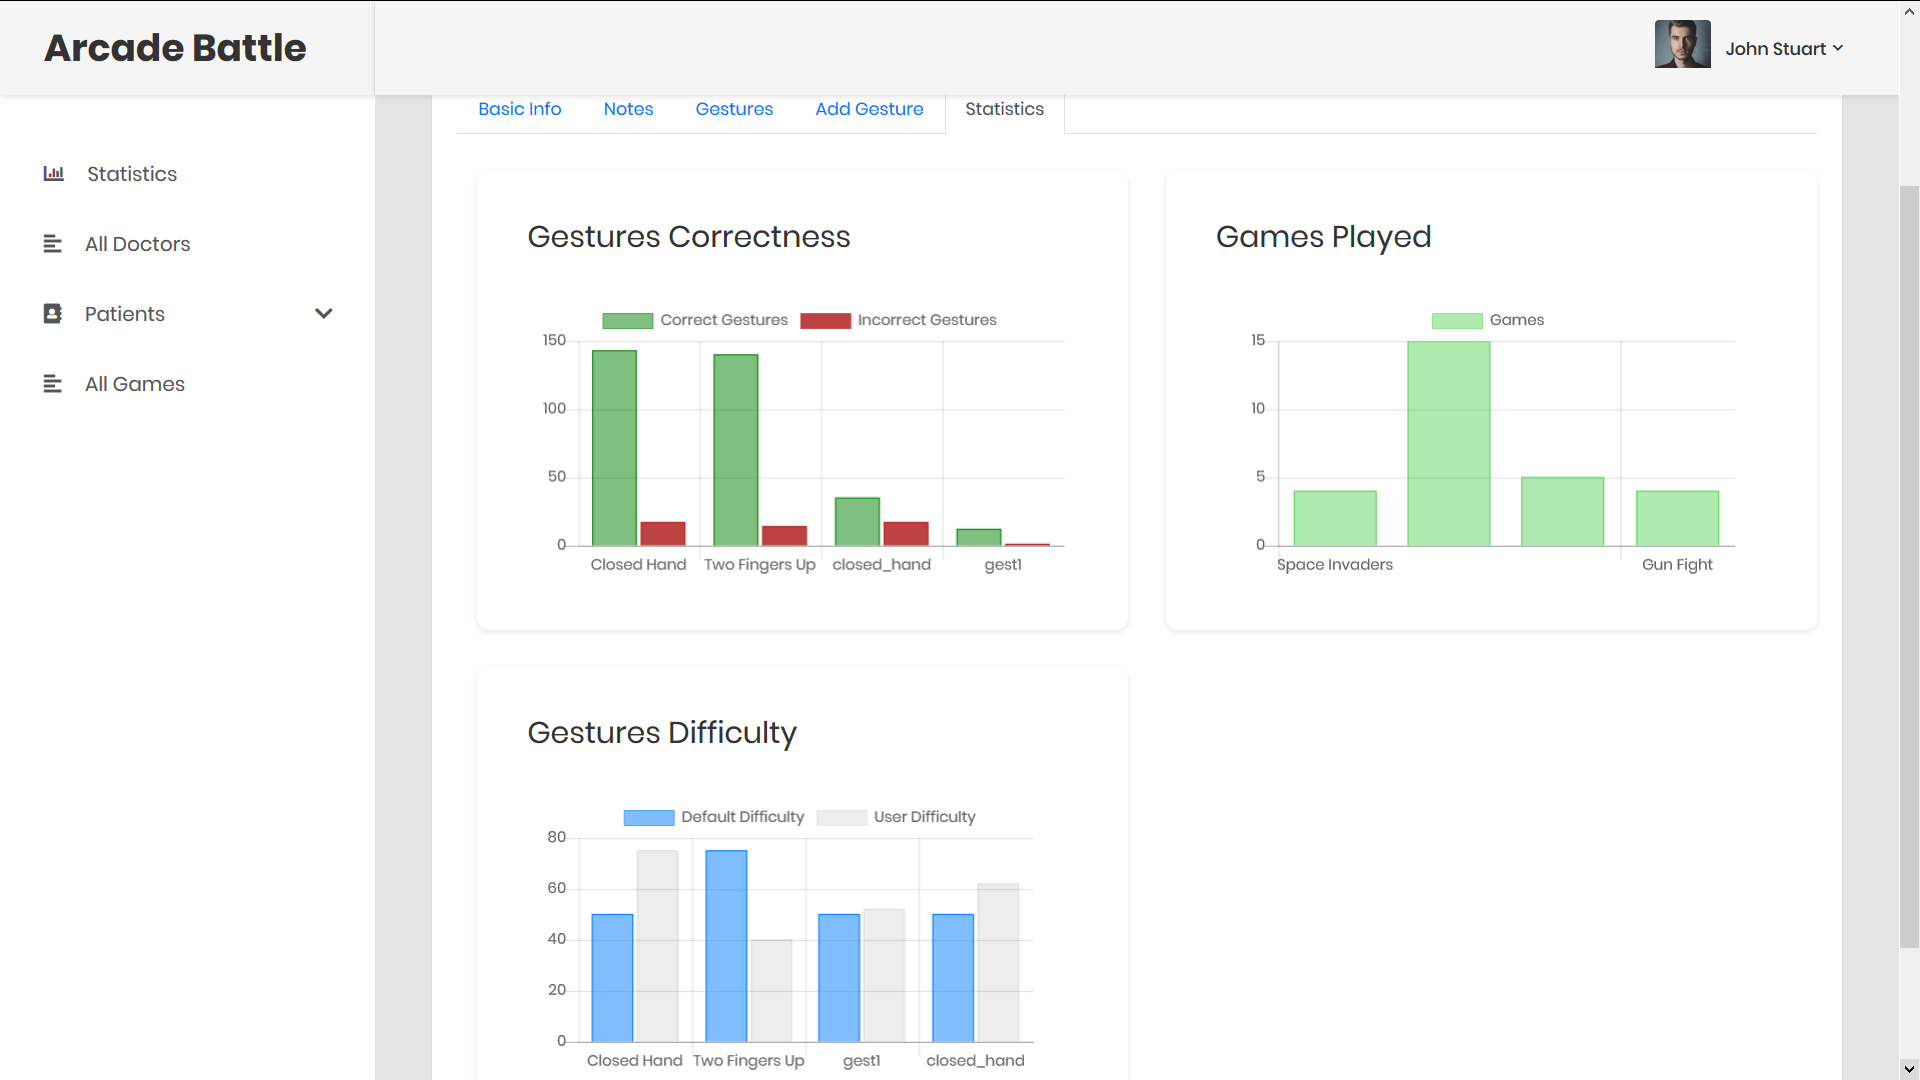
\includegraphics[scale=0.15]{./img/doctor4.png}}
        \caption{Página com estatísticas gerais.}
        \label{fig:doctor4}
    \end{figure}
    \item Estatísticas particulares sobre o gesto de um paciente que ajudam a demonstrar a evolução do paciente através do número de gestos corretos e
          de gestos falhados e da dificuldade atual do gesto.
    \begin{figure}[h!]
        \center
        \frame{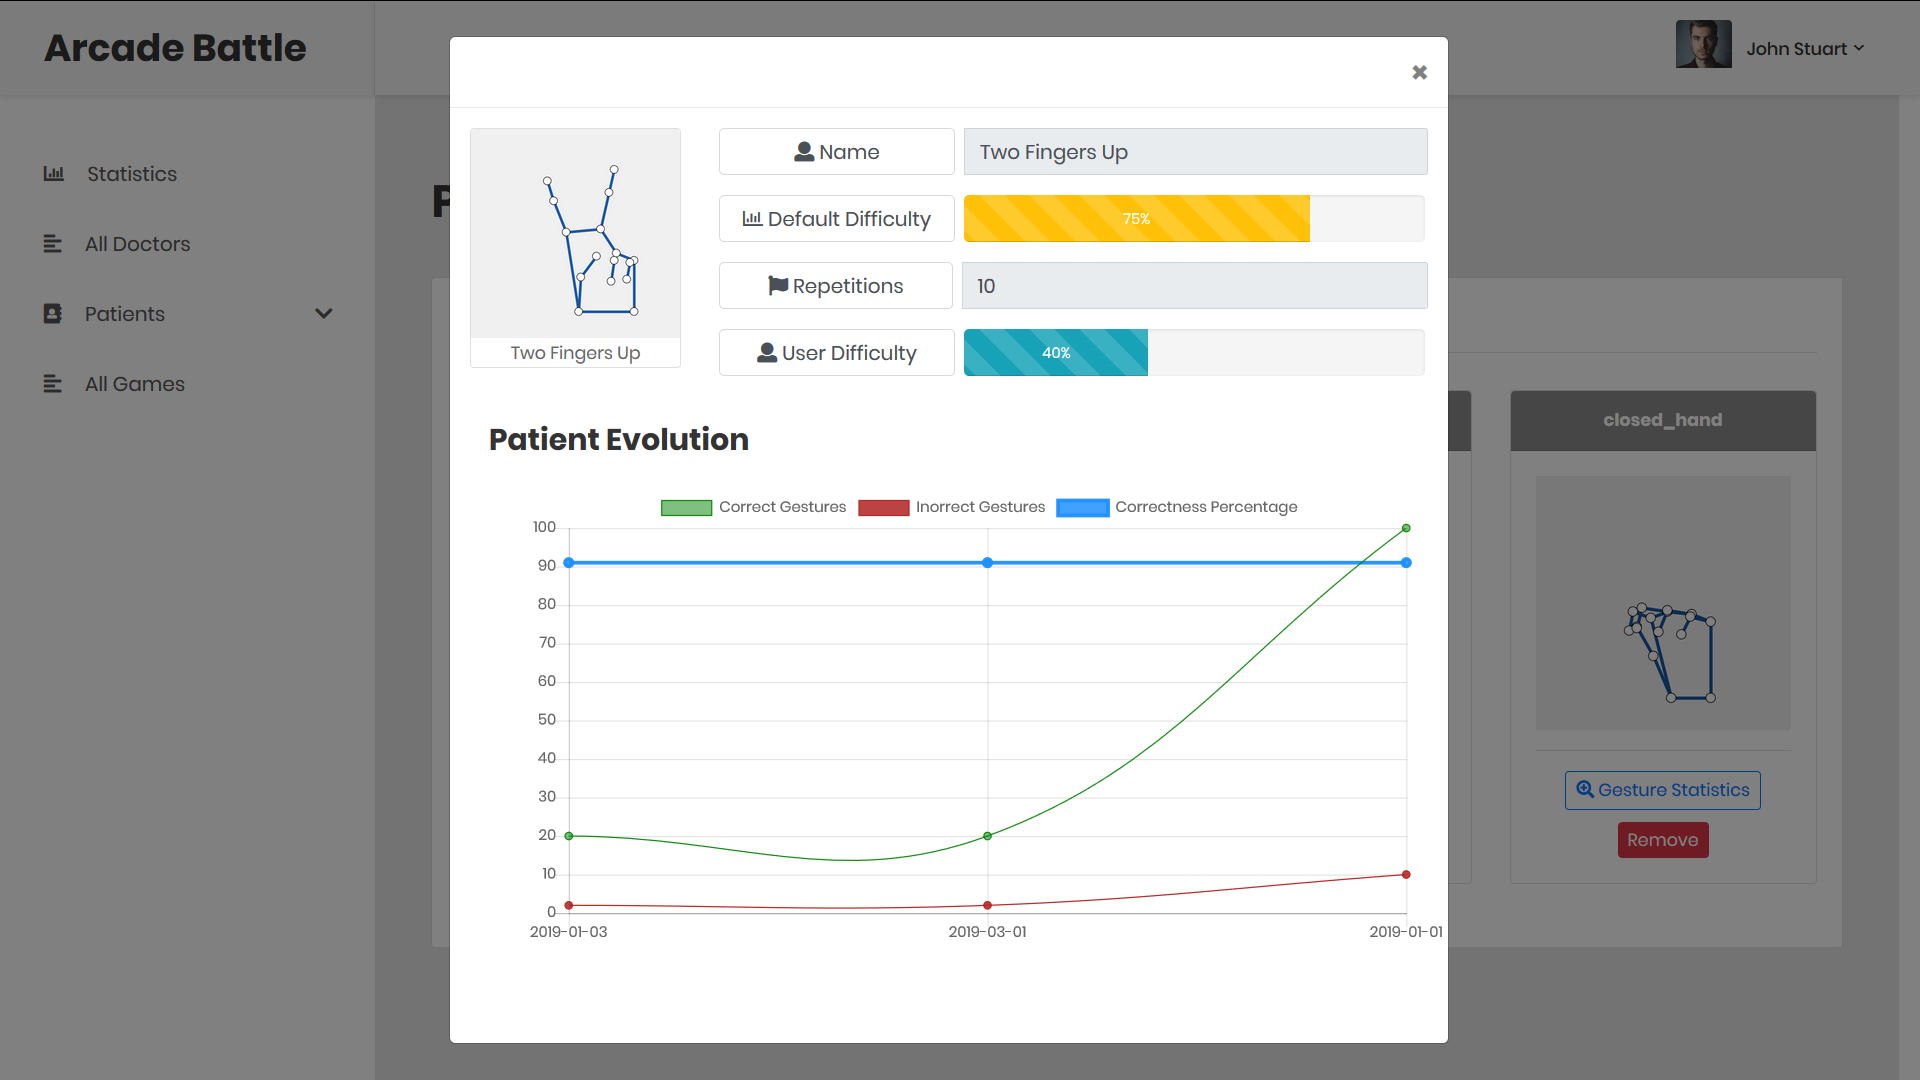
\includegraphics[scale=0.15]{./img/doctor3.png}}
        \caption{Página com estatísticas sobre um gesto.}
        \label{fig:doctor3}
    \end{figure}
\end{itemize}

\newpage

\subsubsection{Escrever Notas Privadas ou Partilhadas com o Paciente}

Após alguns testes de usabilidade feitos por médicos, concluímos que um médico pode escrever notas privadas sobre o paciente, ou seja,
notas a que o paciente não tenha acesso, e que pode escrever notas que serão partilhadas com o paciente.

\begin{figure}[h!]
    \center
    \frame{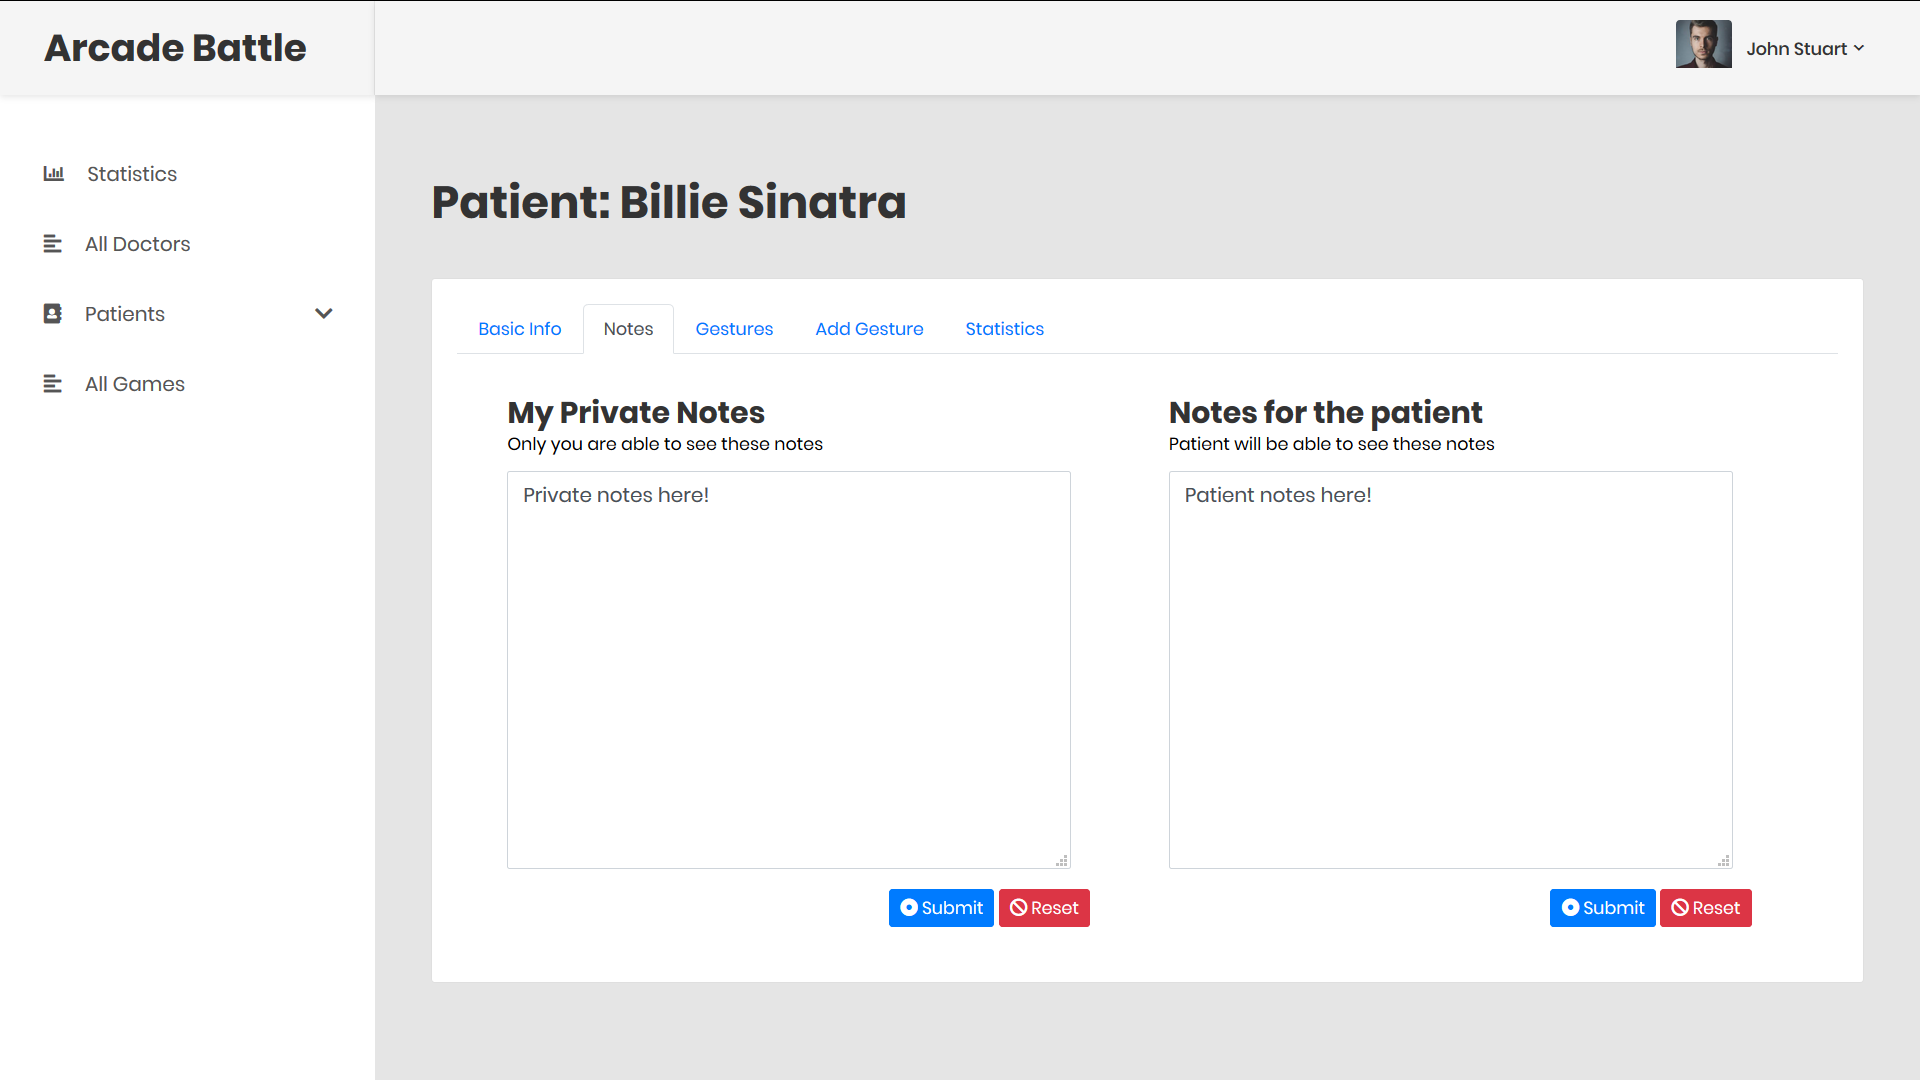
\includegraphics[scale=0.15]{./img/doctor6.png}}
    \caption{Página com as notas do médico.}
    \label{fig:doctor6}
\end{figure}

\subsection{Plataforma do Paciente}

Esta secção faz uma análise do trabalho desenvolvido na aplicação do paciente.

Analisaremos, também, os métodos de desenvolvimento dos vários módulos, bem como as razões que nos levaram à adoção dos métodos em causa.
Para além disto, explicaremos qual a origem e a motivação inerentes ao desenvolvimento de cada módulo.

Uma vez que o produto final é uma aplicação desenvolvida utilizando a framework electron, toda a aplicação do paciente foi desenvolvida como sendo uma aplicação web
que consome a REST API acima descrita para obter a informação necessária a representar.

O facto de esta aplicação utilizar a framework electron permite que esta possa ser multiplataforma e como tal, executada em vários sistemas operativos (Linux, macOS e Windows).

\subsubsection{Autenticação}

Como mencionado acima a interface do paciente consome os recursos da API disponibilizada, sendo que a autenticação é feita da forma referida em \ref{sec:auth}.
Isto exige, como referido no levantamento de requisitos, que o paciente tenha uma conexão à internet.

\begin{figure}[h!]
    \center
    \frame{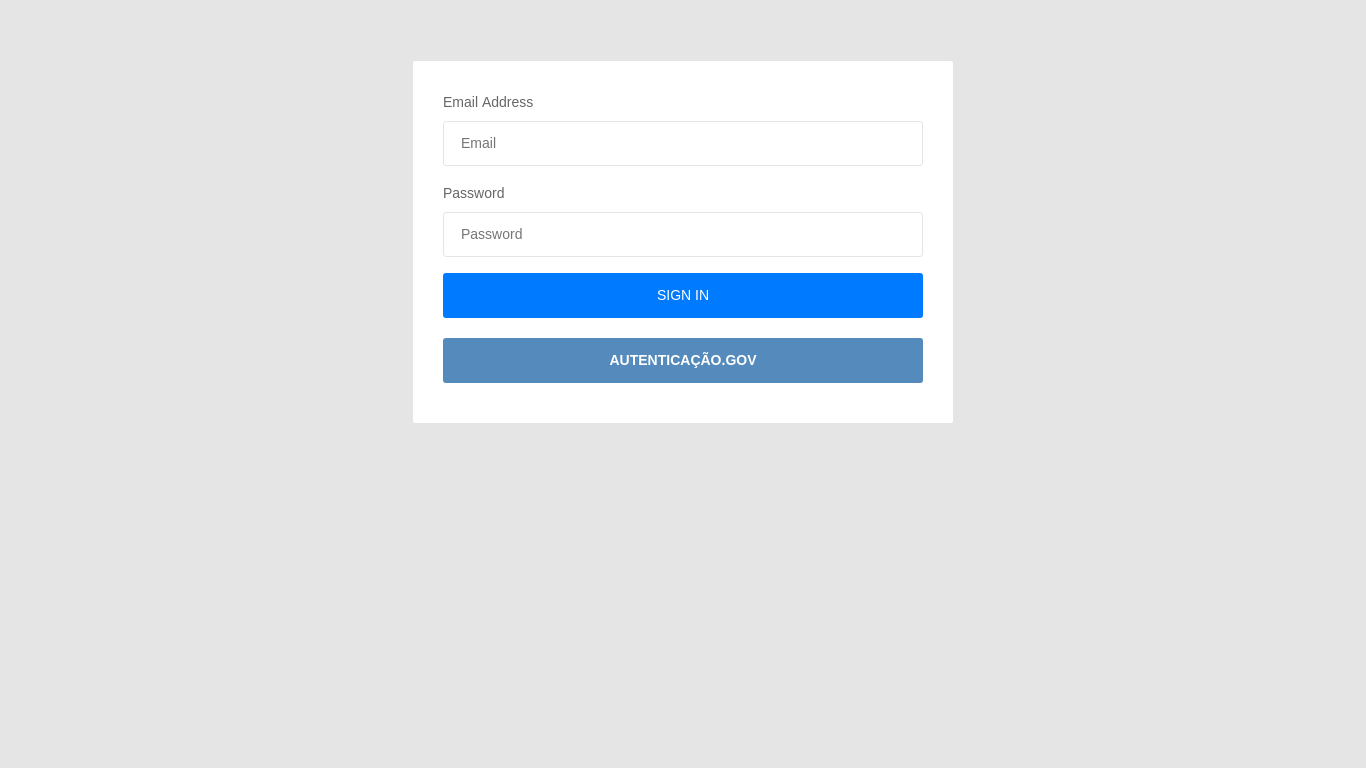
\includegraphics[scale=0.25]{./img/patient1.png}}
    \caption{Página de login.}
    \label{fig:patient1}
\end{figure}

Após a autenticação um token é guardado em local storage para os pedidos futuros.

\subsubsection{Jogos}

Após realizar a autenticação o paciente é redirecionado para a página dos jogos, onde pode visualizar os jogos atualmente disponíveis na plataforma.
Todos os jogos podem ser jogados com qualquer gesto que tenha sido treinado previamente com o auxílio do médico, sendo que este é escolhido antes de
iniciar o jogo [segunda figura abaixo].

\begin{figure}[h!]
    \center
    \frame{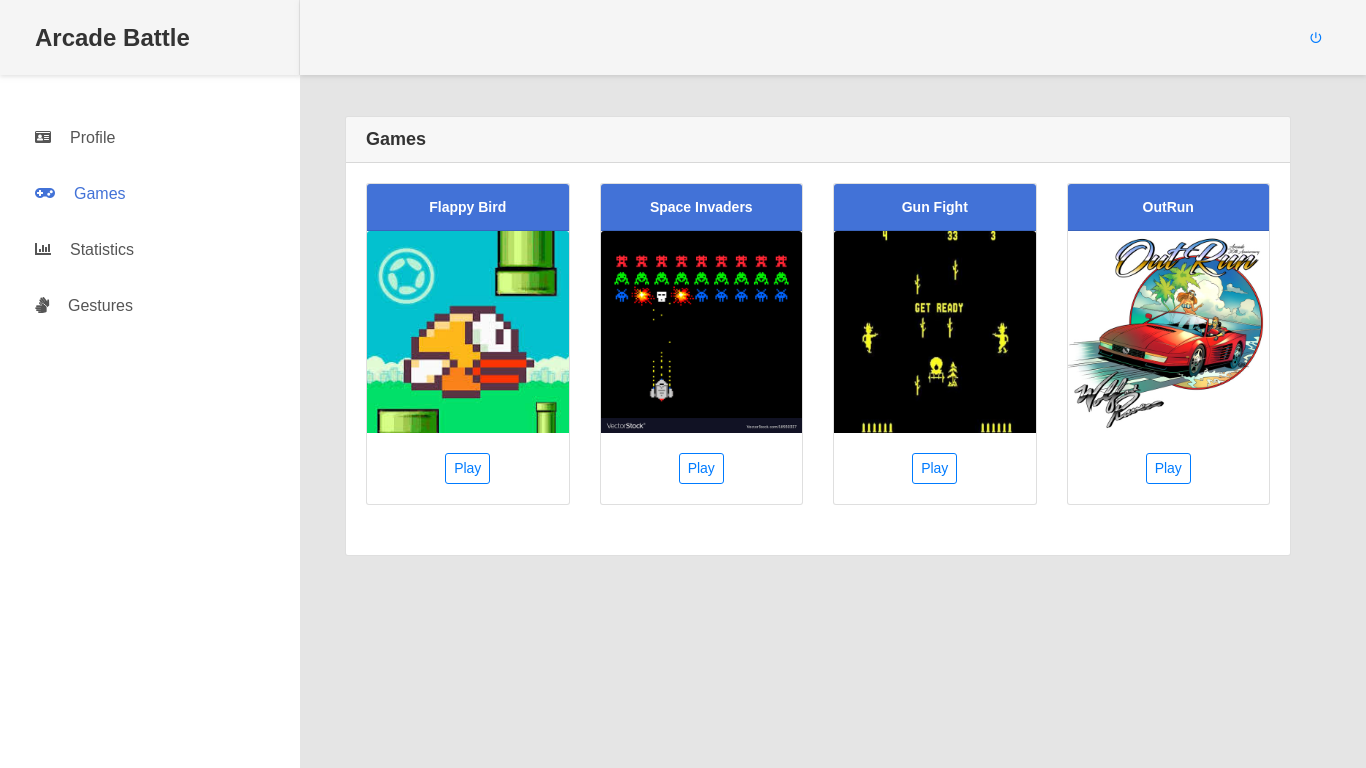
\includegraphics[scale=0.25]{./img/patient2.png}}
    \caption{Página dos jogos.}
    \label{fig:patient2}
\end{figure}

\begin{figure}[h!]
    \center
    \frame{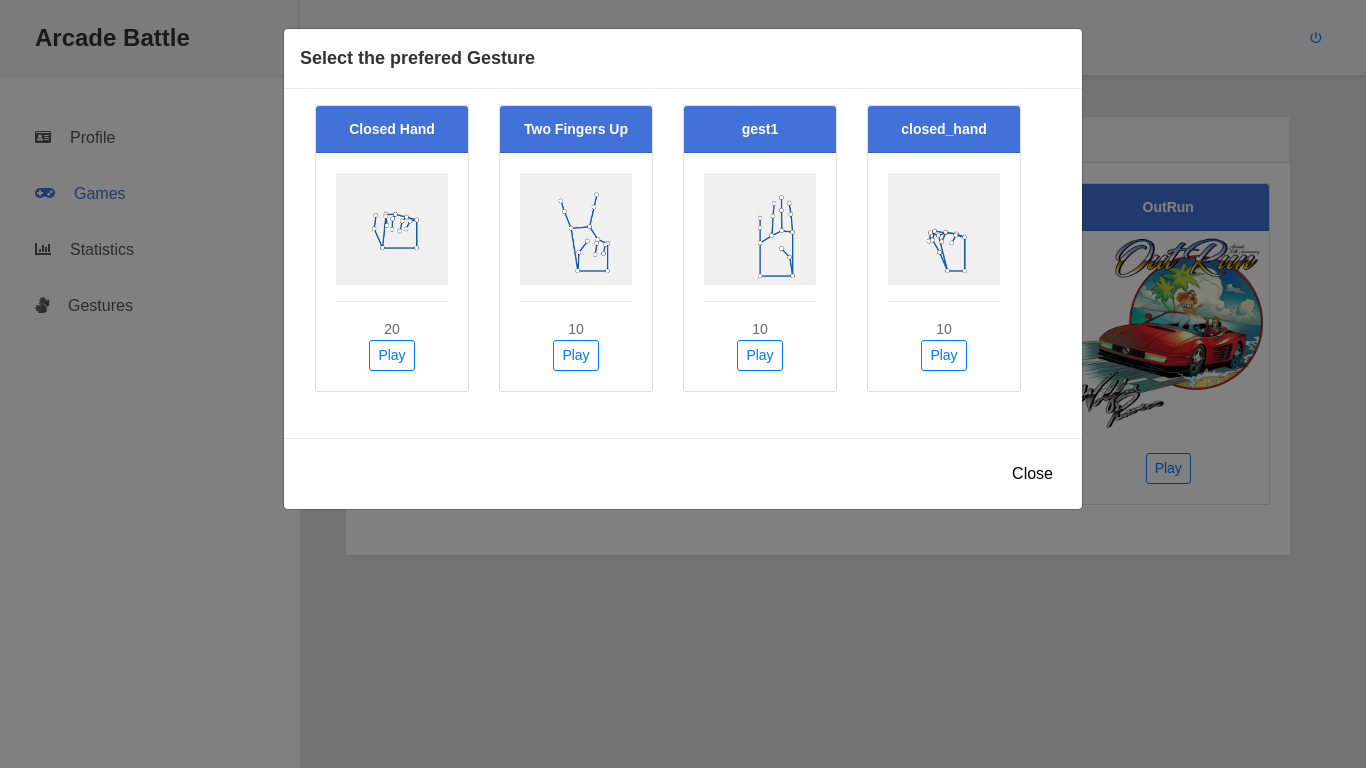
\includegraphics[scale=0.25]{./img/patient7.png}}
    \caption{Página para escolher gesto para jogar.}
    \label{fig:patient7}
\end{figure}

Após selecionar o gesto, o jogo começa e o paciente pode iniciar o tratamento.

\newpage

\subsubsection{Perfil}

No perfil o paciente encontra a informação sobre o seu médico, as notas que o mesmo deixou e também a possibilidade de alterar a password.

\begin{figure}[h!]
    \center
    \frame{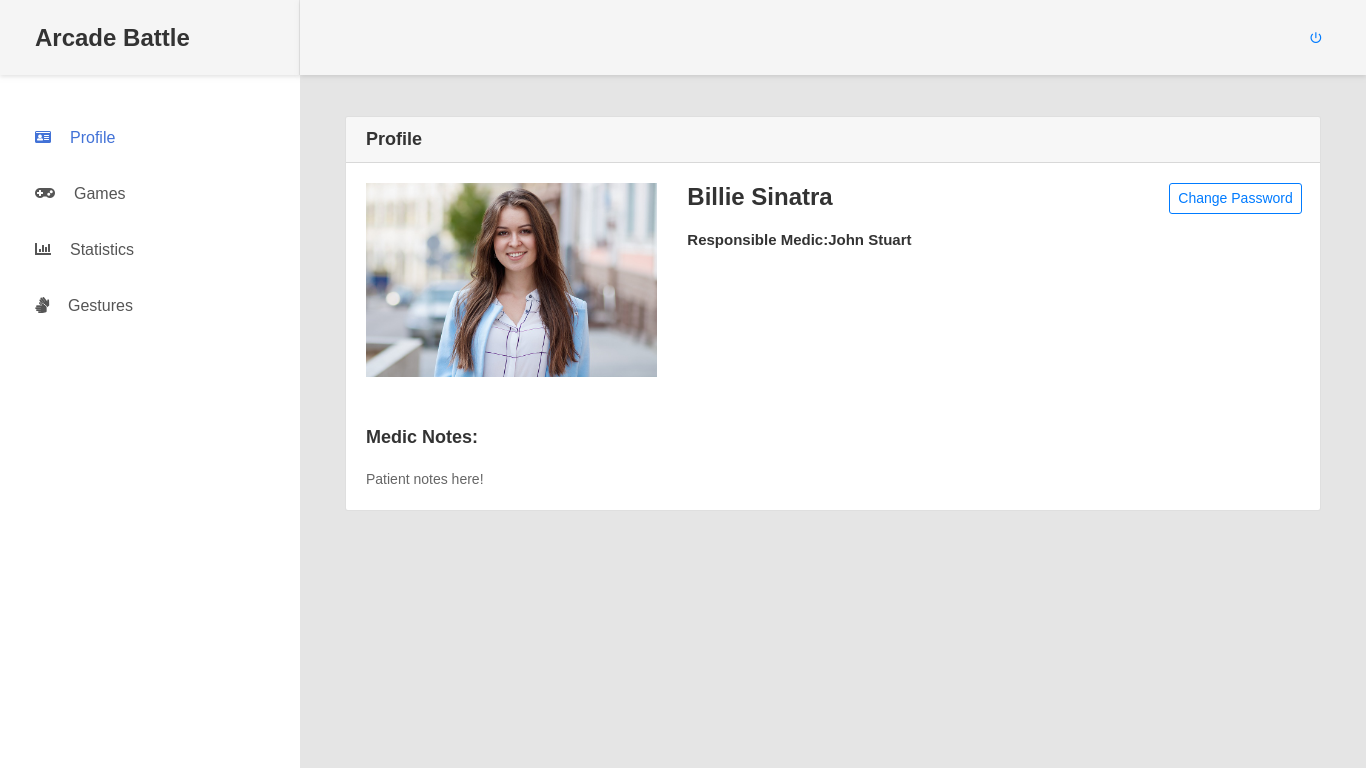
\includegraphics[scale=0.25]{./img/patient3.png}}
    \caption{Página do perfil do paciente.}
    \label{fig:patient3}
\end{figure}

\newpage

\subsubsection{Estatísticas}

Nesta aba o paciente pode observar graficamente a sua evolução. São apresentados gráficos referentes às pontuações obtidas[ figura abaixo]
em cada jogo e também referentes às repetições de cada gesto [duas figuras abaixo].

\begin{figure}[h!]
    \center
    \frame{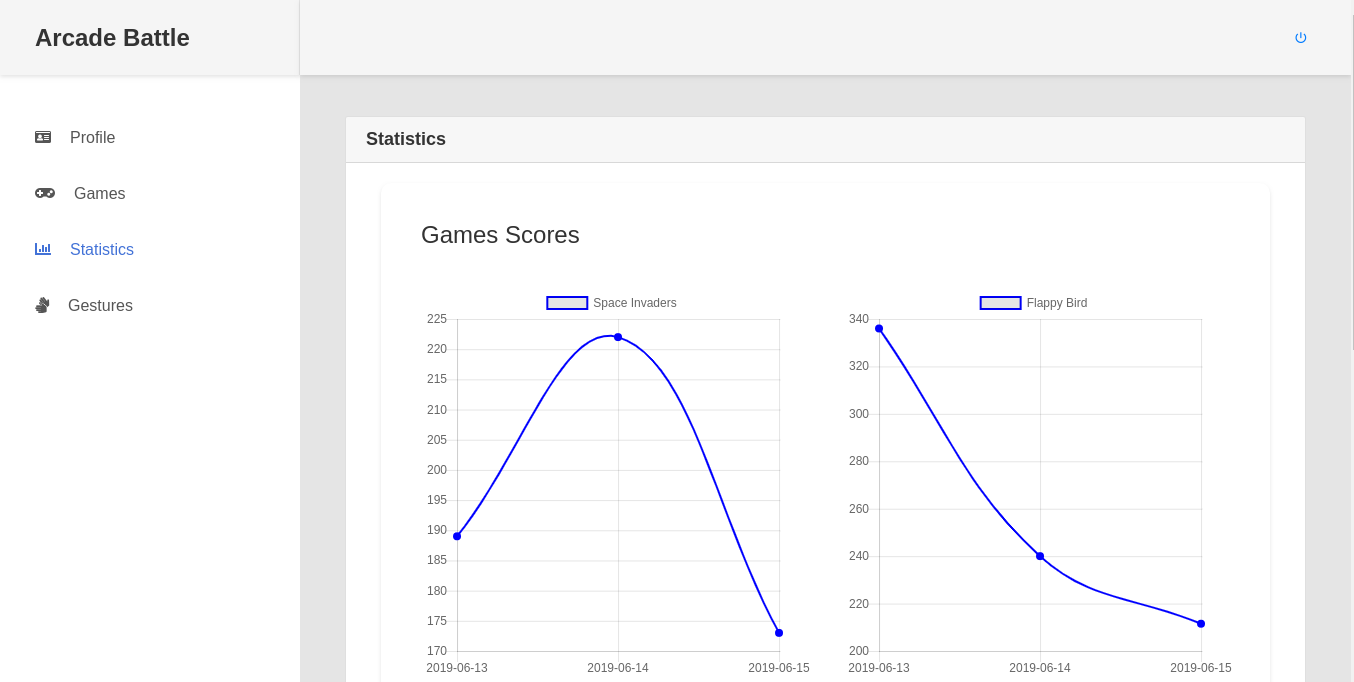
\includegraphics[scale=0.25]{./img/patient4.png}}
    \caption{Página das estatísticas.}
    \label{fig:patient4}
\end{figure}
\begin{figure}[h!]
    \center
    \frame{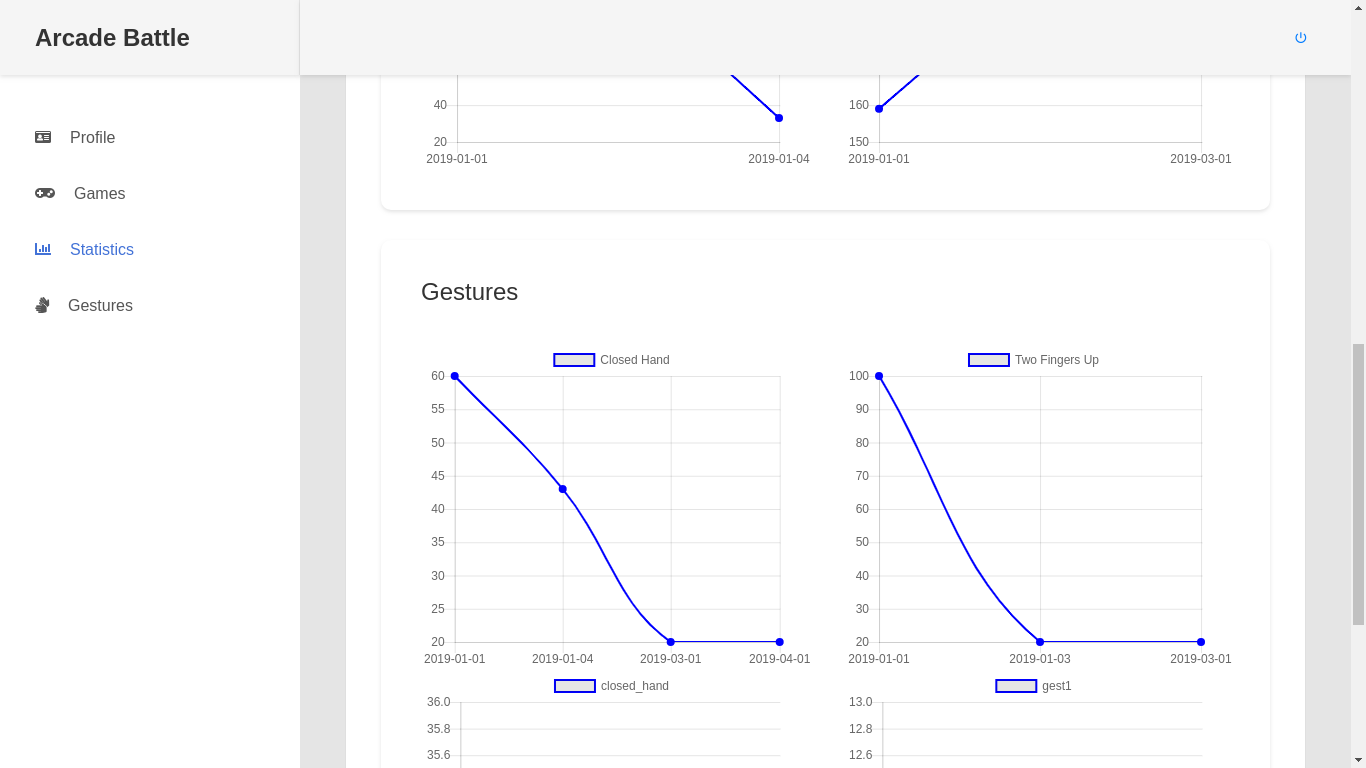
\includegraphics[scale=0.25]{./img/patient8.png}}
    \caption{Página das estatísticas.}
    \label{fig:patient8}
\end{figure}

Para a apresentação dos gráficos usamos a biblioteca chart.js, que permite criar gráficos segunda uma interface simples.

\newpage

\subsubsection{Gestos}

Nesta aba o paciente pode visualizar os gestos que pode realizar e as repetições que o médico definiu.

\begin{figure}[h!]
    \center
    \frame{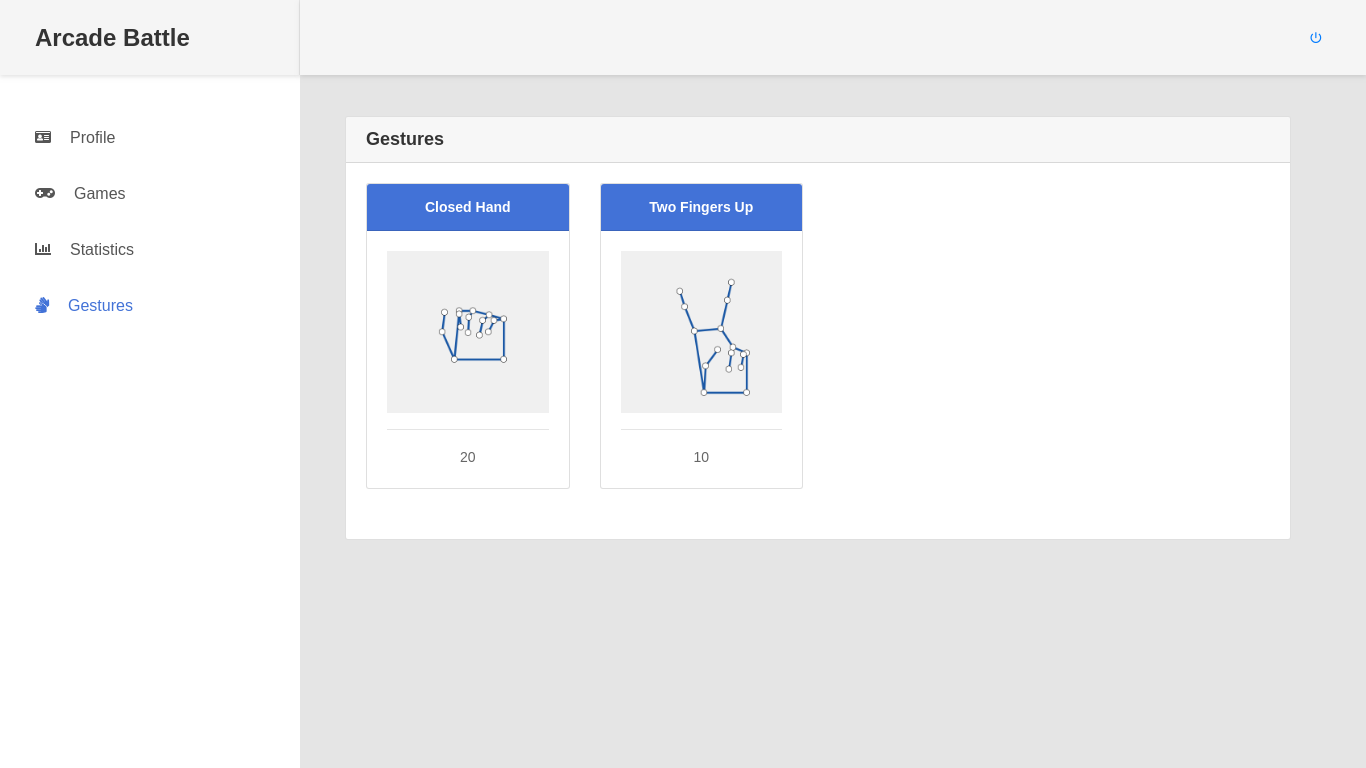
\includegraphics[scale=0.25]{./img/patient6.png}}
    \caption{Página dos gestos.}
    \label{fig:patient6}
\end{figure}

\subsection{Jogos}

Durante a recolha de requisitos, foi também necessário decidir se os jogos seriam construídos de raíz ou se utilizariamos soluções já implementadas.
De forma unânime, decidimos que o melhor seria implementarmos os jogos de raíz, pois, para além de aproveitarmos a oportunidade de aprender novas tecnologias/metodologias,
o mapeamento de um gesto para uma ação no jogo e a implementação da dificuldade dinâmica seriam menos complicadas de concretizar.

Posto isto, apesar de haver uma enorme variedade de tecnologias para implementar os jogos, era fundamental utilizar uma que, obrigatoriamente, cumprisse dois requisitos:

\begin{itemize}
	\item Ser escrita em JavaScript ou, no caso dos motores de jogo, ser possível exportar para um ficheiro JavaScript, uma vez que a aplicação do cliente
		  é um conjunto de páginas web transpostas no framework electron.
	\item Oferecer a capacidade de comunicar através de WebSockets como cliente.
\end{itemize}

Acabamos por reconhecer apenas duas opções viáveis: p5.js e Godot. Visto que nenhum elemento da equipa tinha experiência com um motor de jogo, optámos inicialmente por construir alguns jogos com p5.js, pois é apenas uma biblioteca do JavaScript, e, posteriormente, criar mais jogos, com Godot.

No final da implementação de todos os jogos, seria desejável, transpor para Godot todos os que estivessem escritos em p5.js.

\subsubsection{P5.JS}

P5.JS é uma biblioteca JavaScript que torna mais prática a tarefa de desenhar numa página Web, sendo também possível interagir com objetos HTML. É constituída por várias bibliotecas que funcionam como addons, e por isso, complementam as suas funcionalidades.

Para o nosso projeto, tal como foi acima referido, à medida que criámos os jogos, para além da biblioteca p5.js, também foi necessário fazer uso das seguintes bibliotecas:

\begin{itemize}
    \item p5.sound (implementação dos sons);
    \item p5.play (criação de Sprites no ambiente 2D);
    \item p5.dom (interação com elementos HTML);
    \item p5.collide2d (deteção de colisões).
\end{itemize}

Assim sendo, numa primeira fase, o foco principal foi criar cada jogo e garantir que funcionava corretamente, e por isso,
o emissor das ações a executar no jogo era o teclado do computador.

Seguidamente, entra a etapa onde o objetivo é garantir que a Leap Motion funcionava com o jogo. Nesta fase, já foi necessária a criação de WebSockets, e é aqui que aparece o nosso servidor, escrito em Node.js, para servir de ponte entre o jogo e a Leap Motion. Mais abaixo é explicado em detalhe toda a implementação das WebSockets, tanto ao nível do cliente, como ao nível do servidor.

Após a ligação e comunicação através de mensagens entre cliente-servidor estar a funcionar, começa a terceira fase, onde transpomos a aplicação do paciente e, consequentemente, os jogos para o framework Electron e garantimos que continua tudo a funcionar sem problemas. Esta foi, certamente, das fases mais complexas, pois aqui tivemos alguns problemas com as WebSockets, e necessitamos descobrir como era possível abrir uma nova janela e o jogo começar, imediatamente, no modo de ecrã inteiro.

Concluída esta etapa, surge a última fase, a da implementação da dificuldade dinâmica e do envio dos dados (número de gestos correta e incorretamente executados, pontuação no jogo, etc.) para a base de dados, quando o paciente perde ou sai do jogo. Assim sendo, recorremos, novamente, ao uso de WebSockets.
No final, terminámos com 4 jogos implementados com p5.js, sendo eles:

\begin{itemize}
	\item Flappy Bird.
	\item GunFight.
	\item Quizz.
	\item Space Invaders.
\end{itemize}

O GunFight não passou pela última fase, pois o propósito dele é ser um jogo para duas pessoas, ou seja, ter uma abordagem mais social, e o Quizz, apesar de estar desenvolvido,  precisa de ser reestruturado para os novos requisitos que entretanto foram adicionados/alterados.

\subsubsection{Godot}

Godot é um motor de jogos 2D e 3D, multiplataforma, lançado como software livre, e através do qual é possível criar jogos para computadores, telemóveis (mobile) e plataformas web. Este motor de jogos permite-nos programar os jogos nas linguagens C++, C# e GDScript (linguagem de scripting própria do Godot, muito parecida com Python).

Após os jogos escritos em p5.js estarem concretizados, decidimos experimentar esta tecnologia através da criação do jogo OutRun. Assim sendo, a diferença principal, comparativamente com a biblioteca p5.js, é o uso de cenários (scenes) para a construção do ambiente e objetos que constituem um jogo.

\begin{figure}[h!]
    \center
    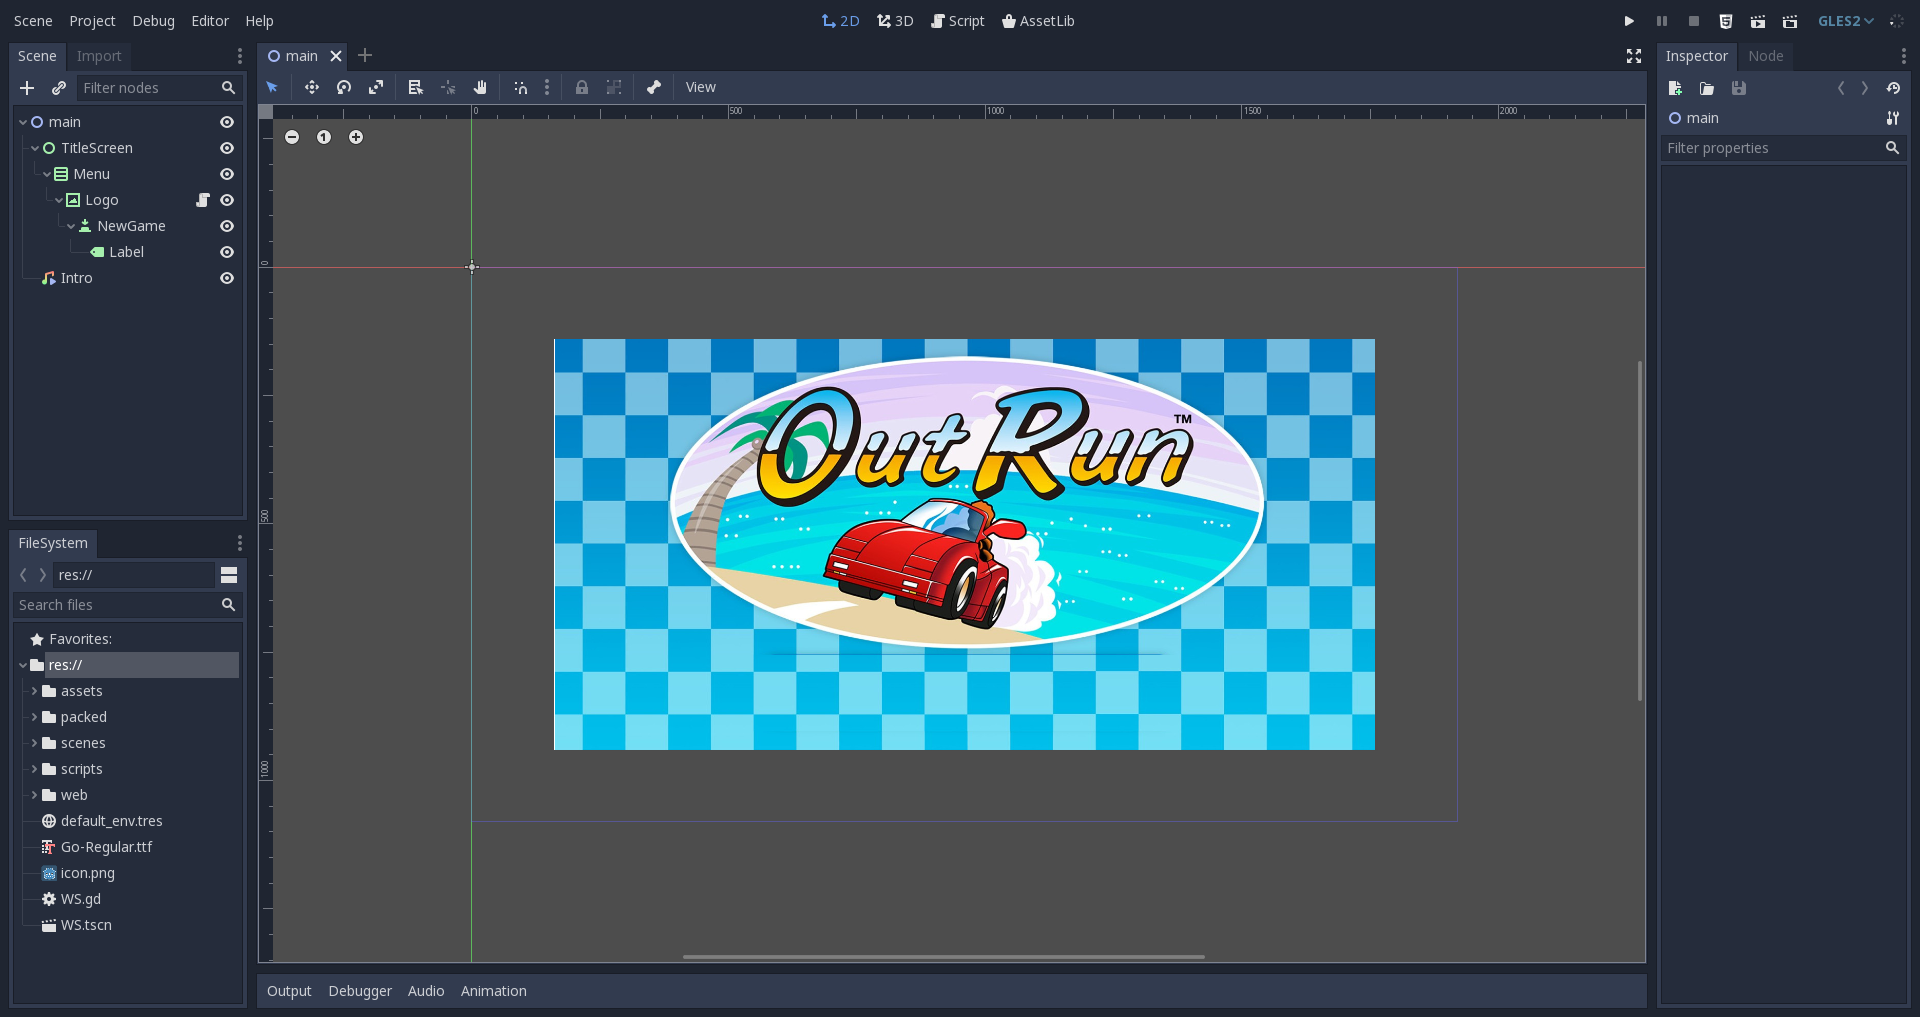
\includegraphics[scale=0.25]{./img/inicioGodot.png}
    \caption{Interface do motor de jogos Godot.}
    \label{fig:inicio_godot}
\end{figure}

Posteriormente à fase de exploração/aprendizagem, partimos para o desenvolvimento do jogo OutRun, onde descobrimos e aplicámos a linguagem de scripting própria do Godot,
o GDScript, de forma a trabalhar na lógica e efeitos do jogo.

A linguagem não foi difícil de aprender a usar, uma vez que é bastante semelhante com a linguagem python, porém, foi necessário aprender alguma da lógica implementada, como por exemplo, a existência de métodos por defeito para manipular o comportamento de um objeto. Uma característica interessante é a possibilidade de implementar a mesma função tanto na parte gráfica, com recurso aos cenários, como nos scripts, e tudo funciona em harmonia, mesmo que seja implementado das duas formas.

Assim que o jogo fica concluído e operacional, surge a parte mais difícil do desenvolvimento em Godot, a utilização de WebSockets como cliente, pois a informação existente sobre o tema é escassa, e a forma de implementação é proprietária. Contudo, a altura para usar esta tecnologia não podia ser melhor, pois a implementação oficial de WebSockets acontece na versão 3.1.

As motivações para usar WebSockets são exatamente as mesmas que nos jogos implementados com p5.js.
Solucionadas as dificuldades com WebSockets, apenas foi mandatório exportar o jogo para HTML/JavaScript.

E assim, com umas pequenas adições de código no ficheiro HTML, o jogo estava pronto a ser testado com a Leap Motion, a fim de garantir o ótimo funcionamento da aplicação.

\begin{figure}[h!]
    \center
    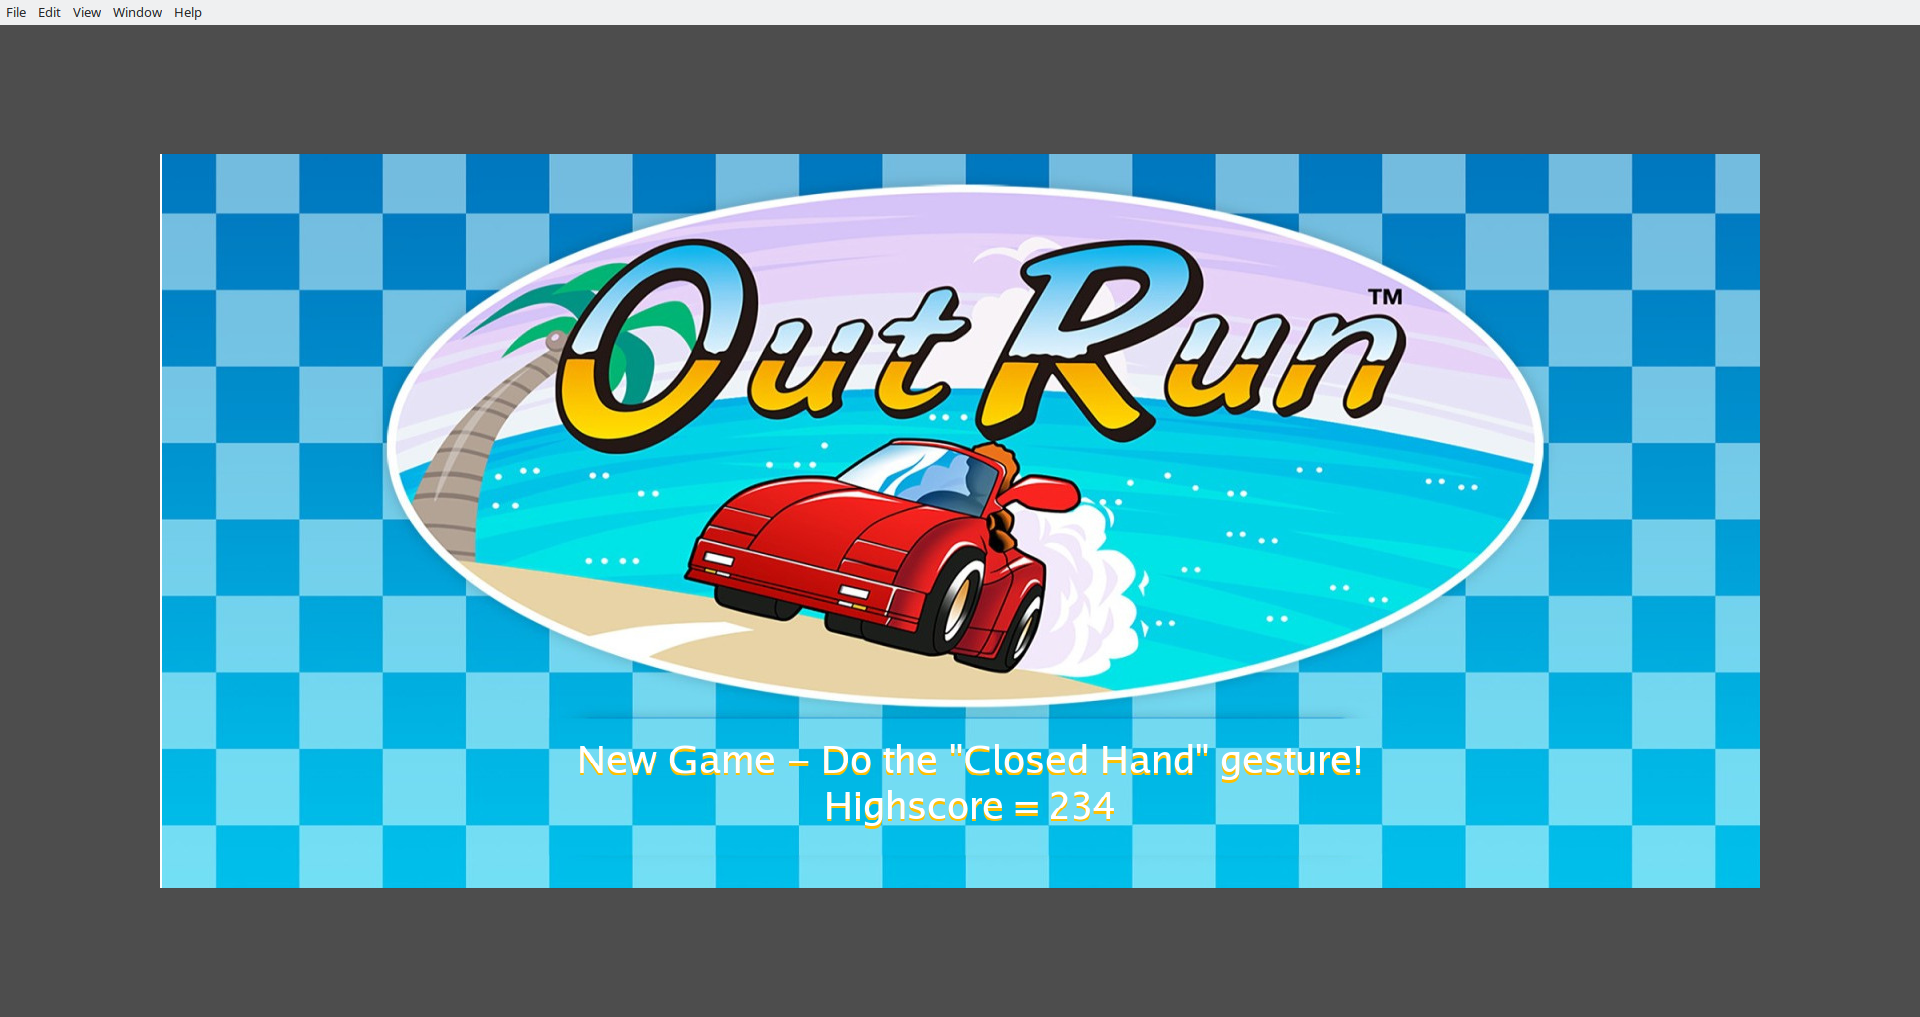
\includegraphics[scale=0.25]{./img/OutRun.png}
    \caption{Início do jogo outrun.}
    \label{fig:outrun}
\end{figure}

Terminados os jogos, e resta apenas dar um parecer sobre ambas as tecnologias, p5.js e Godot. Assim sendo, no resultado final, poucas são as diferenças que se podem encontrar ao nível visual, ou ao nível de desempenho, porém quando se trata do processo de desenvolvimento, o motor de jogos Godot é, significativamente, superior a p5.js.

Em Godot, apesar de ser uma ferramenta mais complicada de aprender do que p5.js, e por isso exigir mais tempo de prática, permite criar jogos em 2D ou 3D, sem requerer livrarias externas, de uma complexidade, significativamente, superior, e de uma forma mais limpa e apelativa à vista. Contudo esta comparação tende a ser injusta, visto que estamos a comparar um motor de jogos com uma simples biblioteca.

\subsubsection{Comunicação Entre Módulos}

Uma vez que optamos por construir um sistema totalmente desacoplado, eis que surge a implementação de WebSockets, para assim ser possível os módulos comunicarem entre si. Por esta razão, existem quatro WebSockets, todas a correr em localhost, por uma questão de latência:

\begin{itemize}
    \item game\_socket: funciona na porta 8081, e é onde acontece o transporte das mensagens, do tipo json, destinadas ao jogo, com o comando a executar no jogo;
    \item game\_stats\_socket: funciona na porta 8082, e é onde acontece o transporte das mensagens, do tipo json, destinadas ao jogo, com dados estatísticos sobre o desempenho do paciente naquele jogo. No final de cada partida, é por este socket que é enviada a mensagem, do tipo json, com os resultados;
    \item gesture\_recognition\_socket: funciona na porta 8080, e é onde acontece o transporte das mensagens, do tipo json, vindas da gesture\_recon.js, com o comando a executar no jogo;
    \item statistics\_socket: funciona na porta 8083, e é onde acontece o transporte das mensagens, do tipo json, vindas da base de dados, com dados estatísticos sobre o desempenho do paciente num determinado jogo.
\end{itemize}

Portanto, a origem das primeiras WebSockets implementadas, game\_socket e gesture\_recognition\_socket, acontece quando se começa a integrar a Leap Motion com os jogos. Visto que pretendíamos que fosse possível integrar qualquer forma de interagir com o computador (comandos de voz, teclado, gestos, etc.) para enviar comandos para o jogo, abstraímos essa questão com a implementação da classe main.js, responsável pelo envio das mensagens com os comandos a executar no jogo. Nesta fase, surgem as WebSockets game\_socket e~gesture\_recognition\_socket.

Com o desenvolvimento do projeto, surge a necessidade de enviar e receber dados provenientes da base de dados, para a implementação da dificuldade dinâmica e a visualização da pontuação máxima. Assim sendo, a nossa primeira abordagem foi implementar, em cada um dos jogos, as funções requeridas para que isso fosse possível.

Apesar de funcionar, ainda existe o problema de implementar as WebSockets e localStorage no jogo OutRun, pois não permite fazer alterações no código do jogo, depois deste ser exportado para HTML/JavaScript.

A partir daqui surge a classe statistics.js, com a finalidade de estabelecer a ligação entre o jogo e a base de dados, removendo o código duplicado e a exigência de usar o localStorage nas classes com os jogos. A comunicação é estabelecida entre os WebSockets game\_stats\_socket e statistics\_socket.

Porém, ainda faltava criar uma WebSocketClient do lado do jogo OutRun, que, inicialmente, pareceu ser complicada, mas que veio revelar-se simples, após entendermos a forma correta de funcionamento e estruturação das mensagens recebidas para poderem ser usadas como um dicionário.

\newpage

Após implementada a WebSocketClient no jogo OutRun pelos três cenários que o constituem, só faltava realizar os testes para garantir que todos os jogos estavam a funcionar como pretendido, que após estarem concluídos, deu resultado ao produto atual. Em relação aos tipos de mensagens json trocados entre os jogos, statistics.js e gesture\_recon.js, terminámos com 11 tipos diferentes:

\begin{itemize}
    \item "first\_message";
    \item "get\_statistics";
    \item "statistics";
    \item "statistics\_received";
    \item "gesture";
    \item "game\_started";
    \item "new\_difficulty";
    \item "difficulty";
    \item "game\_ended";
    \item "send\_score";
    \item "highscore".
\end{itemize}

% MÉTODOS USADOS PARA PARA IMPLEMENTAR O DESENHO DESCRITO ANTERIORMENTE.
% FORNECER INFORMAÇÃO PARA ALGUÉM REPLICAR O TRABALHO - COMO INSTALAR EM APÊNDIX.
% DIAGRAMAS E IMAGENS.

\section{Resultados}

Tivemos oportunidade de visitar o hospital de Aveiro, com o objetivo de testar o sistema como um todo e recolher o máximo feedback possível sobre a aplicação do paciente e do médico. As melhorias a realizar recaíram sobre a aplicação do médico, que já era expectável, visto que precisávamos desse feedback para compreender, por exemplo, quais os dados mais relevantes para um médico de forma a acompanhar o progresso dos seus pacientes.

Em termos da aplicação do paciente, as críticas incidiram sobre a deteção de gestos, por parte da Leap Motion, pois enquanto jogavam, os pacientes consideraram o equipamento lento e com falhas na detetação dos gestos. Dado que estes testes foram concretizados com gestos relativamente simples, no que toca a reconhecimento de gestos mais complexos, notoriamente, a situação agrava-se, pois existem gestos fundamentais para o tratamento que, simplesmente, não são exequíveis.

Este é um problema que, infelizmente, não conseguimos resolver, pois recai sobre as limitações do hardware da Leap Motion. Ao tentarmos encontrar uma alternativa para a Leap Motion, implementamos, com a tecnologia OpenCV, a deteção de gestos através da câmera frontal de um smartphone, porém a leitura era tão lenta (~10 fps) num smartphone topo de gama, que abandonámos imediatamente a ideia.

Por fim, apesar das limitações referidas acima, o projeto foi bem conseguido e superou expectativas, sendo que podemos classificar o feedback obtido como excelente, pois alguns dos pacientes que tiveram oportunidade de testar a aplicação do paciente, inserem-se nos utilizadores alvo da nossa plataforma, e os médicos, que testaram e ajudaram a melhorar a aplicação do médico, afirmaram que gostariam de continuar a trabalhar connosco, a fim de concretizar uma implementação real do sistema.

% ORGANIZAR RESULTADOS DO TRABALHO COM GRÁFICOS E TABELAS.
% ACRESCENTAR DISCUSSÃO SIGNIFICATIVA.
% DISCUTIR POSSÍVEIS FONTES DE ERRO E QUANTO PRECISOS OS RESULTADOS SÃO.
% Limitação do hardware ^^^.
% MOSTRAR O QUE NÃO RESOLVE/FUNCIONA.
% SUGERIR TRABALHO FUTURO.

\section{Conclusão}

O Arcade Battle é um sistema que tem como objetivo principal a motivação de pacientes que se encontrem a realizar reabilitação de artrite da mão. Tendo em conta que este tipo de reabilitação é um processo monótono para o paciente, o nosso sistema tem como objetivo utilizar os chamados ``Serious Games'' para que o paciente possa estar mais motivado a realizar o processo de reabilitação.

Estando agora o projeto concluído e olhando em retrospectiva, o projeto encontra-se numa fase onde se prevê uma possível comercialização do produto, fornecendo este a possibilidade
de adicionar novos gestos em menos de 1 minuto (incluindo tempo de treino da árvore de decisão) e precisões elevadas no reconhecimento de gestos.

Referir ainda que a arquitetura do projeto permite que todos os componentes sejam extremamente desacopláveis o que gera valor no sentido de facilmente mudar o processo de reabilitação da artrite na mão para algo como a terapia da fala, por exemplo, onde o jogo é agora controlado por comandos de voz.

Para trabalho futuro seria interessante estudar outras formas de input mais eficiente, tentando assim substituir as limitações provenientes do Leap Motion. Quanto ao reconhecimento de gestos, um estudo maior sobre este módulo poderia também ser uma vantagem trazendo a possibilidade de reconhecer gestos mais complexos.

\begin{thebibliography}{9}
\addcontentsline{toc}{section}{Referências}

\bibitem{rehability}
    Corona \textit{et al.},
    \textit{Serious Games for Wrist Rehabilitation in Juvenile Idiopathic Arthritis},
    2 Maio 2018.

\bibitem{poznan}
    Nowicki \textit{et al.},
    \textit{Gesture Recognition Library for Leap Motion Controller},
    Poznan University of Technology, 2014.

\bibitem{mit}
    Gillian \textit{et al.},
    \textit{The Gesture Recognition Toolkit}, in New England Machine Learning Day,
    2012.

\bibitem{handGestureReconWithLMC}
    Du \textit{et al.},
    \textit{Hand Gesture Recognition with Leap Motion},
    2017.

\bibitem{linshao}
    Lin Shao,
    \textit{Hand movement and gesture recognition using Leap Motion Controller},
    Stanford University, 2016.

\bibitem{survey}
    Moreira e Reis,
    \textit{Serious Games for Rehabilitation},
    2010.

\end{thebibliography}

\end{document}
